
% Default to the notebook output style

    


% Inherit from the specified cell style.




    
\documentclass[11pt]{article}

    
    
    \usepackage[T1]{fontenc}
    % Nicer default font (+ math font) than Computer Modern for most use cases
    \usepackage{mathpazo}

    % Basic figure setup, for now with no caption control since it's done
    % automatically by Pandoc (which extracts ![](path) syntax from Markdown).
    \usepackage{graphicx}
    % We will generate all images so they have a width \maxwidth. This means
    % that they will get their normal width if they fit onto the page, but
    % are scaled down if they would overflow the margins.
    \makeatletter
    \def\maxwidth{\ifdim\Gin@nat@width>\linewidth\linewidth
    \else\Gin@nat@width\fi}
    \makeatother
    \let\Oldincludegraphics\includegraphics
    % Set max figure width to be 80% of text width, for now hardcoded.
    \renewcommand{\includegraphics}[1]{\Oldincludegraphics[width=.8\maxwidth]{#1}}
    % Ensure that by default, figures have no caption (until we provide a
    % proper Figure object with a Caption API and a way to capture that
    % in the conversion process - todo).
    \usepackage{caption}
    \DeclareCaptionLabelFormat{nolabel}{}
    \captionsetup{labelformat=nolabel}

    \usepackage{adjustbox} % Used to constrain images to a maximum size 
    \usepackage{xcolor} % Allow colors to be defined
    \usepackage{enumerate} % Needed for markdown enumerations to work
    \usepackage{geometry} % Used to adjust the document margins
    \usepackage{amsmath} % Equations
    \usepackage{amssymb} % Equations
    \usepackage{textcomp} % defines textquotesingle
    % Hack from http://tex.stackexchange.com/a/47451/13684:
    \AtBeginDocument{%
        \def\PYZsq{\textquotesingle}% Upright quotes in Pygmentized code
    }
    \usepackage{upquote} % Upright quotes for verbatim code
    \usepackage{eurosym} % defines \euro
    \usepackage[mathletters]{ucs} % Extended unicode (utf-8) support
    \usepackage[utf8x]{inputenc} % Allow utf-8 characters in the tex document
    \usepackage{fancyvrb} % verbatim replacement that allows latex
    \usepackage{grffile} % extends the file name processing of package graphics 
                         % to support a larger range 
    % The hyperref package gives us a pdf with properly built
    % internal navigation ('pdf bookmarks' for the table of contents,
    % internal cross-reference links, web links for URLs, etc.)
    \usepackage{hyperref}
    \usepackage{longtable} % longtable support required by pandoc >1.10
    \usepackage{booktabs}  % table support for pandoc > 1.12.2
    \usepackage[inline]{enumitem} % IRkernel/repr support (it uses the enumerate* environment)
    \usepackage[normalem]{ulem} % ulem is needed to support strikethroughs (\sout)
                                % normalem makes italics be italics, not underlines
    

    
    
    % Colors for the hyperref package
    \definecolor{urlcolor}{rgb}{0,.145,.698}
    \definecolor{linkcolor}{rgb}{.71,0.21,0.01}
    \definecolor{citecolor}{rgb}{.12,.54,.11}

    % ANSI colors
    \definecolor{ansi-black}{HTML}{3E424D}
    \definecolor{ansi-black-intense}{HTML}{282C36}
    \definecolor{ansi-red}{HTML}{E75C58}
    \definecolor{ansi-red-intense}{HTML}{B22B31}
    \definecolor{ansi-green}{HTML}{00A250}
    \definecolor{ansi-green-intense}{HTML}{007427}
    \definecolor{ansi-yellow}{HTML}{DDB62B}
    \definecolor{ansi-yellow-intense}{HTML}{B27D12}
    \definecolor{ansi-blue}{HTML}{208FFB}
    \definecolor{ansi-blue-intense}{HTML}{0065CA}
    \definecolor{ansi-magenta}{HTML}{D160C4}
    \definecolor{ansi-magenta-intense}{HTML}{A03196}
    \definecolor{ansi-cyan}{HTML}{60C6C8}
    \definecolor{ansi-cyan-intense}{HTML}{258F8F}
    \definecolor{ansi-white}{HTML}{C5C1B4}
    \definecolor{ansi-white-intense}{HTML}{A1A6B2}

    % commands and environments needed by pandoc snippets
    % extracted from the output of `pandoc -s`
    \providecommand{\tightlist}{%
      \setlength{\itemsep}{0pt}\setlength{\parskip}{0pt}}
    \DefineVerbatimEnvironment{Highlighting}{Verbatim}{commandchars=\\\{\}}
    % Add ',fontsize=\small' for more characters per line
    \newenvironment{Shaded}{}{}
    \newcommand{\KeywordTok}[1]{\textcolor[rgb]{0.00,0.44,0.13}{\textbf{{#1}}}}
    \newcommand{\DataTypeTok}[1]{\textcolor[rgb]{0.56,0.13,0.00}{{#1}}}
    \newcommand{\DecValTok}[1]{\textcolor[rgb]{0.25,0.63,0.44}{{#1}}}
    \newcommand{\BaseNTok}[1]{\textcolor[rgb]{0.25,0.63,0.44}{{#1}}}
    \newcommand{\FloatTok}[1]{\textcolor[rgb]{0.25,0.63,0.44}{{#1}}}
    \newcommand{\CharTok}[1]{\textcolor[rgb]{0.25,0.44,0.63}{{#1}}}
    \newcommand{\StringTok}[1]{\textcolor[rgb]{0.25,0.44,0.63}{{#1}}}
    \newcommand{\CommentTok}[1]{\textcolor[rgb]{0.38,0.63,0.69}{\textit{{#1}}}}
    \newcommand{\OtherTok}[1]{\textcolor[rgb]{0.00,0.44,0.13}{{#1}}}
    \newcommand{\AlertTok}[1]{\textcolor[rgb]{1.00,0.00,0.00}{\textbf{{#1}}}}
    \newcommand{\FunctionTok}[1]{\textcolor[rgb]{0.02,0.16,0.49}{{#1}}}
    \newcommand{\RegionMarkerTok}[1]{{#1}}
    \newcommand{\ErrorTok}[1]{\textcolor[rgb]{1.00,0.00,0.00}{\textbf{{#1}}}}
    \newcommand{\NormalTok}[1]{{#1}}
    
    % Additional commands for more recent versions of Pandoc
    \newcommand{\ConstantTok}[1]{\textcolor[rgb]{0.53,0.00,0.00}{{#1}}}
    \newcommand{\SpecialCharTok}[1]{\textcolor[rgb]{0.25,0.44,0.63}{{#1}}}
    \newcommand{\VerbatimStringTok}[1]{\textcolor[rgb]{0.25,0.44,0.63}{{#1}}}
    \newcommand{\SpecialStringTok}[1]{\textcolor[rgb]{0.73,0.40,0.53}{{#1}}}
    \newcommand{\ImportTok}[1]{{#1}}
    \newcommand{\DocumentationTok}[1]{\textcolor[rgb]{0.73,0.13,0.13}{\textit{{#1}}}}
    \newcommand{\AnnotationTok}[1]{\textcolor[rgb]{0.38,0.63,0.69}{\textbf{\textit{{#1}}}}}
    \newcommand{\CommentVarTok}[1]{\textcolor[rgb]{0.38,0.63,0.69}{\textbf{\textit{{#1}}}}}
    \newcommand{\VariableTok}[1]{\textcolor[rgb]{0.10,0.09,0.49}{{#1}}}
    \newcommand{\ControlFlowTok}[1]{\textcolor[rgb]{0.00,0.44,0.13}{\textbf{{#1}}}}
    \newcommand{\OperatorTok}[1]{\textcolor[rgb]{0.40,0.40,0.40}{{#1}}}
    \newcommand{\BuiltInTok}[1]{{#1}}
    \newcommand{\ExtensionTok}[1]{{#1}}
    \newcommand{\PreprocessorTok}[1]{\textcolor[rgb]{0.74,0.48,0.00}{{#1}}}
    \newcommand{\AttributeTok}[1]{\textcolor[rgb]{0.49,0.56,0.16}{{#1}}}
    \newcommand{\InformationTok}[1]{\textcolor[rgb]{0.38,0.63,0.69}{\textbf{\textit{{#1}}}}}
    \newcommand{\WarningTok}[1]{\textcolor[rgb]{0.38,0.63,0.69}{\textbf{\textit{{#1}}}}}
    
    
    % Define a nice break command that doesn't care if a line doesn't already
    % exist.
    \def\br{\hspace*{\fill} \\* }
    % Math Jax compatability definitions
    \def\gt{>}
    \def\lt{<}
    % Document parameters
    \title{Wearable Devices using Dynamic Time Warping}
    
    
    

    % Pygments definitions
    
\makeatletter
\def\PY@reset{\let\PY@it=\relax \let\PY@bf=\relax%
    \let\PY@ul=\relax \let\PY@tc=\relax%
    \let\PY@bc=\relax \let\PY@ff=\relax}
\def\PY@tok#1{\csname PY@tok@#1\endcsname}
\def\PY@toks#1+{\ifx\relax#1\empty\else%
    \PY@tok{#1}\expandafter\PY@toks\fi}
\def\PY@do#1{\PY@bc{\PY@tc{\PY@ul{%
    \PY@it{\PY@bf{\PY@ff{#1}}}}}}}
\def\PY#1#2{\PY@reset\PY@toks#1+\relax+\PY@do{#2}}

\expandafter\def\csname PY@tok@w\endcsname{\def\PY@tc##1{\textcolor[rgb]{0.73,0.73,0.73}{##1}}}
\expandafter\def\csname PY@tok@c\endcsname{\let\PY@it=\textit\def\PY@tc##1{\textcolor[rgb]{0.25,0.50,0.50}{##1}}}
\expandafter\def\csname PY@tok@cp\endcsname{\def\PY@tc##1{\textcolor[rgb]{0.74,0.48,0.00}{##1}}}
\expandafter\def\csname PY@tok@k\endcsname{\let\PY@bf=\textbf\def\PY@tc##1{\textcolor[rgb]{0.00,0.50,0.00}{##1}}}
\expandafter\def\csname PY@tok@kp\endcsname{\def\PY@tc##1{\textcolor[rgb]{0.00,0.50,0.00}{##1}}}
\expandafter\def\csname PY@tok@kt\endcsname{\def\PY@tc##1{\textcolor[rgb]{0.69,0.00,0.25}{##1}}}
\expandafter\def\csname PY@tok@o\endcsname{\def\PY@tc##1{\textcolor[rgb]{0.40,0.40,0.40}{##1}}}
\expandafter\def\csname PY@tok@ow\endcsname{\let\PY@bf=\textbf\def\PY@tc##1{\textcolor[rgb]{0.67,0.13,1.00}{##1}}}
\expandafter\def\csname PY@tok@nb\endcsname{\def\PY@tc##1{\textcolor[rgb]{0.00,0.50,0.00}{##1}}}
\expandafter\def\csname PY@tok@nf\endcsname{\def\PY@tc##1{\textcolor[rgb]{0.00,0.00,1.00}{##1}}}
\expandafter\def\csname PY@tok@nc\endcsname{\let\PY@bf=\textbf\def\PY@tc##1{\textcolor[rgb]{0.00,0.00,1.00}{##1}}}
\expandafter\def\csname PY@tok@nn\endcsname{\let\PY@bf=\textbf\def\PY@tc##1{\textcolor[rgb]{0.00,0.00,1.00}{##1}}}
\expandafter\def\csname PY@tok@ne\endcsname{\let\PY@bf=\textbf\def\PY@tc##1{\textcolor[rgb]{0.82,0.25,0.23}{##1}}}
\expandafter\def\csname PY@tok@nv\endcsname{\def\PY@tc##1{\textcolor[rgb]{0.10,0.09,0.49}{##1}}}
\expandafter\def\csname PY@tok@no\endcsname{\def\PY@tc##1{\textcolor[rgb]{0.53,0.00,0.00}{##1}}}
\expandafter\def\csname PY@tok@nl\endcsname{\def\PY@tc##1{\textcolor[rgb]{0.63,0.63,0.00}{##1}}}
\expandafter\def\csname PY@tok@ni\endcsname{\let\PY@bf=\textbf\def\PY@tc##1{\textcolor[rgb]{0.60,0.60,0.60}{##1}}}
\expandafter\def\csname PY@tok@na\endcsname{\def\PY@tc##1{\textcolor[rgb]{0.49,0.56,0.16}{##1}}}
\expandafter\def\csname PY@tok@nt\endcsname{\let\PY@bf=\textbf\def\PY@tc##1{\textcolor[rgb]{0.00,0.50,0.00}{##1}}}
\expandafter\def\csname PY@tok@nd\endcsname{\def\PY@tc##1{\textcolor[rgb]{0.67,0.13,1.00}{##1}}}
\expandafter\def\csname PY@tok@s\endcsname{\def\PY@tc##1{\textcolor[rgb]{0.73,0.13,0.13}{##1}}}
\expandafter\def\csname PY@tok@sd\endcsname{\let\PY@it=\textit\def\PY@tc##1{\textcolor[rgb]{0.73,0.13,0.13}{##1}}}
\expandafter\def\csname PY@tok@si\endcsname{\let\PY@bf=\textbf\def\PY@tc##1{\textcolor[rgb]{0.73,0.40,0.53}{##1}}}
\expandafter\def\csname PY@tok@se\endcsname{\let\PY@bf=\textbf\def\PY@tc##1{\textcolor[rgb]{0.73,0.40,0.13}{##1}}}
\expandafter\def\csname PY@tok@sr\endcsname{\def\PY@tc##1{\textcolor[rgb]{0.73,0.40,0.53}{##1}}}
\expandafter\def\csname PY@tok@ss\endcsname{\def\PY@tc##1{\textcolor[rgb]{0.10,0.09,0.49}{##1}}}
\expandafter\def\csname PY@tok@sx\endcsname{\def\PY@tc##1{\textcolor[rgb]{0.00,0.50,0.00}{##1}}}
\expandafter\def\csname PY@tok@m\endcsname{\def\PY@tc##1{\textcolor[rgb]{0.40,0.40,0.40}{##1}}}
\expandafter\def\csname PY@tok@gh\endcsname{\let\PY@bf=\textbf\def\PY@tc##1{\textcolor[rgb]{0.00,0.00,0.50}{##1}}}
\expandafter\def\csname PY@tok@gu\endcsname{\let\PY@bf=\textbf\def\PY@tc##1{\textcolor[rgb]{0.50,0.00,0.50}{##1}}}
\expandafter\def\csname PY@tok@gd\endcsname{\def\PY@tc##1{\textcolor[rgb]{0.63,0.00,0.00}{##1}}}
\expandafter\def\csname PY@tok@gi\endcsname{\def\PY@tc##1{\textcolor[rgb]{0.00,0.63,0.00}{##1}}}
\expandafter\def\csname PY@tok@gr\endcsname{\def\PY@tc##1{\textcolor[rgb]{1.00,0.00,0.00}{##1}}}
\expandafter\def\csname PY@tok@ge\endcsname{\let\PY@it=\textit}
\expandafter\def\csname PY@tok@gs\endcsname{\let\PY@bf=\textbf}
\expandafter\def\csname PY@tok@gp\endcsname{\let\PY@bf=\textbf\def\PY@tc##1{\textcolor[rgb]{0.00,0.00,0.50}{##1}}}
\expandafter\def\csname PY@tok@go\endcsname{\def\PY@tc##1{\textcolor[rgb]{0.53,0.53,0.53}{##1}}}
\expandafter\def\csname PY@tok@gt\endcsname{\def\PY@tc##1{\textcolor[rgb]{0.00,0.27,0.87}{##1}}}
\expandafter\def\csname PY@tok@err\endcsname{\def\PY@bc##1{\setlength{\fboxsep}{0pt}\fcolorbox[rgb]{1.00,0.00,0.00}{1,1,1}{\strut ##1}}}
\expandafter\def\csname PY@tok@kc\endcsname{\let\PY@bf=\textbf\def\PY@tc##1{\textcolor[rgb]{0.00,0.50,0.00}{##1}}}
\expandafter\def\csname PY@tok@kd\endcsname{\let\PY@bf=\textbf\def\PY@tc##1{\textcolor[rgb]{0.00,0.50,0.00}{##1}}}
\expandafter\def\csname PY@tok@kn\endcsname{\let\PY@bf=\textbf\def\PY@tc##1{\textcolor[rgb]{0.00,0.50,0.00}{##1}}}
\expandafter\def\csname PY@tok@kr\endcsname{\let\PY@bf=\textbf\def\PY@tc##1{\textcolor[rgb]{0.00,0.50,0.00}{##1}}}
\expandafter\def\csname PY@tok@bp\endcsname{\def\PY@tc##1{\textcolor[rgb]{0.00,0.50,0.00}{##1}}}
\expandafter\def\csname PY@tok@fm\endcsname{\def\PY@tc##1{\textcolor[rgb]{0.00,0.00,1.00}{##1}}}
\expandafter\def\csname PY@tok@vc\endcsname{\def\PY@tc##1{\textcolor[rgb]{0.10,0.09,0.49}{##1}}}
\expandafter\def\csname PY@tok@vg\endcsname{\def\PY@tc##1{\textcolor[rgb]{0.10,0.09,0.49}{##1}}}
\expandafter\def\csname PY@tok@vi\endcsname{\def\PY@tc##1{\textcolor[rgb]{0.10,0.09,0.49}{##1}}}
\expandafter\def\csname PY@tok@vm\endcsname{\def\PY@tc##1{\textcolor[rgb]{0.10,0.09,0.49}{##1}}}
\expandafter\def\csname PY@tok@sa\endcsname{\def\PY@tc##1{\textcolor[rgb]{0.73,0.13,0.13}{##1}}}
\expandafter\def\csname PY@tok@sb\endcsname{\def\PY@tc##1{\textcolor[rgb]{0.73,0.13,0.13}{##1}}}
\expandafter\def\csname PY@tok@sc\endcsname{\def\PY@tc##1{\textcolor[rgb]{0.73,0.13,0.13}{##1}}}
\expandafter\def\csname PY@tok@dl\endcsname{\def\PY@tc##1{\textcolor[rgb]{0.73,0.13,0.13}{##1}}}
\expandafter\def\csname PY@tok@s2\endcsname{\def\PY@tc##1{\textcolor[rgb]{0.73,0.13,0.13}{##1}}}
\expandafter\def\csname PY@tok@sh\endcsname{\def\PY@tc##1{\textcolor[rgb]{0.73,0.13,0.13}{##1}}}
\expandafter\def\csname PY@tok@s1\endcsname{\def\PY@tc##1{\textcolor[rgb]{0.73,0.13,0.13}{##1}}}
\expandafter\def\csname PY@tok@mb\endcsname{\def\PY@tc##1{\textcolor[rgb]{0.40,0.40,0.40}{##1}}}
\expandafter\def\csname PY@tok@mf\endcsname{\def\PY@tc##1{\textcolor[rgb]{0.40,0.40,0.40}{##1}}}
\expandafter\def\csname PY@tok@mh\endcsname{\def\PY@tc##1{\textcolor[rgb]{0.40,0.40,0.40}{##1}}}
\expandafter\def\csname PY@tok@mi\endcsname{\def\PY@tc##1{\textcolor[rgb]{0.40,0.40,0.40}{##1}}}
\expandafter\def\csname PY@tok@il\endcsname{\def\PY@tc##1{\textcolor[rgb]{0.40,0.40,0.40}{##1}}}
\expandafter\def\csname PY@tok@mo\endcsname{\def\PY@tc##1{\textcolor[rgb]{0.40,0.40,0.40}{##1}}}
\expandafter\def\csname PY@tok@ch\endcsname{\let\PY@it=\textit\def\PY@tc##1{\textcolor[rgb]{0.25,0.50,0.50}{##1}}}
\expandafter\def\csname PY@tok@cm\endcsname{\let\PY@it=\textit\def\PY@tc##1{\textcolor[rgb]{0.25,0.50,0.50}{##1}}}
\expandafter\def\csname PY@tok@cpf\endcsname{\let\PY@it=\textit\def\PY@tc##1{\textcolor[rgb]{0.25,0.50,0.50}{##1}}}
\expandafter\def\csname PY@tok@c1\endcsname{\let\PY@it=\textit\def\PY@tc##1{\textcolor[rgb]{0.25,0.50,0.50}{##1}}}
\expandafter\def\csname PY@tok@cs\endcsname{\let\PY@it=\textit\def\PY@tc##1{\textcolor[rgb]{0.25,0.50,0.50}{##1}}}

\def\PYZbs{\char`\\}
\def\PYZus{\char`\_}
\def\PYZob{\char`\{}
\def\PYZcb{\char`\}}
\def\PYZca{\char`\^}
\def\PYZam{\char`\&}
\def\PYZlt{\char`\<}
\def\PYZgt{\char`\>}
\def\PYZsh{\char`\#}
\def\PYZpc{\char`\%}
\def\PYZdl{\char`\$}
\def\PYZhy{\char`\-}
\def\PYZsq{\char`\'}
\def\PYZdq{\char`\"}
\def\PYZti{\char`\~}
% for compatibility with earlier versions
\def\PYZat{@}
\def\PYZlb{[}
\def\PYZrb{]}
\makeatother


    % Exact colors from NB
    \definecolor{incolor}{rgb}{0.0, 0.0, 0.5}
    \definecolor{outcolor}{rgb}{0.545, 0.0, 0.0}



    
    % Prevent overflowing lines due to hard-to-break entities
    \sloppy 
    % Setup hyperref package
    \hypersetup{
      breaklinks=true,  % so long urls are correctly broken across lines
      colorlinks=true,
      urlcolor=urlcolor,
      linkcolor=linkcolor,
      citecolor=citecolor,
      }
    % Slightly bigger margins than the latex defaults
    
    \geometry{verbose,tmargin=1in,bmargin=1in,lmargin=1in,rmargin=1in}
    
    

    \begin{document}
    
    
    \maketitle
    
    

    
    \section{COMP7404 Computational intelligence and machine
learning}\label{comp7404-computational-intelligence-and-machine-learning}

\section{Group Project - Peer Teaching -
Demo}\label{group-project---peer-teaching---demo}

    \section{Detailed Instructions - Preparations need to be done before
running
demo}\label{detailed-instructions---preparations-need-to-be-done-before-running-demo}

\paragraph{1. download GroupProject\_GroupN.zip from GitHub and unzip
it}\label{download-groupproject_groupn.zip-from-github-and-unzip-it}

\paragraph{2. go to the link below and download
MHEALTHDATASET.zip}\label{go-to-the-link-below-and-download-mhealthdataset.zip}

\paragraph{http://archive.ics.uci.edu/ml/machine-learning-databases/00319/}\label{httparchive.ics.uci.edumlmachine-learning-databases00319}

\paragraph{3. unzip MHEALTHDATASET.zip, then copy all 10 data files
(mHealth\_subjectX.log where X from 1 to 10) to the folder
"GroupProject\_GroupN"}\label{unzip-mhealthdataset.zip-then-copy-all-10-data-files-mhealth_subjectx.log-where-x-from-1-to-10-to-the-folder-groupproject_groupn}

\paragraph{4. make sure packages including numpy, scipy, fastdtw,
collections, plyfile, mpl\_toolkits.mplot3d, matplotlib and sklearn are
installed}\label{make-sure-packages-including-numpy-scipy-fastdtw-collections-plyfile-mpl_toolkits.mplot3d-matplotlib-and-sklearn-are-installed}

\paragraph{5. Python 3.6 is used}\label{python-3.6-is-used}

\paragraph{6. go to GroupProject\_GroupN folder and open jupyter
notebook named "Wearable Devices using Dynamic Time Warping.ipynb" to
run the
demo}\label{go-to-groupproject_groupn-folder-and-open-jupyter-notebook-named-wearable-devices-using-dynamic-time-warping.ipynb-to-run-the-demo}

    \section{Classes have been designed to manage datasets and algorithm
logic}\label{classes-have-been-designed-to-manage-datasets-and-algorithm-logic}

\subsection{superclass: dataset}\label{superclass-dataset}

\subsubsection{subclass:trainset}\label{subclasstrainset}

\subsubsection{subclass:testset}\label{subclasstestset}

\subsubsection{subclass:masterset}\label{subclassmasterset}

\subsection{superclass: Experiment}\label{superclass-experiment}

\subsubsection{subclass:DTWExperiment}\label{subclassdtwexperiment}

    \begin{Verbatim}[commandchars=\\\{\}]
{\color{incolor}In [{\color{incolor}1}]:} \PY{k+kn}{import} \PY{n+nn}{pandas} \PY{k}{as} \PY{n+nn}{pd}
        \PY{k+kn}{import} \PY{n+nn}{math}
        
        \PY{k}{class} \PY{n+nc}{dataset}\PY{p}{(}\PY{n+nb}{object}\PY{p}{)}\PY{p}{:}
            \PY{k}{def} \PY{n+nf}{\PYZus{}\PYZus{}init\PYZus{}\PYZus{}}\PY{p}{(}\PY{n+nb+bp}{self}\PY{p}{,} \PY{n}{data}\PY{p}{)}\PY{p}{:}
                \PY{n+nb+bp}{self}\PY{o}{.}\PY{n}{\PYZus{}data} \PY{o}{=} \PY{n}{data}
            
            \PY{k}{def} \PY{n+nf}{get\PYZus{}data}\PY{p}{(}\PY{n+nb+bp}{self}\PY{p}{)}\PY{p}{:}
                \PY{k}{return} \PY{n+nb+bp}{self}\PY{o}{.}\PY{n}{\PYZus{}data}
            
            \PY{k}{def} \PY{n+nf}{get\PYZus{}data\PYZus{}by\PYZus{}rows}\PY{p}{(}\PY{n+nb+bp}{self}\PY{p}{,} \PY{n}{no\PYZus{}of\PYZus{}rows}\PY{p}{)}\PY{p}{:}
                \PY{k}{return} \PY{n+nb+bp}{self}\PY{o}{.}\PY{n}{\PYZus{}data}\PY{p}{[}\PY{l+m+mi}{0}\PY{p}{:}\PY{n}{no\PYZus{}of\PYZus{}rows}\PY{p}{]}
            
            
            \PY{k}{def} \PY{n+nf}{data\PYZus{}cleaning}\PY{p}{(}\PY{n+nb+bp}{self}\PY{p}{)}\PY{p}{:}
                
        \PY{c+c1}{\PYZsh{}         print(\PYZsq{}before dropping na\PYZsq{}, self.\PYZus{}data.shape)}
        \PY{c+c1}{\PYZsh{}         self.\PYZus{}data.dropna(axis = 0, how=\PYZsq{}any\PYZsq{}, inplace = True)}
        \PY{c+c1}{\PYZsh{}         print(\PYZsq{}after dropping na\PYZsq{}, self.\PYZus{}data.shape)}
                
                \PY{n+nb}{print}\PY{p}{(}\PY{l+s+s1}{\PYZsq{}}\PY{l+s+s1}{before cleaning}\PY{l+s+s1}{\PYZsq{}}\PY{p}{,} \PY{n+nb+bp}{self}\PY{o}{.}\PY{n}{\PYZus{}data}\PY{o}{.}\PY{n}{Label}\PY{o}{.}\PY{n}{unique}\PY{p}{(}\PY{p}{)}\PY{p}{)}
                \PY{n+nb+bp}{self}\PY{o}{.}\PY{n}{\PYZus{}data} \PY{o}{=} \PY{n+nb+bp}{self}\PY{o}{.}\PY{n}{\PYZus{}data}\PY{p}{[}\PY{n+nb+bp}{self}\PY{o}{.}\PY{n}{\PYZus{}data}\PY{p}{[}\PY{l+s+s1}{\PYZsq{}}\PY{l+s+s1}{Label}\PY{l+s+s1}{\PYZsq{}}\PY{p}{]} \PY{o}{!=} \PY{l+m+mi}{0}\PY{p}{]}
                \PY{n+nb}{print}\PY{p}{(}\PY{l+s+s1}{\PYZsq{}}\PY{l+s+s1}{after cleaning}\PY{l+s+s1}{\PYZsq{}}\PY{p}{,} \PY{n+nb+bp}{self}\PY{o}{.}\PY{n}{\PYZus{}data}\PY{o}{.}\PY{n}{Label}\PY{o}{.}\PY{n}{unique}\PY{p}{(}\PY{p}{)}\PY{p}{)}
        
        
                
            \PY{k}{def} \PY{n+nf}{data\PYZus{}selected\PYZus{}features}\PY{p}{(}\PY{n+nb+bp}{self}\PY{p}{,} \PY{n}{selectedFeatures}\PY{p}{)}\PY{p}{:}
                \PY{n+nb}{print}\PY{p}{(}\PY{l+s+s1}{\PYZsq{}}\PY{l+s+s1}{before features selected}\PY{l+s+s1}{\PYZsq{}}\PY{p}{,} \PY{n+nb+bp}{self}\PY{o}{.}\PY{n}{\PYZus{}data}\PY{o}{.}\PY{n}{columns}\PY{o}{.}\PY{n}{unique}\PY{p}{(}\PY{p}{)}\PY{p}{)}
                \PY{n+nb+bp}{self}\PY{o}{.}\PY{n}{\PYZus{}data} \PY{o}{=} \PY{n+nb+bp}{self}\PY{o}{.}\PY{n}{\PYZus{}data}\PY{p}{[}\PY{n}{selectedFeatures}\PY{p}{]}
                \PY{n+nb}{print}\PY{p}{(}\PY{l+s+s1}{\PYZsq{}}\PY{l+s+s1}{after features selected}\PY{l+s+s1}{\PYZsq{}}\PY{p}{,} \PY{n+nb+bp}{self}\PY{o}{.}\PY{n}{\PYZus{}data}\PY{o}{.}\PY{n}{columns}\PY{o}{.}\PY{n}{unique}\PY{p}{(}\PY{p}{)}\PY{p}{)}
                
            
            \PY{k}{def} \PY{n+nf}{data\PYZus{}selected\PYZus{}labels}\PY{p}{(}\PY{n+nb+bp}{self}\PY{p}{,} \PY{n}{selectedLabels}\PY{p}{)}\PY{p}{:}
                \PY{n+nb}{print}\PY{p}{(}\PY{l+s+s1}{\PYZsq{}}\PY{l+s+s1}{before labels selected}\PY{l+s+s1}{\PYZsq{}}\PY{p}{,} \PY{n+nb+bp}{self}\PY{o}{.}\PY{n}{\PYZus{}data}\PY{o}{.}\PY{n}{Label}\PY{o}{.}\PY{n}{unique}\PY{p}{(}\PY{p}{)}\PY{p}{)}
                \PY{n+nb+bp}{self}\PY{o}{.}\PY{n}{\PYZus{}data} \PY{o}{=} \PY{n+nb+bp}{self}\PY{o}{.}\PY{n}{\PYZus{}data}\PY{p}{[}\PY{n+nb+bp}{self}\PY{o}{.}\PY{n}{\PYZus{}data}\PY{p}{[}\PY{l+s+s1}{\PYZsq{}}\PY{l+s+s1}{Label}\PY{l+s+s1}{\PYZsq{}}\PY{p}{]}\PY{o}{.}\PY{n}{isin}\PY{p}{(}\PY{n}{selectedLabels}\PY{p}{)}\PY{p}{]}
                \PY{n+nb}{print}\PY{p}{(}\PY{l+s+s1}{\PYZsq{}}\PY{l+s+s1}{after labels selected}\PY{l+s+s1}{\PYZsq{}}\PY{p}{,} \PY{n+nb+bp}{self}\PY{o}{.}\PY{n}{\PYZus{}data}\PY{o}{.}\PY{n}{Label}\PY{o}{.}\PY{n}{unique}\PY{p}{(}\PY{p}{)}\PY{p}{)}
        
                
            \PY{k}{def} \PY{n+nf}{get\PYZus{}selected\PYZus{}labels}\PY{p}{(}\PY{n+nb+bp}{self}\PY{p}{)}\PY{p}{:}
                \PY{k}{return} \PY{n+nb+bp}{self}\PY{o}{.}\PY{n}{\PYZus{}data}\PY{p}{[}\PY{l+s+s1}{\PYZsq{}}\PY{l+s+s1}{Label}\PY{l+s+s1}{\PYZsq{}}\PY{p}{]}\PY{o}{.}\PY{n}{unique}\PY{p}{(}\PY{p}{)}
            
            \PY{k}{def} \PY{n+nf}{get\PYZus{}selected\PYZus{}subjects}\PY{p}{(}\PY{n+nb+bp}{self}\PY{p}{)}\PY{p}{:}
                \PY{k}{return} \PY{n+nb+bp}{self}\PY{o}{.}\PY{n}{\PYZus{}data}\PY{p}{[}\PY{l+s+s1}{\PYZsq{}}\PY{l+s+s1}{Subject}\PY{l+s+s1}{\PYZsq{}}\PY{p}{]}\PY{o}{.}\PY{n}{unique}\PY{p}{(}\PY{p}{)}
            
            
            \PY{k}{def} \PY{n+nf}{get\PYZus{}XY}\PY{p}{(}\PY{n+nb+bp}{self}\PY{p}{)}\PY{p}{:}
                \PY{n}{X} \PY{o}{=} \PY{n+nb+bp}{self}\PY{o}{.}\PY{n}{\PYZus{}data}\PY{o}{.}\PY{n}{drop}\PY{p}{(}\PY{p}{[}\PY{l+s+s1}{\PYZsq{}}\PY{l+s+s1}{Label}\PY{l+s+s1}{\PYZsq{}}\PY{p}{,}\PY{l+s+s1}{\PYZsq{}}\PY{l+s+s1}{Subject}\PY{l+s+s1}{\PYZsq{}}\PY{p}{]}\PY{p}{,} \PY{n}{axis} \PY{o}{=} \PY{l+m+mi}{1}\PY{p}{)}
                \PY{n}{Y} \PY{o}{=} \PY{n+nb+bp}{self}\PY{o}{.}\PY{n}{\PYZus{}data}\PY{p}{[}\PY{l+s+s1}{\PYZsq{}}\PY{l+s+s1}{Label}\PY{l+s+s1}{\PYZsq{}}\PY{p}{]}
                
                \PY{k}{return} \PY{n}{X}\PY{p}{,} \PY{n}{Y}
            
            \PY{k}{def} \PY{n+nf}{get\PYZus{}X\PYZus{}by\PYZus{}subject\PYZus{}label}\PY{p}{(}\PY{n+nb+bp}{self}\PY{p}{,} \PY{n}{subject}\PY{p}{,} \PY{n}{label}\PY{p}{,} \PY{n}{no\PYZus{}of\PYZus{}rows}\PY{p}{)}\PY{p}{:}
                \PY{n}{X} \PY{o}{=} \PY{n+nb+bp}{self}\PY{o}{.}\PY{n}{\PYZus{}data}\PY{p}{[}\PY{p}{(}\PY{n+nb+bp}{self}\PY{o}{.}\PY{n}{\PYZus{}data}\PY{p}{[}\PY{l+s+s1}{\PYZsq{}}\PY{l+s+s1}{Subject}\PY{l+s+s1}{\PYZsq{}}\PY{p}{]}\PY{o}{==}\PY{n}{subject}\PY{p}{)} \PY{o}{\PYZam{}} \PY{p}{(}\PY{n+nb+bp}{self}\PY{o}{.}\PY{n}{\PYZus{}data}\PY{p}{[}\PY{l+s+s1}{\PYZsq{}}\PY{l+s+s1}{Label}\PY{l+s+s1}{\PYZsq{}}\PY{p}{]}\PY{o}{==}\PY{n}{label}\PY{p}{)}\PY{p}{]}\PY{p}{[}\PY{l+m+mi}{0}\PY{p}{:}\PY{n}{no\PYZus{}of\PYZus{}rows}\PY{p}{]}
                \PY{n}{X} \PY{o}{=} \PY{n}{X}\PY{o}{.}\PY{n}{drop}\PY{p}{(}\PY{p}{[}\PY{l+s+s1}{\PYZsq{}}\PY{l+s+s1}{Label}\PY{l+s+s1}{\PYZsq{}}\PY{p}{,}\PY{l+s+s1}{\PYZsq{}}\PY{l+s+s1}{Subject}\PY{l+s+s1}{\PYZsq{}}\PY{p}{]}\PY{p}{,} \PY{n}{axis} \PY{o}{=} \PY{l+m+mi}{1}\PY{p}{)}
        
                \PY{k}{return} \PY{n}{X}
            
            \PY{k}{def} \PY{n+nf}{get\PYZus{}X\PYZus{}by\PYZus{}subject\PYZus{}label}\PY{p}{(}\PY{n+nb+bp}{self}\PY{p}{,} \PY{n}{subject}\PY{p}{,} \PY{n}{label}\PY{p}{,} \PY{n}{subsample}\PY{p}{)}\PY{p}{:}
                \PY{n}{X} \PY{o}{=} \PY{n+nb+bp}{self}\PY{o}{.}\PY{n}{\PYZus{}data}\PY{p}{[}\PY{p}{(}\PY{n+nb+bp}{self}\PY{o}{.}\PY{n}{\PYZus{}data}\PY{p}{[}\PY{l+s+s1}{\PYZsq{}}\PY{l+s+s1}{Subject}\PY{l+s+s1}{\PYZsq{}}\PY{p}{]}\PY{o}{==}\PY{n}{subject}\PY{p}{)} \PY{o}{\PYZam{}} \PY{p}{(}\PY{n+nb+bp}{self}\PY{o}{.}\PY{n}{\PYZus{}data}\PY{p}{[}\PY{l+s+s1}{\PYZsq{}}\PY{l+s+s1}{Label}\PY{l+s+s1}{\PYZsq{}}\PY{p}{]}\PY{o}{==}\PY{n}{label}\PY{p}{)}\PY{p}{]}\PY{p}{[}\PY{p}{:}\PY{p}{:}\PY{n}{subsample}\PY{p}{]}
                \PY{n}{X} \PY{o}{=} \PY{n}{X}\PY{o}{.}\PY{n}{drop}\PY{p}{(}\PY{p}{[}\PY{l+s+s1}{\PYZsq{}}\PY{l+s+s1}{Label}\PY{l+s+s1}{\PYZsq{}}\PY{p}{,}\PY{l+s+s1}{\PYZsq{}}\PY{l+s+s1}{Subject}\PY{l+s+s1}{\PYZsq{}}\PY{p}{]}\PY{p}{,} \PY{n}{axis} \PY{o}{=} \PY{l+m+mi}{1}\PY{p}{)}
        
                \PY{k}{return} \PY{n}{X}
            
            \PY{k}{def} \PY{n+nf}{get\PYZus{}X\PYZus{}by\PYZus{}label}\PY{p}{(}\PY{n+nb+bp}{self}\PY{p}{,} \PY{n}{label}\PY{p}{,} \PY{n}{no\PYZus{}of\PYZus{}rows}\PY{p}{)}\PY{p}{:}
                \PY{n}{X} \PY{o}{=} \PY{n+nb+bp}{self}\PY{o}{.}\PY{n}{\PYZus{}data}\PY{p}{[}\PY{n+nb+bp}{self}\PY{o}{.}\PY{n}{\PYZus{}data}\PY{p}{[}\PY{l+s+s1}{\PYZsq{}}\PY{l+s+s1}{Label}\PY{l+s+s1}{\PYZsq{}}\PY{p}{]}\PY{o}{==}\PY{n}{label}\PY{p}{]}\PY{p}{[}\PY{l+m+mi}{0}\PY{p}{:}\PY{n}{no\PYZus{}of\PYZus{}rows}\PY{p}{]}
                \PY{n}{X} \PY{o}{=} \PY{n}{X}\PY{o}{.}\PY{n}{drop}\PY{p}{(}\PY{p}{[}\PY{l+s+s1}{\PYZsq{}}\PY{l+s+s1}{Label}\PY{l+s+s1}{\PYZsq{}}\PY{p}{,}\PY{l+s+s1}{\PYZsq{}}\PY{l+s+s1}{Subject}\PY{l+s+s1}{\PYZsq{}}\PY{p}{]}\PY{p}{,} \PY{n}{axis} \PY{o}{=} \PY{l+m+mi}{1}\PY{p}{)}
        
                \PY{k}{return} \PY{n}{X}
            
            \PY{k}{def} \PY{n+nf}{get\PYZus{}X\PYZus{}by\PYZus{}label}\PY{p}{(}\PY{n+nb+bp}{self}\PY{p}{,} \PY{n}{label}\PY{p}{,} \PY{n}{subsample}\PY{p}{)}\PY{p}{:}
                \PY{n}{X} \PY{o}{=} \PY{n+nb+bp}{self}\PY{o}{.}\PY{n}{\PYZus{}data}\PY{p}{[}\PY{n+nb+bp}{self}\PY{o}{.}\PY{n}{\PYZus{}data}\PY{p}{[}\PY{l+s+s1}{\PYZsq{}}\PY{l+s+s1}{Label}\PY{l+s+s1}{\PYZsq{}}\PY{p}{]}\PY{o}{==}\PY{n}{label}\PY{p}{]}\PY{p}{[}\PY{p}{:}\PY{p}{:}\PY{n}{subsample}\PY{p}{]}
                \PY{n}{X} \PY{o}{=} \PY{n}{X}\PY{o}{.}\PY{n}{drop}\PY{p}{(}\PY{p}{[}\PY{l+s+s1}{\PYZsq{}}\PY{l+s+s1}{Label}\PY{l+s+s1}{\PYZsq{}}\PY{p}{,}\PY{l+s+s1}{\PYZsq{}}\PY{l+s+s1}{Subject}\PY{l+s+s1}{\PYZsq{}}\PY{p}{]}\PY{p}{,} \PY{n}{axis} \PY{o}{=} \PY{l+m+mi}{1}\PY{p}{)}
        
                \PY{k}{return} \PY{n}{X}
            
            \PY{k}{def} \PY{n+nf}{get\PYZus{}subject}\PY{p}{(}\PY{n+nb+bp}{self}\PY{p}{)}\PY{p}{:}
                \PY{k}{return} \PY{n+nb+bp}{self}\PY{o}{.}\PY{n}{\PYZus{}data}\PY{p}{[}\PY{l+s+s1}{\PYZsq{}}\PY{l+s+s1}{Subject}\PY{l+s+s1}{\PYZsq{}}\PY{p}{]}
            
            \PY{k}{def} \PY{n+nf}{set\PYZus{}data}\PY{p}{(}\PY{n+nb+bp}{self}\PY{p}{,} \PY{n}{data}\PY{p}{)}\PY{p}{:}
                \PY{n+nb+bp}{self}\PY{o}{.}\PY{n}{\PYZus{}data} \PY{o}{=} \PY{n}{data}
            
        \PY{c+c1}{\PYZsh{}     def exportToCSV(self, file\PYZus{}name):}
        \PY{c+c1}{\PYZsh{}         self.\PYZus{}data.to\PYZus{}csv(file\PYZus{}name, index = False)}
            
            
            \PY{k}{def} \PY{n+nf}{addThetaColumns}\PY{p}{(}\PY{n+nb+bp}{self}\PY{p}{,} \PY{n}{columnName}\PY{p}{)}\PY{p}{:}
                \PY{n}{thetaXZ}\PY{p}{,} \PY{n}{thetaYZ} \PY{o}{=} \PY{n+nb+bp}{self}\PY{o}{.}\PY{n}{getThetaColumns}\PY{p}{(}\PY{n}{columnName}\PY{p}{)}
                \PY{n+nb+bp}{self}\PY{o}{.}\PY{n}{\PYZus{}data}\PY{p}{[}\PY{n}{columnName} \PY{o}{+} \PY{l+s+s1}{\PYZsq{}}\PY{l+s+s1}{ThetaXZ}\PY{l+s+s1}{\PYZsq{}}\PY{p}{]} \PY{o}{=} \PY{n}{thetaXZ}
                \PY{n+nb+bp}{self}\PY{o}{.}\PY{n}{\PYZus{}data}\PY{p}{[}\PY{n}{columnName} \PY{o}{+} \PY{l+s+s1}{\PYZsq{}}\PY{l+s+s1}{ThetaYZ}\PY{l+s+s1}{\PYZsq{}}\PY{p}{]} \PY{o}{=} \PY{n}{thetaYZ}
                
            \PY{k}{def} \PY{n+nf}{addAllThetaColumns}\PY{p}{(}\PY{n+nb+bp}{self}\PY{p}{)}\PY{p}{:}
                \PY{n+nb+bp}{self}\PY{o}{.}\PY{n}{addThetaColumns}\PY{p}{(}\PY{l+s+s1}{\PYZsq{}}\PY{l+s+s1}{AccelerationChest}\PY{l+s+s1}{\PYZsq{}}\PY{p}{)}
                \PY{n+nb+bp}{self}\PY{o}{.}\PY{n}{addThetaColumns}\PY{p}{(}\PY{l+s+s1}{\PYZsq{}}\PY{l+s+s1}{AccelerationAnkle}\PY{l+s+s1}{\PYZsq{}}\PY{p}{)}
                \PY{n+nb+bp}{self}\PY{o}{.}\PY{n}{addThetaColumns}\PY{p}{(}\PY{l+s+s1}{\PYZsq{}}\PY{l+s+s1}{GyroAnkle}\PY{l+s+s1}{\PYZsq{}}\PY{p}{)}
                \PY{n+nb+bp}{self}\PY{o}{.}\PY{n}{addThetaColumns}\PY{p}{(}\PY{l+s+s1}{\PYZsq{}}\PY{l+s+s1}{MagnetometerAnkle}\PY{l+s+s1}{\PYZsq{}}\PY{p}{)}
                \PY{n+nb+bp}{self}\PY{o}{.}\PY{n}{addThetaColumns}\PY{p}{(}\PY{l+s+s1}{\PYZsq{}}\PY{l+s+s1}{AccelerationArm}\PY{l+s+s1}{\PYZsq{}}\PY{p}{)}
                \PY{n+nb+bp}{self}\PY{o}{.}\PY{n}{addThetaColumns}\PY{p}{(}\PY{l+s+s1}{\PYZsq{}}\PY{l+s+s1}{GyroArm}\PY{l+s+s1}{\PYZsq{}}\PY{p}{)}
                \PY{n+nb+bp}{self}\PY{o}{.}\PY{n}{addThetaColumns}\PY{p}{(}\PY{l+s+s1}{\PYZsq{}}\PY{l+s+s1}{MagnetometerArm}\PY{l+s+s1}{\PYZsq{}}\PY{p}{)}
                
            
            \PY{k}{def} \PY{n+nf}{getThetaColumns}\PY{p}{(}\PY{n+nb+bp}{self}\PY{p}{,} \PY{n}{columnName}\PY{p}{)}\PY{p}{:}
                \PY{n}{thetaXZ} \PY{o}{=} \PY{p}{[}\PY{p}{]}
                \PY{n}{thetaYZ} \PY{o}{=} \PY{p}{[}\PY{p}{]}
                \PY{k}{for} \PY{n}{row} \PY{o+ow}{in} \PY{n+nb}{range}\PY{p}{(}\PY{l+m+mi}{0}\PY{p}{,} \PY{n+nb+bp}{self}\PY{o}{.}\PY{n}{get\PYZus{}data}\PY{p}{(}\PY{p}{)}\PY{o}{.}\PY{n}{shape}\PY{p}{[}\PY{l+m+mi}{0}\PY{p}{]}\PY{p}{)}\PY{p}{:}
        \PY{c+c1}{\PYZsh{}             print(row)}
                    \PY{n}{x} \PY{o}{=} \PY{n+nb+bp}{self}\PY{o}{.}\PY{n}{get\PYZus{}data}\PY{p}{(}\PY{p}{)}\PY{p}{[}\PY{n}{columnName} \PY{o}{+} \PY{l+s+s1}{\PYZsq{}}\PY{l+s+s1}{X}\PY{l+s+s1}{\PYZsq{}}\PY{p}{]}\PY{o}{.}\PY{n}{iloc}\PY{p}{[}\PY{n}{row}\PY{p}{]}
                    \PY{n}{y} \PY{o}{=} \PY{n+nb+bp}{self}\PY{o}{.}\PY{n}{get\PYZus{}data}\PY{p}{(}\PY{p}{)}\PY{p}{[}\PY{n}{columnName} \PY{o}{+} \PY{l+s+s1}{\PYZsq{}}\PY{l+s+s1}{Y}\PY{l+s+s1}{\PYZsq{}}\PY{p}{]}\PY{o}{.}\PY{n}{iloc}\PY{p}{[}\PY{n}{row}\PY{p}{]}
                    \PY{n}{z} \PY{o}{=} \PY{n+nb+bp}{self}\PY{o}{.}\PY{n}{get\PYZus{}data}\PY{p}{(}\PY{p}{)}\PY{p}{[}\PY{n}{columnName} \PY{o}{+} \PY{l+s+s1}{\PYZsq{}}\PY{l+s+s1}{Z}\PY{l+s+s1}{\PYZsq{}}\PY{p}{]}\PY{o}{.}\PY{n}{iloc}\PY{p}{[}\PY{n}{row}\PY{p}{]}
                    
                    
        \PY{c+c1}{\PYZsh{}             print(x)}
        \PY{c+c1}{\PYZsh{}             print(y)}
        \PY{c+c1}{\PYZsh{}             print(z)}
                    
                    \PY{n}{tempThetaXZ}\PY{p}{,} \PY{n}{tempThetaYZ} \PY{o}{=} \PY{n+nb+bp}{self}\PY{o}{.}\PY{n}{convertToAngles}\PY{p}{(}\PY{n}{x}\PY{p}{,} \PY{n}{y}\PY{p}{,} \PY{n}{z}\PY{p}{)}
                    \PY{n}{thetaXZ}\PY{o}{.}\PY{n}{append}\PY{p}{(}\PY{n}{tempThetaXZ}\PY{p}{)}
                    \PY{n}{thetaYZ}\PY{o}{.}\PY{n}{append}\PY{p}{(}\PY{n}{tempThetaYZ}\PY{p}{)}
        \PY{c+c1}{\PYZsh{}             print(thetaXZ[row])}
        \PY{c+c1}{\PYZsh{}             print(thetaYZ[row])}
                
                \PY{k}{return} \PY{n}{thetaXZ}\PY{p}{,} \PY{n}{thetaYZ}
            
        \PY{c+c1}{\PYZsh{} = [\PYZdq{}AccelerationChestX\PYZdq{}}
        \PY{c+c1}{\PYZsh{} , \PYZdq{}AccelerationChestY\PYZdq{}}
        \PY{c+c1}{\PYZsh{} , \PYZdq{}AccelerationChestZ\PYZdq{}}
        \PY{c+c1}{\PYZsh{} , \PYZdq{}ElectrocardiogramLead1\PYZdq{}}
        \PY{c+c1}{\PYZsh{} , \PYZdq{}ElectrocardiogramLead2\PYZdq{}}
        \PY{c+c1}{\PYZsh{} , \PYZdq{}AccelerationAnkleX\PYZdq{}}
        \PY{c+c1}{\PYZsh{} , \PYZdq{}AccelerationAnkleY\PYZdq{}}
        \PY{c+c1}{\PYZsh{} , \PYZdq{}AccelerationAnkleZ\PYZdq{}}
        \PY{c+c1}{\PYZsh{} , \PYZdq{}GyroAnkleX\PYZdq{}}
        \PY{c+c1}{\PYZsh{} , \PYZdq{}GyroAnkleY\PYZdq{}}
        \PY{c+c1}{\PYZsh{} , \PYZdq{}GyroAnkleZ\PYZdq{}}
        \PY{c+c1}{\PYZsh{}                 , \PYZdq{}MagnetometerAnkleX\PYZdq{}}
        \PY{c+c1}{\PYZsh{}                 , \PYZdq{}MagnetometerAnkleY\PYZdq{}}
        \PY{c+c1}{\PYZsh{}                 , \PYZdq{}MagnetometerAnkleZ\PYZdq{}}
        \PY{c+c1}{\PYZsh{} , \PYZdq{}AccelerationArmX\PYZdq{}}
        \PY{c+c1}{\PYZsh{} , \PYZdq{}AccelerationArmY\PYZdq{}}
        \PY{c+c1}{\PYZsh{} , \PYZdq{}AccelerationArmZ\PYZdq{}}
        \PY{c+c1}{\PYZsh{} , \PYZdq{}GyroArmX\PYZdq{}}
        \PY{c+c1}{\PYZsh{} , \PYZdq{}GyroArmY\PYZdq{}}
        \PY{c+c1}{\PYZsh{} , \PYZdq{}GyroArmZ\PYZdq{}}
        \PY{c+c1}{\PYZsh{} , \PYZdq{}MagnetometerArmX\PYZdq{}}
        \PY{c+c1}{\PYZsh{} , \PYZdq{}MagnetometerArmY\PYZdq{}}
        \PY{c+c1}{\PYZsh{} , \PYZdq{}MagnetometerArmZ\PYZdq{}}
        \PY{c+c1}{\PYZsh{} , \PYZdq{}Label\PYZdq{}}
        \PY{c+c1}{\PYZsh{} ]}
        
            \PY{k}{def} \PY{n+nf}{unit\PYZus{}vector}\PY{p}{(}\PY{n+nb+bp}{self}\PY{p}{,} \PY{n}{vector}\PY{p}{)}\PY{p}{:}
                \PY{l+s+sd}{\PYZdq{}\PYZdq{}\PYZdq{} Returns the unit vector of the vector.  \PYZdq{}\PYZdq{}\PYZdq{}}
                \PY{k}{return} \PY{n}{vector} \PY{o}{/} \PY{n}{np}\PY{o}{.}\PY{n}{linalg}\PY{o}{.}\PY{n}{norm}\PY{p}{(}\PY{n}{vector}\PY{p}{)}
        
            
            \PY{k}{def} \PY{n+nf}{angle\PYZus{}between}\PY{p}{(}\PY{n+nb+bp}{self}\PY{p}{,} \PY{n}{v1}\PY{p}{,} \PY{n}{v2}\PY{p}{)}\PY{p}{:}
                \PY{l+s+sd}{\PYZdq{}\PYZdq{}\PYZdq{} Returns the angle in radians between vectors \PYZsq{}v1\PYZsq{} and \PYZsq{}v2\PYZsq{}::}
        
        \PY{l+s+sd}{                \PYZgt{}\PYZgt{}\PYZgt{} angle\PYZus{}between((1, 0, 0), (0, 1, 0))}
        \PY{l+s+sd}{                1.5707963267948966}
        \PY{l+s+sd}{                \PYZgt{}\PYZgt{}\PYZgt{} angle\PYZus{}between((1, 0, 0), (1, 0, 0))}
        \PY{l+s+sd}{                0.0}
        \PY{l+s+sd}{                \PYZgt{}\PYZgt{}\PYZgt{} angle\PYZus{}between((1, 0, 0), (\PYZhy{}1, 0, 0))}
        \PY{l+s+sd}{                3.141592653589793}
        \PY{l+s+sd}{        \PYZdq{}\PYZdq{}\PYZdq{}}
                \PY{n}{v1\PYZus{}u} \PY{o}{=} \PY{n+nb+bp}{self}\PY{o}{.}\PY{n}{unit\PYZus{}vector}\PY{p}{(}\PY{n}{v1}\PY{p}{)}
                \PY{n}{v2\PYZus{}u} \PY{o}{=} \PY{n+nb+bp}{self}\PY{o}{.}\PY{n}{unit\PYZus{}vector}\PY{p}{(}\PY{n}{v2}\PY{p}{)}
                \PY{k}{return} \PY{n}{np}\PY{o}{.}\PY{n}{arccos}\PY{p}{(}\PY{n}{np}\PY{o}{.}\PY{n}{clip}\PY{p}{(}\PY{n}{np}\PY{o}{.}\PY{n}{dot}\PY{p}{(}\PY{n}{v1\PYZus{}u}\PY{p}{,} \PY{n}{v2\PYZus{}u}\PY{p}{)}\PY{p}{,} \PY{o}{\PYZhy{}}\PY{l+m+mf}{1.0}\PY{p}{,} \PY{l+m+mf}{1.0}\PY{p}{)}\PY{p}{)}
        
            
            \PY{k}{def} \PY{n+nf}{convertToAngles}\PY{p}{(}\PY{n+nb+bp}{self}\PY{p}{,} \PY{n}{x}\PY{p}{,} \PY{n}{y}\PY{p}{,} \PY{n}{z}\PY{p}{)}\PY{p}{:}
                \PY{c+c1}{\PYZsh{} X\PYZhy{}Z Plane, v2.Y must be zero}
                \PY{n}{v1} \PY{o}{=} \PY{p}{[}\PY{n}{x}\PY{p}{,} \PY{n}{y}\PY{p}{,} \PY{n}{z}\PY{p}{]}
                \PY{n}{v2} \PY{o}{=} \PY{p}{[}\PY{n}{x}\PY{p}{,} \PY{l+m+mi}{0}\PY{p}{,} \PY{n}{z}\PY{p}{]}
        
                \PY{k}{if} \PY{n}{y} \PY{o}{\PYZgt{}}\PY{o}{=} \PY{l+m+mi}{0} \PY{o+ow}{and} \PY{n}{z} \PY{o}{\PYZgt{}}\PY{o}{=} \PY{l+m+mi}{0}\PY{p}{:}
                    \PY{n}{thetaXZ} \PY{o}{=} \PY{n}{math}\PY{o}{.}\PY{n}{degrees}\PY{p}{(}\PY{n+nb+bp}{self}\PY{o}{.}\PY{n}{angle\PYZus{}between}\PY{p}{(}\PY{n}{v1}\PY{p}{,} \PY{n}{v2}\PY{p}{)}\PY{p}{)}
                \PY{k}{elif} \PY{n}{y} \PY{o}{\PYZgt{}}\PY{o}{=} \PY{l+m+mi}{0} \PY{o+ow}{and} \PY{n}{z} \PY{o}{\PYZlt{}}\PY{o}{=} \PY{l+m+mi}{0}\PY{p}{:}
                    \PY{n}{thetaXZ} \PY{o}{=} \PY{l+m+mi}{180} \PY{o}{\PYZhy{}} \PY{n}{math}\PY{o}{.}\PY{n}{degrees}\PY{p}{(}\PY{n+nb+bp}{self}\PY{o}{.}\PY{n}{angle\PYZus{}between}\PY{p}{(}\PY{n}{v1}\PY{p}{,} \PY{n}{v2}\PY{p}{)}\PY{p}{)}   
                \PY{k}{elif} \PY{n}{y} \PY{o}{\PYZlt{}}\PY{o}{=} \PY{l+m+mi}{0} \PY{o+ow}{and} \PY{n}{z} \PY{o}{\PYZlt{}}\PY{o}{=} \PY{l+m+mi}{0}\PY{p}{:}
                    \PY{n}{thetaXZ} \PY{o}{=} \PY{l+m+mi}{180} \PY{o}{+} \PY{n}{math}\PY{o}{.}\PY{n}{degrees}\PY{p}{(}\PY{n+nb+bp}{self}\PY{o}{.}\PY{n}{angle\PYZus{}between}\PY{p}{(}\PY{n}{v1}\PY{p}{,} \PY{n}{v2}\PY{p}{)}\PY{p}{)}
                \PY{k}{elif} \PY{n}{y} \PY{o}{\PYZlt{}}\PY{o}{=} \PY{l+m+mi}{0} \PY{o+ow}{and} \PY{n}{z} \PY{o}{\PYZgt{}}\PY{o}{=} \PY{l+m+mi}{0}\PY{p}{:}
                    \PY{n}{thetaXZ} \PY{o}{=} \PY{l+m+mi}{360} \PY{o}{\PYZhy{}} \PY{n}{math}\PY{o}{.}\PY{n}{degrees}\PY{p}{(}\PY{n+nb+bp}{self}\PY{o}{.}\PY{n}{angle\PYZus{}between}\PY{p}{(}\PY{n}{v1}\PY{p}{,} \PY{n}{v2}\PY{p}{)}\PY{p}{)}
        
        
                \PY{c+c1}{\PYZsh{} Y\PYZhy{}Z Plane, v2.X must be zero}
                \PY{n}{v1} \PY{o}{=} \PY{p}{[}\PY{n}{x}\PY{p}{,} \PY{n}{y}\PY{p}{,} \PY{n}{z}\PY{p}{]}
                \PY{n}{v2} \PY{o}{=} \PY{p}{[}\PY{l+m+mi}{0}\PY{p}{,} \PY{n}{y}\PY{p}{,} \PY{n}{z}\PY{p}{]}
        
                \PY{k}{if} \PY{n}{x} \PY{o}{\PYZgt{}}\PY{o}{=} \PY{l+m+mi}{0} \PY{o+ow}{and} \PY{n}{z} \PY{o}{\PYZgt{}}\PY{o}{=} \PY{l+m+mi}{0}\PY{p}{:}
                    \PY{n}{thetaYZ} \PY{o}{=} \PY{n}{math}\PY{o}{.}\PY{n}{degrees}\PY{p}{(}\PY{n+nb+bp}{self}\PY{o}{.}\PY{n}{angle\PYZus{}between}\PY{p}{(}\PY{n}{v1}\PY{p}{,} \PY{n}{v2}\PY{p}{)}\PY{p}{)}
                \PY{k}{elif} \PY{n}{x} \PY{o}{\PYZgt{}}\PY{o}{=} \PY{l+m+mi}{0} \PY{o+ow}{and} \PY{n}{z} \PY{o}{\PYZlt{}}\PY{o}{=} \PY{l+m+mi}{0}\PY{p}{:}
                    \PY{n}{thetaYZ} \PY{o}{=} \PY{l+m+mi}{180} \PY{o}{\PYZhy{}} \PY{n}{math}\PY{o}{.}\PY{n}{degrees}\PY{p}{(}\PY{n+nb+bp}{self}\PY{o}{.}\PY{n}{angle\PYZus{}between}\PY{p}{(}\PY{n}{v1}\PY{p}{,} \PY{n}{v2}\PY{p}{)}\PY{p}{)}   
                \PY{k}{elif} \PY{n}{x} \PY{o}{\PYZlt{}}\PY{o}{=} \PY{l+m+mi}{0} \PY{o+ow}{and} \PY{n}{z} \PY{o}{\PYZlt{}}\PY{o}{=} \PY{l+m+mi}{0}\PY{p}{:}
                    \PY{n}{thetaYZ} \PY{o}{=} \PY{l+m+mi}{180} \PY{o}{+} \PY{n}{math}\PY{o}{.}\PY{n}{degrees}\PY{p}{(}\PY{n+nb+bp}{self}\PY{o}{.}\PY{n}{angle\PYZus{}between}\PY{p}{(}\PY{n}{v1}\PY{p}{,} \PY{n}{v2}\PY{p}{)}\PY{p}{)}
                \PY{k}{elif} \PY{n}{x} \PY{o}{\PYZlt{}}\PY{o}{=} \PY{l+m+mi}{0} \PY{o+ow}{and} \PY{n}{z} \PY{o}{\PYZgt{}}\PY{o}{=} \PY{l+m+mi}{0}\PY{p}{:}
                    \PY{n}{thetaYZ} \PY{o}{=} \PY{l+m+mi}{360} \PY{o}{\PYZhy{}} \PY{n}{math}\PY{o}{.}\PY{n}{degrees}\PY{p}{(}\PY{n+nb+bp}{self}\PY{o}{.}\PY{n}{angle\PYZus{}between}\PY{p}{(}\PY{n}{v1}\PY{p}{,} \PY{n}{v2}\PY{p}{)}\PY{p}{)}
        
                \PY{k}{return} \PY{n}{thetaXZ}\PY{p}{,} \PY{n}{thetaYZ}
\end{Verbatim}


    \begin{Verbatim}[commandchars=\\\{\}]
{\color{incolor}In [{\color{incolor}2}]:} \PY{k}{class} \PY{n+nc}{trainset}\PY{p}{(}\PY{n}{dataset}\PY{p}{)}\PY{p}{:}
            \PY{k}{def} \PY{n+nf}{\PYZus{}\PYZus{}init\PYZus{}\PYZus{}}\PY{p}{(}\PY{n+nb+bp}{self}\PY{p}{)}\PY{p}{:}
                
                \PY{k}{for} \PY{n}{i} \PY{o+ow}{in} \PY{n+nb}{range}\PY{p}{(}\PY{l+m+mi}{1}\PY{p}{,} \PY{l+m+mi}{9}\PY{p}{)}\PY{p}{:}
                    \PY{n}{subject} \PY{o}{=} \PY{n}{pd}\PY{o}{.}\PY{n}{read\PYZus{}csv}\PY{p}{(}\PY{l+s+s1}{\PYZsq{}}\PY{l+s+s1}{mHealth\PYZus{}subject}\PY{l+s+s1}{\PYZsq{}} \PY{o}{+} \PY{n+nb}{str}\PY{p}{(}\PY{n}{i}\PY{p}{)} \PY{o}{+} \PY{l+s+s1}{\PYZsq{}}\PY{l+s+s1}{.log}\PY{l+s+s1}{\PYZsq{}}\PY{p}{,} \PY{n}{sep}\PY{o}{=}\PY{l+s+s2}{\PYZdq{}}\PY{l+s+se}{\PYZbs{}t}\PY{l+s+s2}{\PYZdq{}}\PY{p}{,} \PY{n}{header}\PY{o}{=}\PY{k+kc}{None}\PY{p}{)}
                    \PY{n}{subject}\PY{o}{.}\PY{n}{columns} \PY{o}{=} \PY{p}{[}\PY{l+s+s2}{\PYZdq{}}\PY{l+s+s2}{AccelerationChestX}\PY{l+s+s2}{\PYZdq{}}
                                    \PY{p}{,} \PY{l+s+s2}{\PYZdq{}}\PY{l+s+s2}{AccelerationChestY}\PY{l+s+s2}{\PYZdq{}}
                                    \PY{p}{,} \PY{l+s+s2}{\PYZdq{}}\PY{l+s+s2}{AccelerationChestZ}\PY{l+s+s2}{\PYZdq{}}
                                    \PY{p}{,} \PY{l+s+s2}{\PYZdq{}}\PY{l+s+s2}{ElectrocardiogramLead1}\PY{l+s+s2}{\PYZdq{}}
                                    \PY{p}{,} \PY{l+s+s2}{\PYZdq{}}\PY{l+s+s2}{ElectrocardiogramLead2}\PY{l+s+s2}{\PYZdq{}}
                                    \PY{p}{,} \PY{l+s+s2}{\PYZdq{}}\PY{l+s+s2}{AccelerationAnkleX}\PY{l+s+s2}{\PYZdq{}}
                                    \PY{p}{,} \PY{l+s+s2}{\PYZdq{}}\PY{l+s+s2}{AccelerationAnkleY}\PY{l+s+s2}{\PYZdq{}}
                                    \PY{p}{,} \PY{l+s+s2}{\PYZdq{}}\PY{l+s+s2}{AccelerationAnkleZ}\PY{l+s+s2}{\PYZdq{}}
                                    \PY{p}{,} \PY{l+s+s2}{\PYZdq{}}\PY{l+s+s2}{GyroAnkleX}\PY{l+s+s2}{\PYZdq{}}
                                    \PY{p}{,} \PY{l+s+s2}{\PYZdq{}}\PY{l+s+s2}{GyroAnkleY}\PY{l+s+s2}{\PYZdq{}}
                                    \PY{p}{,} \PY{l+s+s2}{\PYZdq{}}\PY{l+s+s2}{GyroAnkleZ}\PY{l+s+s2}{\PYZdq{}}
                                    \PY{p}{,} \PY{l+s+s2}{\PYZdq{}}\PY{l+s+s2}{MagnetometerAnkleX}\PY{l+s+s2}{\PYZdq{}}
                                    \PY{p}{,} \PY{l+s+s2}{\PYZdq{}}\PY{l+s+s2}{MagnetometerAnkleY}\PY{l+s+s2}{\PYZdq{}}
                                    \PY{p}{,} \PY{l+s+s2}{\PYZdq{}}\PY{l+s+s2}{MagnetometerAnkleZ}\PY{l+s+s2}{\PYZdq{}}
                                    \PY{p}{,} \PY{l+s+s2}{\PYZdq{}}\PY{l+s+s2}{AccelerationArmX}\PY{l+s+s2}{\PYZdq{}}
                                    \PY{p}{,} \PY{l+s+s2}{\PYZdq{}}\PY{l+s+s2}{AccelerationArmY}\PY{l+s+s2}{\PYZdq{}}
                                    \PY{p}{,} \PY{l+s+s2}{\PYZdq{}}\PY{l+s+s2}{AccelerationArmZ}\PY{l+s+s2}{\PYZdq{}}
                                    \PY{p}{,} \PY{l+s+s2}{\PYZdq{}}\PY{l+s+s2}{GyroArmX}\PY{l+s+s2}{\PYZdq{}}
                                    \PY{p}{,} \PY{l+s+s2}{\PYZdq{}}\PY{l+s+s2}{GyroArmY}\PY{l+s+s2}{\PYZdq{}}
                                    \PY{p}{,} \PY{l+s+s2}{\PYZdq{}}\PY{l+s+s2}{GyroArmZ}\PY{l+s+s2}{\PYZdq{}}
                                    \PY{p}{,} \PY{l+s+s2}{\PYZdq{}}\PY{l+s+s2}{MagnetometerArmX}\PY{l+s+s2}{\PYZdq{}}
                                    \PY{p}{,} \PY{l+s+s2}{\PYZdq{}}\PY{l+s+s2}{MagnetometerArmY}\PY{l+s+s2}{\PYZdq{}}
                                    \PY{p}{,} \PY{l+s+s2}{\PYZdq{}}\PY{l+s+s2}{MagnetometerArmZ}\PY{l+s+s2}{\PYZdq{}}
                                    \PY{p}{,} \PY{l+s+s2}{\PYZdq{}}\PY{l+s+s2}{Label}\PY{l+s+s2}{\PYZdq{}}
                                   \PY{p}{]}
        
                    \PY{n+nb}{print}\PY{p}{(}\PY{n}{i}\PY{p}{)}
                    \PY{k}{if} \PY{n}{i} \PY{o}{==} \PY{l+m+mi}{1}\PY{p}{:}
                        \PY{n}{subject}\PY{p}{[}\PY{l+s+s1}{\PYZsq{}}\PY{l+s+s1}{Subject}\PY{l+s+s1}{\PYZsq{}}\PY{p}{]} \PY{o}{=} \PY{n}{i}
                        \PY{n}{train\PYZus{}subjects} \PY{o}{=} \PY{n}{subject}
                    \PY{k}{else}\PY{p}{:}
                        \PY{n}{subject}\PY{p}{[}\PY{l+s+s1}{\PYZsq{}}\PY{l+s+s1}{Subject}\PY{l+s+s1}{\PYZsq{}}\PY{p}{]} \PY{o}{=} \PY{n}{i}
                        \PY{n}{train\PYZus{}subjects} \PY{o}{=} \PY{n}{pd}\PY{o}{.}\PY{n}{concat}\PY{p}{(}\PY{p}{[}\PY{n}{train\PYZus{}subjects}\PY{p}{,} \PY{n}{subject}\PY{p}{]}\PY{p}{)}
        
                
                
                \PY{n+nb}{super}\PY{p}{(}\PY{p}{)}\PY{o}{.}\PY{n+nf+fm}{\PYZus{}\PYZus{}init\PYZus{}\PYZus{}}\PY{p}{(}\PY{n}{train\PYZus{}subjects}\PY{p}{)}
\end{Verbatim}


    \begin{Verbatim}[commandchars=\\\{\}]
{\color{incolor}In [{\color{incolor}3}]:} \PY{k}{class} \PY{n+nc}{testset}\PY{p}{(}\PY{n}{dataset}\PY{p}{)}\PY{p}{:}
            \PY{k}{def} \PY{n+nf}{\PYZus{}\PYZus{}init\PYZus{}\PYZus{}}\PY{p}{(}\PY{n+nb+bp}{self}\PY{p}{,} \PY{n}{subject\PYZus{}index\PYZus{}list}\PY{p}{)}\PY{p}{:}
                \PY{n}{count} \PY{o}{=} \PY{l+m+mi}{0}
                \PY{k}{for} \PY{n}{i} \PY{o+ow}{in} \PY{n}{subject\PYZus{}index\PYZus{}list}\PY{p}{:}
                    \PY{n}{count} \PY{o}{=} \PY{n}{count} \PY{o}{+} \PY{l+m+mi}{1}
                    \PY{n}{subject} \PY{o}{=} \PY{n}{pd}\PY{o}{.}\PY{n}{read\PYZus{}csv}\PY{p}{(}\PY{l+s+s1}{\PYZsq{}}\PY{l+s+s1}{mHealth\PYZus{}subject}\PY{l+s+s1}{\PYZsq{}} \PY{o}{+} \PY{n+nb}{str}\PY{p}{(}\PY{n}{i}\PY{p}{)} \PY{o}{+} \PY{l+s+s1}{\PYZsq{}}\PY{l+s+s1}{.log}\PY{l+s+s1}{\PYZsq{}}\PY{p}{,} \PY{n}{sep}\PY{o}{=}\PY{l+s+s2}{\PYZdq{}}\PY{l+s+se}{\PYZbs{}t}\PY{l+s+s2}{\PYZdq{}}\PY{p}{,} \PY{n}{header}\PY{o}{=}\PY{k+kc}{None}\PY{p}{)}
                    \PY{n}{subject}\PY{o}{.}\PY{n}{columns} \PY{o}{=} \PY{p}{[}\PY{l+s+s2}{\PYZdq{}}\PY{l+s+s2}{AccelerationChestX}\PY{l+s+s2}{\PYZdq{}}
                                    \PY{p}{,} \PY{l+s+s2}{\PYZdq{}}\PY{l+s+s2}{AccelerationChestY}\PY{l+s+s2}{\PYZdq{}}
                                    \PY{p}{,} \PY{l+s+s2}{\PYZdq{}}\PY{l+s+s2}{AccelerationChestZ}\PY{l+s+s2}{\PYZdq{}}
                                    \PY{p}{,} \PY{l+s+s2}{\PYZdq{}}\PY{l+s+s2}{ElectrocardiogramLead1}\PY{l+s+s2}{\PYZdq{}}
                                    \PY{p}{,} \PY{l+s+s2}{\PYZdq{}}\PY{l+s+s2}{ElectrocardiogramLead2}\PY{l+s+s2}{\PYZdq{}}
                                    \PY{p}{,} \PY{l+s+s2}{\PYZdq{}}\PY{l+s+s2}{AccelerationAnkleX}\PY{l+s+s2}{\PYZdq{}}
                                    \PY{p}{,} \PY{l+s+s2}{\PYZdq{}}\PY{l+s+s2}{AccelerationAnkleY}\PY{l+s+s2}{\PYZdq{}}
                                    \PY{p}{,} \PY{l+s+s2}{\PYZdq{}}\PY{l+s+s2}{AccelerationAnkleZ}\PY{l+s+s2}{\PYZdq{}}
                                    \PY{p}{,} \PY{l+s+s2}{\PYZdq{}}\PY{l+s+s2}{GyroAnkleX}\PY{l+s+s2}{\PYZdq{}}
                                    \PY{p}{,} \PY{l+s+s2}{\PYZdq{}}\PY{l+s+s2}{GyroAnkleY}\PY{l+s+s2}{\PYZdq{}}
                                    \PY{p}{,} \PY{l+s+s2}{\PYZdq{}}\PY{l+s+s2}{GyroAnkleZ}\PY{l+s+s2}{\PYZdq{}}
                                    \PY{p}{,} \PY{l+s+s2}{\PYZdq{}}\PY{l+s+s2}{MagnetometerAnkleX}\PY{l+s+s2}{\PYZdq{}}
                                    \PY{p}{,} \PY{l+s+s2}{\PYZdq{}}\PY{l+s+s2}{MagnetometerAnkleY}\PY{l+s+s2}{\PYZdq{}}
                                    \PY{p}{,} \PY{l+s+s2}{\PYZdq{}}\PY{l+s+s2}{MagnetometerAnkleZ}\PY{l+s+s2}{\PYZdq{}}
                                    \PY{p}{,} \PY{l+s+s2}{\PYZdq{}}\PY{l+s+s2}{AccelerationArmX}\PY{l+s+s2}{\PYZdq{}}
                                    \PY{p}{,} \PY{l+s+s2}{\PYZdq{}}\PY{l+s+s2}{AccelerationArmY}\PY{l+s+s2}{\PYZdq{}}
                                    \PY{p}{,} \PY{l+s+s2}{\PYZdq{}}\PY{l+s+s2}{AccelerationArmZ}\PY{l+s+s2}{\PYZdq{}}
                                    \PY{p}{,} \PY{l+s+s2}{\PYZdq{}}\PY{l+s+s2}{GyroArmX}\PY{l+s+s2}{\PYZdq{}}
                                    \PY{p}{,} \PY{l+s+s2}{\PYZdq{}}\PY{l+s+s2}{GyroArmY}\PY{l+s+s2}{\PYZdq{}}
                                    \PY{p}{,} \PY{l+s+s2}{\PYZdq{}}\PY{l+s+s2}{GyroArmZ}\PY{l+s+s2}{\PYZdq{}}
                                    \PY{p}{,} \PY{l+s+s2}{\PYZdq{}}\PY{l+s+s2}{MagnetometerArmX}\PY{l+s+s2}{\PYZdq{}}
                                    \PY{p}{,} \PY{l+s+s2}{\PYZdq{}}\PY{l+s+s2}{MagnetometerArmY}\PY{l+s+s2}{\PYZdq{}}
                                    \PY{p}{,} \PY{l+s+s2}{\PYZdq{}}\PY{l+s+s2}{MagnetometerArmZ}\PY{l+s+s2}{\PYZdq{}}
                                    \PY{p}{,} \PY{l+s+s2}{\PYZdq{}}\PY{l+s+s2}{Label}\PY{l+s+s2}{\PYZdq{}}
                                   \PY{p}{]}
        
                    \PY{n+nb}{print}\PY{p}{(}\PY{n}{i}\PY{p}{)}
                    \PY{n}{subject}\PY{p}{[}\PY{l+s+s1}{\PYZsq{}}\PY{l+s+s1}{Subject}\PY{l+s+s1}{\PYZsq{}}\PY{p}{]} \PY{o}{=} \PY{n}{i}
                    
                    \PY{k}{if} \PY{n}{count} \PY{o}{==} \PY{l+m+mi}{1}\PY{p}{:}    
                        \PY{n}{test\PYZus{}subjects} \PY{o}{=} \PY{n}{subject}
                    \PY{k}{else}\PY{p}{:}
                        \PY{n}{test\PYZus{}subjects} \PY{o}{=} \PY{n}{pd}\PY{o}{.}\PY{n}{concat}\PY{p}{(}\PY{p}{[}\PY{n}{test\PYZus{}subjects}\PY{p}{,} \PY{n}{subject}\PY{p}{]}\PY{p}{)}
                
                    
                \PY{n+nb}{super}\PY{p}{(}\PY{p}{)}\PY{o}{.}\PY{n+nf+fm}{\PYZus{}\PYZus{}init\PYZus{}\PYZus{}}\PY{p}{(}\PY{n}{test\PYZus{}subjects}\PY{p}{)}
\end{Verbatim}


    \begin{Verbatim}[commandchars=\\\{\}]
{\color{incolor}In [{\color{incolor}4}]:} \PY{k}{class} \PY{n+nc}{masterset}\PY{p}{(}\PY{n}{dataset}\PY{p}{)}\PY{p}{:}
            \PY{k}{def} \PY{n+nf}{\PYZus{}\PYZus{}init\PYZus{}\PYZus{}}\PY{p}{(}\PY{n+nb+bp}{self}\PY{p}{,} \PY{n}{subject\PYZus{}index\PYZus{}list}\PY{p}{)}\PY{p}{:}
                \PY{n}{count} \PY{o}{=} \PY{l+m+mi}{0}
                \PY{k}{for} \PY{n}{i} \PY{o+ow}{in} \PY{n}{subject\PYZus{}index\PYZus{}list}\PY{p}{:}
                    \PY{n}{count} \PY{o}{=} \PY{n}{count} \PY{o}{+} \PY{l+m+mi}{1}
                    \PY{n}{subject} \PY{o}{=} \PY{n}{pd}\PY{o}{.}\PY{n}{read\PYZus{}csv}\PY{p}{(}\PY{l+s+s1}{\PYZsq{}}\PY{l+s+s1}{mHealth\PYZus{}subject}\PY{l+s+s1}{\PYZsq{}} \PY{o}{+} \PY{n+nb}{str}\PY{p}{(}\PY{n}{i}\PY{p}{)} \PY{o}{+} \PY{l+s+s1}{\PYZsq{}}\PY{l+s+s1}{.log}\PY{l+s+s1}{\PYZsq{}}\PY{p}{,} \PY{n}{sep}\PY{o}{=}\PY{l+s+s2}{\PYZdq{}}\PY{l+s+se}{\PYZbs{}t}\PY{l+s+s2}{\PYZdq{}}\PY{p}{,} \PY{n}{header}\PY{o}{=}\PY{k+kc}{None}\PY{p}{)}
                    \PY{n}{subject}\PY{o}{.}\PY{n}{columns} \PY{o}{=} \PY{p}{[}\PY{l+s+s2}{\PYZdq{}}\PY{l+s+s2}{AccelerationChestX}\PY{l+s+s2}{\PYZdq{}}
                                    \PY{p}{,} \PY{l+s+s2}{\PYZdq{}}\PY{l+s+s2}{AccelerationChestY}\PY{l+s+s2}{\PYZdq{}}
                                    \PY{p}{,} \PY{l+s+s2}{\PYZdq{}}\PY{l+s+s2}{AccelerationChestZ}\PY{l+s+s2}{\PYZdq{}}
                                    \PY{p}{,} \PY{l+s+s2}{\PYZdq{}}\PY{l+s+s2}{ElectrocardiogramLead1}\PY{l+s+s2}{\PYZdq{}}
                                    \PY{p}{,} \PY{l+s+s2}{\PYZdq{}}\PY{l+s+s2}{ElectrocardiogramLead2}\PY{l+s+s2}{\PYZdq{}}
                                    \PY{p}{,} \PY{l+s+s2}{\PYZdq{}}\PY{l+s+s2}{AccelerationAnkleX}\PY{l+s+s2}{\PYZdq{}}
                                    \PY{p}{,} \PY{l+s+s2}{\PYZdq{}}\PY{l+s+s2}{AccelerationAnkleY}\PY{l+s+s2}{\PYZdq{}}
                                    \PY{p}{,} \PY{l+s+s2}{\PYZdq{}}\PY{l+s+s2}{AccelerationAnkleZ}\PY{l+s+s2}{\PYZdq{}}
                                    \PY{p}{,} \PY{l+s+s2}{\PYZdq{}}\PY{l+s+s2}{GyroAnkleX}\PY{l+s+s2}{\PYZdq{}}
                                    \PY{p}{,} \PY{l+s+s2}{\PYZdq{}}\PY{l+s+s2}{GyroAnkleY}\PY{l+s+s2}{\PYZdq{}}
                                    \PY{p}{,} \PY{l+s+s2}{\PYZdq{}}\PY{l+s+s2}{GyroAnkleZ}\PY{l+s+s2}{\PYZdq{}}
                                    \PY{p}{,} \PY{l+s+s2}{\PYZdq{}}\PY{l+s+s2}{MagnetometerAnkleX}\PY{l+s+s2}{\PYZdq{}}
                                    \PY{p}{,} \PY{l+s+s2}{\PYZdq{}}\PY{l+s+s2}{MagnetometerAnkleY}\PY{l+s+s2}{\PYZdq{}}
                                    \PY{p}{,} \PY{l+s+s2}{\PYZdq{}}\PY{l+s+s2}{MagnetometerAnkleZ}\PY{l+s+s2}{\PYZdq{}}
                                    \PY{p}{,} \PY{l+s+s2}{\PYZdq{}}\PY{l+s+s2}{AccelerationArmX}\PY{l+s+s2}{\PYZdq{}}
                                    \PY{p}{,} \PY{l+s+s2}{\PYZdq{}}\PY{l+s+s2}{AccelerationArmY}\PY{l+s+s2}{\PYZdq{}}
                                    \PY{p}{,} \PY{l+s+s2}{\PYZdq{}}\PY{l+s+s2}{AccelerationArmZ}\PY{l+s+s2}{\PYZdq{}}
                                    \PY{p}{,} \PY{l+s+s2}{\PYZdq{}}\PY{l+s+s2}{GyroArmX}\PY{l+s+s2}{\PYZdq{}}
                                    \PY{p}{,} \PY{l+s+s2}{\PYZdq{}}\PY{l+s+s2}{GyroArmY}\PY{l+s+s2}{\PYZdq{}}
                                    \PY{p}{,} \PY{l+s+s2}{\PYZdq{}}\PY{l+s+s2}{GyroArmZ}\PY{l+s+s2}{\PYZdq{}}
                                    \PY{p}{,} \PY{l+s+s2}{\PYZdq{}}\PY{l+s+s2}{MagnetometerArmX}\PY{l+s+s2}{\PYZdq{}}
                                    \PY{p}{,} \PY{l+s+s2}{\PYZdq{}}\PY{l+s+s2}{MagnetometerArmY}\PY{l+s+s2}{\PYZdq{}}
                                    \PY{p}{,} \PY{l+s+s2}{\PYZdq{}}\PY{l+s+s2}{MagnetometerArmZ}\PY{l+s+s2}{\PYZdq{}}
                                    \PY{p}{,} \PY{l+s+s2}{\PYZdq{}}\PY{l+s+s2}{Label}\PY{l+s+s2}{\PYZdq{}}
                                   \PY{p}{]}
        
                    
                    \PY{n+nb}{print}\PY{p}{(}\PY{n}{i}\PY{p}{)}
                    \PY{n}{subject}\PY{p}{[}\PY{l+s+s1}{\PYZsq{}}\PY{l+s+s1}{Subject}\PY{l+s+s1}{\PYZsq{}}\PY{p}{]} \PY{o}{=} \PY{n}{i}
        
                    \PY{k}{if} \PY{n}{count} \PY{o}{==} \PY{l+m+mi}{1}\PY{p}{:}
                        \PY{n}{train\PYZus{}subjects} \PY{o}{=} \PY{n}{subject}
                    \PY{k}{else}\PY{p}{:}
                        \PY{n}{train\PYZus{}subjects} \PY{o}{=} \PY{n}{pd}\PY{o}{.}\PY{n}{concat}\PY{p}{(}\PY{p}{[}\PY{n}{train\PYZus{}subjects}\PY{p}{,} \PY{n}{subject}\PY{p}{]}\PY{p}{)}
        
                \PY{n+nb}{super}\PY{p}{(}\PY{p}{)}\PY{o}{.}\PY{n+nf+fm}{\PYZus{}\PYZus{}init\PYZus{}\PYZus{}}\PY{p}{(}\PY{n}{train\PYZus{}subjects}\PY{p}{)}
\end{Verbatim}


    \begin{Verbatim}[commandchars=\\\{\}]
{\color{incolor}In [{\color{incolor}5}]:} \PY{k}{class} \PY{n+nc}{exportset}\PY{p}{(}\PY{n}{dataset}\PY{p}{)}\PY{p}{:}
            \PY{k}{def} \PY{n+nf}{\PYZus{}\PYZus{}init\PYZus{}\PYZus{}}\PY{p}{(}\PY{n+nb+bp}{self}\PY{p}{,} \PY{n}{subject\PYZus{}index}\PY{p}{)}\PY{p}{:}
                
        \PY{c+c1}{\PYZsh{}         for i in range(1, 9):}
                \PY{n}{subject} \PY{o}{=} \PY{n}{pd}\PY{o}{.}\PY{n}{read\PYZus{}csv}\PY{p}{(}\PY{l+s+s1}{\PYZsq{}}\PY{l+s+s1}{mHealth\PYZus{}subject}\PY{l+s+s1}{\PYZsq{}} \PY{o}{+} \PY{n+nb}{str}\PY{p}{(}\PY{n}{subject\PYZus{}index}\PY{p}{)} \PY{o}{+} \PY{l+s+s1}{\PYZsq{}}\PY{l+s+s1}{.log}\PY{l+s+s1}{\PYZsq{}}\PY{p}{,} \PY{n}{sep}\PY{o}{=}\PY{l+s+s2}{\PYZdq{}}\PY{l+s+se}{\PYZbs{}t}\PY{l+s+s2}{\PYZdq{}}\PY{p}{,} \PY{n}{header}\PY{o}{=}\PY{k+kc}{None}\PY{p}{)}
                \PY{n}{subject}\PY{o}{.}\PY{n}{columns} \PY{o}{=} \PY{p}{[}\PY{l+s+s2}{\PYZdq{}}\PY{l+s+s2}{AccelerationChestX}\PY{l+s+s2}{\PYZdq{}}
                                \PY{p}{,} \PY{l+s+s2}{\PYZdq{}}\PY{l+s+s2}{AccelerationChestY}\PY{l+s+s2}{\PYZdq{}}
                                \PY{p}{,} \PY{l+s+s2}{\PYZdq{}}\PY{l+s+s2}{AccelerationChestZ}\PY{l+s+s2}{\PYZdq{}}
                                \PY{p}{,} \PY{l+s+s2}{\PYZdq{}}\PY{l+s+s2}{ElectrocardiogramLead1}\PY{l+s+s2}{\PYZdq{}}
                                \PY{p}{,} \PY{l+s+s2}{\PYZdq{}}\PY{l+s+s2}{ElectrocardiogramLead2}\PY{l+s+s2}{\PYZdq{}}
                                \PY{p}{,} \PY{l+s+s2}{\PYZdq{}}\PY{l+s+s2}{AccelerationAnkleX}\PY{l+s+s2}{\PYZdq{}}
                                \PY{p}{,} \PY{l+s+s2}{\PYZdq{}}\PY{l+s+s2}{AccelerationAnkleY}\PY{l+s+s2}{\PYZdq{}}
                                \PY{p}{,} \PY{l+s+s2}{\PYZdq{}}\PY{l+s+s2}{AccelerationAnkleZ}\PY{l+s+s2}{\PYZdq{}}
                                \PY{p}{,} \PY{l+s+s2}{\PYZdq{}}\PY{l+s+s2}{GyroAnkleX}\PY{l+s+s2}{\PYZdq{}}
                                \PY{p}{,} \PY{l+s+s2}{\PYZdq{}}\PY{l+s+s2}{GyroAnkleY}\PY{l+s+s2}{\PYZdq{}}
                                \PY{p}{,} \PY{l+s+s2}{\PYZdq{}}\PY{l+s+s2}{GyroAnkleZ}\PY{l+s+s2}{\PYZdq{}}
                                \PY{p}{,} \PY{l+s+s2}{\PYZdq{}}\PY{l+s+s2}{MagnetometerAnkleX}\PY{l+s+s2}{\PYZdq{}}
                                \PY{p}{,} \PY{l+s+s2}{\PYZdq{}}\PY{l+s+s2}{MagnetometerAnkleY}\PY{l+s+s2}{\PYZdq{}}
                                \PY{p}{,} \PY{l+s+s2}{\PYZdq{}}\PY{l+s+s2}{MagnetometerAnkleZ}\PY{l+s+s2}{\PYZdq{}}
                                \PY{p}{,} \PY{l+s+s2}{\PYZdq{}}\PY{l+s+s2}{AccelerationArmX}\PY{l+s+s2}{\PYZdq{}}
                                \PY{p}{,} \PY{l+s+s2}{\PYZdq{}}\PY{l+s+s2}{AccelerationArmY}\PY{l+s+s2}{\PYZdq{}}
                                \PY{p}{,} \PY{l+s+s2}{\PYZdq{}}\PY{l+s+s2}{AccelerationArmZ}\PY{l+s+s2}{\PYZdq{}}
                                \PY{p}{,} \PY{l+s+s2}{\PYZdq{}}\PY{l+s+s2}{GyroArmX}\PY{l+s+s2}{\PYZdq{}}
                                \PY{p}{,} \PY{l+s+s2}{\PYZdq{}}\PY{l+s+s2}{GyroArmY}\PY{l+s+s2}{\PYZdq{}}
                                \PY{p}{,} \PY{l+s+s2}{\PYZdq{}}\PY{l+s+s2}{GyroArmZ}\PY{l+s+s2}{\PYZdq{}}
                                \PY{p}{,} \PY{l+s+s2}{\PYZdq{}}\PY{l+s+s2}{MagnetometerArmX}\PY{l+s+s2}{\PYZdq{}}
                                \PY{p}{,} \PY{l+s+s2}{\PYZdq{}}\PY{l+s+s2}{MagnetometerArmY}\PY{l+s+s2}{\PYZdq{}}
                                \PY{p}{,} \PY{l+s+s2}{\PYZdq{}}\PY{l+s+s2}{MagnetometerArmZ}\PY{l+s+s2}{\PYZdq{}}
                                \PY{p}{,} \PY{l+s+s2}{\PYZdq{}}\PY{l+s+s2}{Label}\PY{l+s+s2}{\PYZdq{}}
                               \PY{p}{]}
        
        \PY{c+c1}{\PYZsh{}             print(i)}
        \PY{c+c1}{\PYZsh{}             if i == 1:}
                \PY{n}{subject}\PY{p}{[}\PY{l+s+s1}{\PYZsq{}}\PY{l+s+s1}{Subject}\PY{l+s+s1}{\PYZsq{}}\PY{p}{]} \PY{o}{=} \PY{n}{subject\PYZus{}index}
                \PY{n}{train\PYZus{}subjects} \PY{o}{=} \PY{n}{subject}
        \PY{c+c1}{\PYZsh{}             else:}
        \PY{c+c1}{\PYZsh{}                 subject[\PYZsq{}Subject\PYZsq{}] = i}
        \PY{c+c1}{\PYZsh{}                 train\PYZus{}subjects = pd.concat([train\PYZus{}subjects, subject])}
        
                \PY{n+nb}{super}\PY{p}{(}\PY{p}{)}\PY{o}{.}\PY{n+nf+fm}{\PYZus{}\PYZus{}init\PYZus{}\PYZus{}}\PY{p}{(}\PY{n}{train\PYZus{}subjects}\PY{p}{)}
\end{Verbatim}


    \begin{Verbatim}[commandchars=\\\{\}]
{\color{incolor}In [{\color{incolor}6}]:} \PY{k}{class} \PY{n+nc}{importset}\PY{p}{(}\PY{n}{dataset}\PY{p}{)}\PY{p}{:}
            \PY{k}{def} \PY{n+nf}{\PYZus{}\PYZus{}init\PYZus{}\PYZus{}}\PY{p}{(}\PY{n+nb+bp}{self}\PY{p}{,} \PY{n}{subject\PYZus{}index\PYZus{}list}\PY{p}{)}\PY{p}{:}
                
                \PY{n}{count} \PY{o}{=} \PY{l+m+mi}{0}
                \PY{k}{for} \PY{n}{i} \PY{o+ow}{in} \PY{n}{subject\PYZus{}index\PYZus{}list}\PY{p}{:}
                    \PY{n+nb}{print}\PY{p}{(}\PY{l+s+s1}{\PYZsq{}}\PY{l+s+s1}{importing subject = }\PY{l+s+s1}{\PYZsq{}}\PY{p}{,} \PY{n}{i}\PY{p}{)}
                    \PY{n}{count} \PY{o}{=} \PY{n}{count} \PY{o}{+} \PY{l+m+mi}{1}
                    \PY{n}{subject} \PY{o}{=} \PY{n}{pd}\PY{o}{.}\PY{n}{read\PYZus{}csv}\PY{p}{(}\PY{l+s+s1}{\PYZsq{}}\PY{l+s+s1}{subject}\PY{l+s+s1}{\PYZsq{}} \PY{o}{+} \PY{n+nb}{str}\PY{p}{(}\PY{n}{i}\PY{p}{)} \PY{o}{+} \PY{l+s+s1}{\PYZsq{}}\PY{l+s+s1}{.csv}\PY{l+s+s1}{\PYZsq{}}\PY{p}{)}
        
                    \PY{k}{if} \PY{n}{count} \PY{o}{==} \PY{l+m+mi}{1}\PY{p}{:}
                        \PY{n}{train\PYZus{}subjects} \PY{o}{=} \PY{n}{subject}
                    \PY{k}{else}\PY{p}{:}
                        \PY{n}{train\PYZus{}subjects} \PY{o}{=} \PY{n}{pd}\PY{o}{.}\PY{n}{concat}\PY{p}{(}\PY{p}{[}\PY{n}{train\PYZus{}subjects}\PY{p}{,} \PY{n}{subject}\PY{p}{]}\PY{p}{)}
        
                \PY{n+nb}{super}\PY{p}{(}\PY{p}{)}\PY{o}{.}\PY{n+nf+fm}{\PYZus{}\PYZus{}init\PYZus{}\PYZus{}}\PY{p}{(}\PY{n}{train\PYZus{}subjects}\PY{p}{)}
\end{Verbatim}


    \begin{Verbatim}[commandchars=\\\{\}]
{\color{incolor}In [{\color{incolor}7}]:} \PY{k+kn}{from} \PY{n+nn}{sklearn} \PY{k}{import} \PY{n}{preprocessing}
        \PY{k+kn}{from} \PY{n+nn}{sklearn}\PY{n+nn}{.}\PY{n+nn}{decomposition} \PY{k}{import} \PY{n}{PCA}
        \PY{k+kn}{import} \PY{n+nn}{numpy} \PY{k}{as} \PY{n+nn}{np}
        \PY{k+kn}{import} \PY{n+nn}{pandas} \PY{k}{as} \PY{n+nn}{pd}
        \PY{k+kn}{import} \PY{n+nn}{matplotlib}\PY{n+nn}{.}\PY{n+nn}{pyplot} \PY{k}{as} \PY{n+nn}{plt}
        
        \PY{k}{class} \PY{n+nc}{Experiment}\PY{p}{(}\PY{n+nb}{object}\PY{p}{)}\PY{p}{:}
            \PY{k}{def} \PY{n+nf}{\PYZus{}\PYZus{}init\PYZus{}\PYZus{}}\PY{p}{(}\PY{n+nb+bp}{self}\PY{p}{,} \PY{n}{masterset}\PY{p}{,} \PY{n}{testset}\PY{p}{)}\PY{p}{:}
                \PY{n+nb+bp}{self}\PY{o}{.}\PY{n}{\PYZus{}masterset} \PY{o}{=} \PY{n}{masterset}
                \PY{n+nb+bp}{self}\PY{o}{.}\PY{n}{\PYZus{}testset} \PY{o}{=} \PY{n}{testset}
                \PY{n+nb+bp}{self}\PY{o}{.}\PY{n}{\PYZus{}masterset\PYZus{}copy} \PY{o}{=} \PY{n}{masterset}
                \PY{n+nb+bp}{self}\PY{o}{.}\PY{n}{\PYZus{}testset\PYZus{}copy} \PY{o}{=} \PY{n}{testset}
                
            \PY{k}{def} \PY{n+nf}{restoringDataset}\PY{p}{(}\PY{n+nb+bp}{self}\PY{p}{)}\PY{p}{:}
                \PY{n+nb+bp}{self}\PY{o}{.}\PY{n}{\PYZus{}masterset} \PY{o}{=} \PY{n+nb+bp}{self}\PY{o}{.}\PY{n}{\PYZus{}masterset\PYZus{}copy}
                \PY{n+nb+bp}{self}\PY{o}{.}\PY{n}{\PYZus{}testset} \PY{o}{=} \PY{n+nb+bp}{self}\PY{o}{.}\PY{n}{\PYZus{}testset\PYZus{}copy}
            
            \PY{k}{def} \PY{n+nf}{get\PYZus{}masterset}\PY{p}{(}\PY{n+nb+bp}{self}\PY{p}{)}\PY{p}{:}
                \PY{k}{return} \PY{n+nb+bp}{self}\PY{o}{.}\PY{n}{\PYZus{}masterset}
            
            \PY{k}{def} \PY{n+nf}{get\PYZus{}testset}\PY{p}{(}\PY{n+nb+bp}{self}\PY{p}{)}\PY{p}{:}
                \PY{k}{return} \PY{n+nb+bp}{self}\PY{o}{.}\PY{n}{\PYZus{}testset}
            
            \PY{k}{def} \PY{n+nf}{Scaling}\PY{p}{(}\PY{n+nb+bp}{self}\PY{p}{,} \PY{n}{preprocessor}\PY{p}{)}\PY{p}{:}
                \PY{n}{X\PYZus{}train}\PY{p}{,} \PY{n}{y\PYZus{}train} \PY{o}{=} \PY{n+nb+bp}{self}\PY{o}{.}\PY{n}{\PYZus{}masterset}\PY{o}{.}\PY{n}{get\PYZus{}XY}\PY{p}{(}\PY{p}{)}
                \PY{n}{X\PYZus{}test}\PY{p}{,} \PY{n}{y\PYZus{}test} \PY{o}{=} \PY{n+nb+bp}{self}\PY{o}{.}\PY{n}{\PYZus{}testset}\PY{o}{.}\PY{n}{get\PYZus{}XY}\PY{p}{(}\PY{p}{)}
                
                \PY{n}{preprocessor}\PY{o}{.}\PY{n}{fit}\PY{p}{(}\PY{n}{X\PYZus{}train}\PY{p}{)}
                
                \PY{n}{X\PYZus{}train\PYZus{}scaled} \PY{o}{=} \PY{n}{pd}\PY{o}{.}\PY{n}{DataFrame}\PY{p}{(}\PY{n}{preprocessor}\PY{o}{.}\PY{n}{transform}\PY{p}{(}\PY{n}{X\PYZus{}train}\PY{p}{)}\PY{p}{)}
                \PY{n}{X\PYZus{}test\PYZus{}scaled} \PY{o}{=} \PY{n}{pd}\PY{o}{.}\PY{n}{DataFrame}\PY{p}{(}\PY{n}{preprocessor}\PY{o}{.}\PY{n}{transform}\PY{p}{(}\PY{n}{X\PYZus{}test}\PY{p}{)}\PY{p}{)}
                
                \PY{n}{X\PYZus{}train\PYZus{}scaled}\PY{o}{.}\PY{n}{columns} \PY{o}{=} \PY{n+nb}{list}\PY{p}{(}\PY{n+nb+bp}{self}\PY{o}{.}\PY{n}{\PYZus{}masterset}\PY{o}{.}\PY{n}{get\PYZus{}data}\PY{p}{(}\PY{p}{)}\PY{o}{.}\PY{n}{drop}\PY{p}{(}\PY{p}{[}\PY{l+s+s1}{\PYZsq{}}\PY{l+s+s1}{Label}\PY{l+s+s1}{\PYZsq{}}\PY{p}{,}\PY{l+s+s1}{\PYZsq{}}\PY{l+s+s1}{Subject}\PY{l+s+s1}{\PYZsq{}}\PY{p}{]}\PY{p}{,} \PY{n}{axis} \PY{o}{=} \PY{l+m+mi}{1}\PY{p}{)}\PY{o}{.}\PY{n}{columns}\PY{o}{.}\PY{n}{values}\PY{p}{)}
                \PY{n}{X\PYZus{}test\PYZus{}scaled}\PY{o}{.}\PY{n}{columns} \PY{o}{=} \PY{n+nb}{list}\PY{p}{(}\PY{n+nb+bp}{self}\PY{o}{.}\PY{n}{\PYZus{}testset}\PY{o}{.}\PY{n}{get\PYZus{}data}\PY{p}{(}\PY{p}{)}\PY{o}{.}\PY{n}{drop}\PY{p}{(}\PY{p}{[}\PY{l+s+s1}{\PYZsq{}}\PY{l+s+s1}{Label}\PY{l+s+s1}{\PYZsq{}}\PY{p}{,}\PY{l+s+s1}{\PYZsq{}}\PY{l+s+s1}{Subject}\PY{l+s+s1}{\PYZsq{}}\PY{p}{]}\PY{p}{,} \PY{n}{axis} \PY{o}{=} \PY{l+m+mi}{1}\PY{p}{)}\PY{o}{.}\PY{n}{columns}\PY{o}{.}\PY{n}{values}\PY{p}{)}
                
                \PY{n+nb}{print}\PY{p}{(}\PY{n}{X\PYZus{}train\PYZus{}scaled}\PY{o}{.}\PY{n}{shape}\PY{p}{)}
                \PY{n+nb}{print}\PY{p}{(}\PY{n+nb+bp}{self}\PY{o}{.}\PY{n}{\PYZus{}masterset}\PY{o}{.}\PY{n}{get\PYZus{}subject}\PY{p}{(}\PY{p}{)}\PY{o}{.}\PY{n}{shape}\PY{p}{)}
                \PY{n}{X\PYZus{}train\PYZus{}scaled}\PY{p}{[}\PY{l+s+s1}{\PYZsq{}}\PY{l+s+s1}{Subject}\PY{l+s+s1}{\PYZsq{}}\PY{p}{]} \PY{o}{=} \PY{n+nb}{list}\PY{p}{(}\PY{n+nb+bp}{self}\PY{o}{.}\PY{n}{\PYZus{}masterset}\PY{o}{.}\PY{n}{get\PYZus{}subject}\PY{p}{(}\PY{p}{)}\PY{p}{)}
                \PY{n}{X\PYZus{}train\PYZus{}scaled}\PY{p}{[}\PY{l+s+s1}{\PYZsq{}}\PY{l+s+s1}{Label}\PY{l+s+s1}{\PYZsq{}}\PY{p}{]} \PY{o}{=} \PY{n+nb}{list}\PY{p}{(}\PY{n}{y\PYZus{}train}\PY{p}{)}
                
                \PY{n+nb+bp}{self}\PY{o}{.}\PY{n}{\PYZus{}masterset}\PY{o}{.}\PY{n}{set\PYZus{}data}\PY{p}{(}\PY{n}{X\PYZus{}train\PYZus{}scaled}\PY{p}{)}
                \PY{n+nb+bp}{self}\PY{o}{.}\PY{n}{\PYZus{}masterset}\PY{o}{.}\PY{n}{get\PYZus{}data}\PY{p}{(}\PY{p}{)}
                
                \PY{n}{X\PYZus{}test\PYZus{}scaled}\PY{p}{[}\PY{l+s+s1}{\PYZsq{}}\PY{l+s+s1}{Subject}\PY{l+s+s1}{\PYZsq{}}\PY{p}{]} \PY{o}{=} \PY{n+nb}{list}\PY{p}{(}\PY{n+nb+bp}{self}\PY{o}{.}\PY{n}{\PYZus{}testset}\PY{o}{.}\PY{n}{get\PYZus{}subject}\PY{p}{(}\PY{p}{)}\PY{p}{)}
                \PY{n}{X\PYZus{}test\PYZus{}scaled}\PY{p}{[}\PY{l+s+s1}{\PYZsq{}}\PY{l+s+s1}{Label}\PY{l+s+s1}{\PYZsq{}}\PY{p}{]} \PY{o}{=} \PY{n+nb}{list}\PY{p}{(}\PY{n}{y\PYZus{}test}\PY{p}{)}
                
                \PY{n+nb+bp}{self}\PY{o}{.}\PY{n}{\PYZus{}testset}\PY{o}{.}\PY{n}{set\PYZus{}data}\PY{p}{(}\PY{n}{X\PYZus{}test\PYZus{}scaled}\PY{p}{)}
                \PY{n+nb+bp}{self}\PY{o}{.}\PY{n}{\PYZus{}testset}\PY{o}{.}\PY{n}{get\PYZus{}data}\PY{p}{(}\PY{p}{)}
            
            
            
            \PY{k}{def} \PY{n+nf}{doPCA}\PY{p}{(}\PY{n+nb+bp}{self}\PY{p}{,} \PY{n}{data}\PY{p}{,} \PY{n}{dimensions}\PY{o}{=}\PY{l+m+mi}{2}\PY{p}{)}\PY{p}{:}
        
                \PY{n}{model} \PY{o}{=} \PY{n}{PCA}\PY{p}{(}\PY{n}{n\PYZus{}components}\PY{o}{=}\PY{n}{dimensions}\PY{p}{)}
                \PY{n}{model}\PY{o}{.}\PY{n}{fit}\PY{p}{(}\PY{n}{data}\PY{p}{)}
                \PY{n+nb}{print}\PY{p}{(}\PY{n}{model}\PY{o}{.}\PY{n}{explained\PYZus{}variance\PYZus{}ratio\PYZus{}}\PY{p}{)}
                \PY{n+nb}{print}\PY{p}{(}\PY{n}{model}\PY{o}{.}\PY{n}{explained\PYZus{}variance\PYZus{}}\PY{p}{)}
                \PY{n+nb}{print} \PY{p}{(}\PY{l+s+s2}{\PYZdq{}}\PY{l+s+s2}{Cummulative Variance Explained = }\PY{l+s+s2}{\PYZdq{}}\PY{p}{,} \PY{p}{(}\PY{n}{np}\PY{o}{.}\PY{n}{sum}\PY{p}{(}\PY{n}{model}\PY{o}{.}\PY{n}{explained\PYZus{}variance\PYZus{}ratio\PYZus{}}\PY{p}{)}\PY{p}{)}\PY{p}{)}
        
                \PY{n+nb}{print}\PY{p}{(}\PY{n}{model}\PY{o}{.}\PY{n}{explained\PYZus{}variance\PYZus{}}\PY{p}{)}
        
                \PY{n}{plt}\PY{o}{.}\PY{n}{plot}\PY{p}{(}\PY{n}{np}\PY{o}{.}\PY{n}{cumsum}\PY{p}{(}\PY{n}{model}\PY{o}{.}\PY{n}{explained\PYZus{}variance\PYZus{}ratio\PYZus{}}\PY{p}{)}\PY{p}{)}
                \PY{n}{plt}\PY{o}{.}\PY{n}{xlabel}\PY{p}{(}\PY{l+s+s1}{\PYZsq{}}\PY{l+s+s1}{number of components}\PY{l+s+s1}{\PYZsq{}}\PY{p}{)}
                \PY{n}{plt}\PY{o}{.}\PY{n}{ylabel}\PY{p}{(}\PY{l+s+s1}{\PYZsq{}}\PY{l+s+s1}{cumulative explained variance}\PY{l+s+s1}{\PYZsq{}}\PY{p}{)}\PY{p}{;}
                
                
                \PY{n}{suggestedDimensions} \PY{o}{=} \PY{l+m+mi}{0}
                \PY{k}{for} \PY{n}{suggestedDimensions} \PY{o+ow}{in} \PY{n+nb}{range}\PY{p}{(}\PY{l+m+mi}{0}\PY{p}{,} \PY{n+nb}{len}\PY{p}{(}\PY{n}{model}\PY{o}{.}\PY{n}{explained\PYZus{}variance\PYZus{}}\PY{p}{)}\PY{p}{)}\PY{p}{:}
                    \PY{k}{if} \PY{n}{model}\PY{o}{.}\PY{n}{explained\PYZus{}variance\PYZus{}}\PY{p}{[}\PY{n}{suggestedDimensions}\PY{p}{]} \PY{o}{\PYZgt{}}\PY{o}{=} \PY{l+m+mi}{1}\PY{p}{:}
                        \PY{n}{suggestedDimensions} \PY{o}{=} \PY{n}{suggestedDimensions} \PY{o}{+} \PY{l+m+mi}{1}
                        \PY{n+nb}{print}\PY{p}{(}\PY{l+s+s1}{\PYZsq{}}\PY{l+s+s1}{suggestedDimensions}\PY{l+s+s1}{\PYZsq{}}\PY{p}{,}\PY{n}{suggestedDimensions}\PY{p}{)}
                    \PY{k}{else}\PY{p}{:}
                        \PY{n}{suggestedDimensions} \PY{o}{=} \PY{n}{suggestedDimensions} \PY{o}{\PYZhy{}} \PY{l+m+mi}{1}
                        \PY{n+nb}{print}\PY{p}{(}\PY{l+s+s1}{\PYZsq{}}\PY{l+s+s1}{suggestedDimensions}\PY{l+s+s1}{\PYZsq{}}\PY{p}{,}\PY{n}{suggestedDimensions}\PY{p}{)}
                        \PY{k}{break}
        
                \PY{c+c1}{\PYZsh{} print \PYZdq{}Suggested Dimensions = \PYZpc{}d\PYZdq{} \PYZpc{} suggestedDimensions}
        
                \PY{k}{return} \PY{n}{suggestedDimensions}\PY{p}{,} \PY{n}{model}
            
            
            
            \PY{k}{def} \PY{n+nf}{ReducingDimensionByPCA}\PY{p}{(}\PY{n+nb+bp}{self}\PY{p}{)}\PY{p}{:}
                \PY{n}{X\PYZus{}train}\PY{p}{,} \PY{n}{y\PYZus{}train} \PY{o}{=} \PY{n+nb+bp}{self}\PY{o}{.}\PY{n}{\PYZus{}masterset}\PY{o}{.}\PY{n}{get\PYZus{}XY}\PY{p}{(}\PY{p}{)}
                \PY{n}{X\PYZus{}test}\PY{p}{,} \PY{n}{y\PYZus{}test} \PY{o}{=} \PY{n+nb+bp}{self}\PY{o}{.}\PY{n}{\PYZus{}testset}\PY{o}{.}\PY{n}{get\PYZus{}XY}\PY{p}{(}\PY{p}{)}
                
                \PY{n}{suggestedDimensions}\PY{p}{,} \PY{n}{pca} \PY{o}{=} \PY{n+nb+bp}{self}\PY{o}{.}\PY{n}{doPCA}\PY{p}{(}\PY{n}{data} \PY{o}{=} \PY{n}{X\PYZus{}train}\PY{p}{,} \PY{n}{dimensions} \PY{o}{=} \PY{n}{X\PYZus{}train}\PY{o}{.}\PY{n}{shape}\PY{p}{[}\PY{l+m+mi}{1}\PY{p}{]}\PY{p}{)}
                \PY{n}{suggestedDimensions}\PY{p}{,} \PY{n}{pca} \PY{o}{=} \PY{n+nb+bp}{self}\PY{o}{.}\PY{n}{doPCA}\PY{p}{(}\PY{n}{data} \PY{o}{=} \PY{n}{X\PYZus{}train}\PY{p}{,} \PY{n}{dimensions} \PY{o}{=} \PY{n}{suggestedDimensions}\PY{p}{)}
                
                \PY{n}{X\PYZus{}train\PYZus{}trans} \PY{o}{=} \PY{n}{pd}\PY{o}{.}\PY{n}{DataFrame}\PY{p}{(}\PY{n}{pca}\PY{o}{.}\PY{n}{transform}\PY{p}{(}\PY{n}{X\PYZus{}train}\PY{p}{)}\PY{p}{)}
                \PY{n}{X\PYZus{}test\PYZus{}trans} \PY{o}{=} \PY{n}{pd}\PY{o}{.}\PY{n}{DataFrame}\PY{p}{(}\PY{n}{pca}\PY{o}{.}\PY{n}{transform}\PY{p}{(}\PY{n}{X\PYZus{}test}\PY{p}{)}\PY{p}{)}
                
        \PY{c+c1}{\PYZsh{}         preprocessor.fit(X\PYZus{}train)}
                
        \PY{c+c1}{\PYZsh{}         X\PYZus{}train\PYZus{}scaled = pd.DataFrame(preprocessor.transform(X\PYZus{}train))}
        \PY{c+c1}{\PYZsh{}         X\PYZus{}test\PYZus{}scaled = pd.DataFrame(preprocessor.transform(X\PYZus{}test))}
                
        \PY{c+c1}{\PYZsh{}         X\PYZus{}train\PYZus{}scaled.columns = list(self.\PYZus{}masterset.get\PYZus{}data().drop([\PYZsq{}Label\PYZsq{},\PYZsq{}Subject\PYZsq{}], axis = 1).columns.values)}
        \PY{c+c1}{\PYZsh{}         X\PYZus{}test\PYZus{}scaled.columns = list(self.\PYZus{}testset.get\PYZus{}data().drop([\PYZsq{}Label\PYZsq{},\PYZsq{}Subject\PYZsq{}], axis = 1).columns.values)}
                
            
                \PY{n+nb}{print}\PY{p}{(}\PY{n}{X\PYZus{}train\PYZus{}trans}\PY{o}{.}\PY{n}{shape}\PY{p}{)}
                \PY{n+nb}{print}\PY{p}{(}\PY{n+nb+bp}{self}\PY{o}{.}\PY{n}{\PYZus{}masterset}\PY{o}{.}\PY{n}{get\PYZus{}subject}\PY{p}{(}\PY{p}{)}\PY{o}{.}\PY{n}{shape}\PY{p}{)}
                \PY{n}{X\PYZus{}train\PYZus{}trans}\PY{p}{[}\PY{l+s+s1}{\PYZsq{}}\PY{l+s+s1}{Subject}\PY{l+s+s1}{\PYZsq{}}\PY{p}{]} \PY{o}{=} \PY{n+nb}{list}\PY{p}{(}\PY{n+nb+bp}{self}\PY{o}{.}\PY{n}{\PYZus{}masterset}\PY{o}{.}\PY{n}{get\PYZus{}subject}\PY{p}{(}\PY{p}{)}\PY{p}{)}
                \PY{n}{X\PYZus{}train\PYZus{}trans}\PY{p}{[}\PY{l+s+s1}{\PYZsq{}}\PY{l+s+s1}{Label}\PY{l+s+s1}{\PYZsq{}}\PY{p}{]} \PY{o}{=} \PY{n+nb}{list}\PY{p}{(}\PY{n}{y\PYZus{}train}\PY{p}{)}
                
                \PY{n+nb+bp}{self}\PY{o}{.}\PY{n}{\PYZus{}masterset}\PY{o}{.}\PY{n}{set\PYZus{}data}\PY{p}{(}\PY{n}{X\PYZus{}train\PYZus{}trans}\PY{p}{)}
                \PY{n+nb+bp}{self}\PY{o}{.}\PY{n}{\PYZus{}masterset}\PY{o}{.}\PY{n}{get\PYZus{}data}\PY{p}{(}\PY{p}{)}
                
                \PY{n}{X\PYZus{}test\PYZus{}trans}\PY{p}{[}\PY{l+s+s1}{\PYZsq{}}\PY{l+s+s1}{Subject}\PY{l+s+s1}{\PYZsq{}}\PY{p}{]} \PY{o}{=} \PY{n+nb}{list}\PY{p}{(}\PY{n+nb+bp}{self}\PY{o}{.}\PY{n}{\PYZus{}testset}\PY{o}{.}\PY{n}{get\PYZus{}subject}\PY{p}{(}\PY{p}{)}\PY{p}{)}
                \PY{n}{X\PYZus{}test\PYZus{}trans}\PY{p}{[}\PY{l+s+s1}{\PYZsq{}}\PY{l+s+s1}{Label}\PY{l+s+s1}{\PYZsq{}}\PY{p}{]} \PY{o}{=} \PY{n+nb}{list}\PY{p}{(}\PY{n}{y\PYZus{}test}\PY{p}{)}
                
                \PY{n+nb+bp}{self}\PY{o}{.}\PY{n}{\PYZus{}testset}\PY{o}{.}\PY{n}{set\PYZus{}data}\PY{p}{(}\PY{n}{X\PYZus{}test\PYZus{}trans}\PY{p}{)}
                \PY{n+nb+bp}{self}\PY{o}{.}\PY{n}{\PYZus{}testset}\PY{o}{.}\PY{n}{get\PYZus{}data}\PY{p}{(}\PY{p}{)}
            
            
\end{Verbatim}


    \begin{Verbatim}[commandchars=\\\{\}]
{\color{incolor}In [{\color{incolor}8}]:} \PY{k+kn}{import} \PY{n+nn}{numpy} \PY{k}{as} \PY{n+nn}{np}
        \PY{k+kn}{from} \PY{n+nn}{scipy}\PY{n+nn}{.}\PY{n+nn}{spatial}\PY{n+nn}{.}\PY{n+nn}{distance} \PY{k}{import} \PY{n}{euclidean}
        \PY{k+kn}{from} \PY{n+nn}{fastdtw} \PY{k}{import} \PY{n}{fastdtw}
        \PY{k+kn}{from} \PY{n+nn}{collections} \PY{k}{import} \PY{n}{Counter}
        
        
        \PY{k}{class} \PY{n+nc}{DTWExperiment}\PY{p}{(}\PY{n}{Experiment}\PY{p}{)}\PY{p}{:}
            \PY{k}{def} \PY{n+nf}{\PYZus{}\PYZus{}init\PYZus{}\PYZus{}}\PY{p}{(}\PY{n+nb+bp}{self}\PY{p}{,} \PY{n}{master}\PY{p}{,} \PY{n}{test}\PY{p}{)}\PY{p}{:}
                \PY{n+nb}{super}\PY{p}{(}\PY{p}{)}\PY{o}{.}\PY{n+nf+fm}{\PYZus{}\PYZus{}init\PYZus{}\PYZus{}}\PY{p}{(}\PY{n}{master}\PY{p}{,} \PY{n}{test}\PY{p}{)}
                
            \PY{k}{def} \PY{n+nf}{classifyOneMovementWithoutSelectMasterSubject}\PY{p}{(}\PY{n+nb+bp}{self}\PY{p}{,} \PY{n}{testsubject\PYZus{}index}\PY{p}{,} \PY{n}{testsubject\PYZus{}action\PYZus{}index}\PY{p}{,} \PY{n}{subsample}\PY{p}{)}\PY{p}{:}
                \PY{n}{dtw\PYZus{}result} \PY{o}{=} \PY{p}{[}\PY{p}{]}
        \PY{c+c1}{\PYZsh{}         no\PYZus{}of\PYZus{}rows = 10000}
        \PY{c+c1}{\PYZsh{}         testsubject\PYZus{}action\PYZus{}index = 10}
        
                \PY{k}{for} \PY{n}{master\PYZus{}action\PYZus{}index} \PY{o+ow}{in} \PY{n+nb}{range}\PY{p}{(}\PY{l+m+mi}{1}\PY{p}{,} \PY{l+m+mi}{13}\PY{p}{)}\PY{p}{:}
                    \PY{n}{X\PYZus{}master} \PY{o}{=} \PY{n+nb+bp}{self}\PY{o}{.}\PY{n}{\PYZus{}masterset}\PY{o}{.}\PY{n}{get\PYZus{}X\PYZus{}by\PYZus{}label}\PY{p}{(}\PY{n}{master\PYZus{}action\PYZus{}index}\PY{p}{,} \PY{n}{subsample}\PY{p}{)}
                    \PY{n}{X\PYZus{}test} \PY{o}{=} \PY{n+nb+bp}{self}\PY{o}{.}\PY{n}{\PYZus{}testset}\PY{o}{.}\PY{n}{get\PYZus{}X\PYZus{}by\PYZus{}subject\PYZus{}label}\PY{p}{(}\PY{n}{testsubject\PYZus{}index}\PY{p}{,} \PY{n}{testsubject\PYZus{}action\PYZus{}index}\PY{p}{,} \PY{n}{subsample}\PY{p}{)}
                    
                    \PY{n}{distance}\PY{p}{,} \PY{n}{path} \PY{o}{=} \PY{n}{fastdtw}\PY{p}{(}\PY{n}{X\PYZus{}master}\PY{p}{,} \PY{n}{X\PYZus{}test}\PY{p}{,} \PY{n}{dist}\PY{o}{=}\PY{n}{euclidean}\PY{p}{)}
                    \PY{n}{dtw\PYZus{}result}\PY{o}{.}\PY{n}{append}\PY{p}{(}\PY{p}{(}\PY{n}{testsubject\PYZus{}index}\PY{p}{,} \PY{n}{testsubject\PYZus{}action\PYZus{}index}\PY{p}{,} \PY{n}{master\PYZus{}action\PYZus{}index}\PY{p}{,} \PY{n}{distance}\PY{p}{)}\PY{p}{)}
        
                \PY{n}{dtw\PYZus{}result\PYZus{}df} \PY{o}{=} \PY{n}{pd}\PY{o}{.}\PY{n}{DataFrame}\PY{p}{(}\PY{n+nb}{list}\PY{p}{(}\PY{n}{dtw\PYZus{}result}\PY{p}{)}\PY{p}{,} \PY{n}{columns} \PY{o}{=} \PY{p}{[}\PY{l+s+s1}{\PYZsq{}}\PY{l+s+s1}{TestSubject}\PY{l+s+s1}{\PYZsq{}}\PY{p}{,} \PY{l+s+s1}{\PYZsq{}}\PY{l+s+s1}{TestSubjectAction}\PY{l+s+s1}{\PYZsq{}}\PY{p}{,} \PY{l+s+s1}{\PYZsq{}}\PY{l+s+s1}{MasterSetAction}\PY{l+s+s1}{\PYZsq{}}\PY{p}{,} \PY{l+s+s1}{\PYZsq{}}\PY{l+s+s1}{Distance}\PY{l+s+s1}{\PYZsq{}}\PY{p}{]}\PY{p}{)}
        
                \PY{n}{isMinDistance} \PY{o}{=} \PY{n}{np}\PY{o}{.}\PY{n}{zeros}\PY{p}{(}\PY{n+nb}{len}\PY{p}{(}\PY{n}{dtw\PYZus{}result\PYZus{}df}\PY{p}{)}\PY{p}{)}
                \PY{n}{isCorrect} \PY{o}{=} \PY{n}{np}\PY{o}{.}\PY{n}{zeros}\PY{p}{(}\PY{n+nb}{len}\PY{p}{(}\PY{n}{dtw\PYZus{}result\PYZus{}df}\PY{p}{)}\PY{p}{)}
        
                \PY{k}{for} \PY{n}{row\PYZus{}index} \PY{o+ow}{in} \PY{n+nb}{range}\PY{p}{(}\PY{l+m+mi}{0}\PY{p}{,} \PY{l+m+mi}{12}\PY{p}{)}\PY{p}{:}
                \PY{c+c1}{\PYZsh{}     print(dtw\PYZus{}result\PYZus{}df.iloc[row\PYZus{}index][\PYZsq{}Distance\PYZsq{}])}
        
                    \PY{k}{if} \PY{n}{dtw\PYZus{}result\PYZus{}df}\PY{o}{.}\PY{n}{iloc}\PY{p}{[}\PY{n}{row\PYZus{}index}\PY{p}{]}\PY{p}{[}\PY{l+s+s1}{\PYZsq{}}\PY{l+s+s1}{Distance}\PY{l+s+s1}{\PYZsq{}}\PY{p}{]} \PY{o}{==} \PY{n}{dtw\PYZus{}result\PYZus{}df}\PY{p}{[}\PY{l+s+s1}{\PYZsq{}}\PY{l+s+s1}{Distance}\PY{l+s+s1}{\PYZsq{}}\PY{p}{]}\PY{o}{.}\PY{n}{min}\PY{p}{(}\PY{p}{)}\PY{p}{:}
                        \PY{n}{isMinDistance}\PY{p}{[}\PY{n}{row\PYZus{}index}\PY{p}{]} \PY{o}{=} \PY{l+m+mi}{1}
                        \PY{k}{if} \PY{n}{dtw\PYZus{}result\PYZus{}df}\PY{o}{.}\PY{n}{iloc}\PY{p}{[}\PY{n}{row\PYZus{}index}\PY{p}{]}\PY{p}{[}\PY{l+s+s1}{\PYZsq{}}\PY{l+s+s1}{TestSubjectAction}\PY{l+s+s1}{\PYZsq{}}\PY{p}{]} \PY{o}{==} \PY{n}{dtw\PYZus{}result\PYZus{}df}\PY{o}{.}\PY{n}{iloc}\PY{p}{[}\PY{n}{row\PYZus{}index}\PY{p}{]}\PY{p}{[}\PY{l+s+s1}{\PYZsq{}}\PY{l+s+s1}{MasterSetAction}\PY{l+s+s1}{\PYZsq{}}\PY{p}{]}\PY{p}{:}
                            \PY{n}{isCorrect}\PY{p}{[}\PY{n}{row\PYZus{}index}\PY{p}{]} \PY{o}{=} \PY{l+m+mi}{1}
        
                \PY{n}{dtw\PYZus{}result\PYZus{}df}\PY{p}{[}\PY{l+s+s1}{\PYZsq{}}\PY{l+s+s1}{isMinDistance}\PY{l+s+s1}{\PYZsq{}}\PY{p}{]} \PY{o}{=} \PY{n}{isMinDistance}
                \PY{n}{dtw\PYZus{}result\PYZus{}df}\PY{p}{[}\PY{l+s+s1}{\PYZsq{}}\PY{l+s+s1}{isCorrect}\PY{l+s+s1}{\PYZsq{}}\PY{p}{]} \PY{o}{=} \PY{n}{isCorrect}
                
                \PY{k}{return} \PY{n}{dtw\PYZus{}result\PYZus{}df}
            
            
            \PY{k}{def} \PY{n+nf}{classifyOneMovement}\PY{p}{(}\PY{n+nb+bp}{self}\PY{p}{,} \PY{n}{mastersubject\PYZus{}index}\PY{p}{,} \PY{n}{testsubject\PYZus{}index}\PY{p}{,} \PY{n}{testsubject\PYZus{}action\PYZus{}index}\PY{p}{,} \PY{n}{subsample}\PY{p}{)}\PY{p}{:}
                \PY{n}{dtw\PYZus{}result} \PY{o}{=} \PY{p}{[}\PY{p}{]}
        \PY{c+c1}{\PYZsh{}         no\PYZus{}of\PYZus{}rows = 10000}
        \PY{c+c1}{\PYZsh{}         testsubject\PYZus{}action\PYZus{}index = 10}
        
                \PY{k}{for} \PY{n}{master\PYZus{}action\PYZus{}index} \PY{o+ow}{in} \PY{n+nb+bp}{self}\PY{o}{.}\PY{n}{\PYZus{}masterset}\PY{o}{.}\PY{n}{get\PYZus{}selected\PYZus{}labels}\PY{p}{(}\PY{p}{)}\PY{p}{:}
        \PY{c+c1}{\PYZsh{}             X\PYZus{}master = self.\PYZus{}masterset.get\PYZus{}X\PYZus{}by\PYZus{}label(master\PYZus{}action\PYZus{}index, no\PYZus{}of\PYZus{}rows)}
                    \PY{n}{X\PYZus{}master} \PY{o}{=} \PY{n+nb+bp}{self}\PY{o}{.}\PY{n}{\PYZus{}masterset}\PY{o}{.}\PY{n}{get\PYZus{}X\PYZus{}by\PYZus{}subject\PYZus{}label}\PY{p}{(}\PY{n}{mastersubject\PYZus{}index}\PY{p}{,} \PY{n}{master\PYZus{}action\PYZus{}index}\PY{p}{,} \PY{n}{subsample}\PY{p}{)}            
                    \PY{n}{X\PYZus{}test} \PY{o}{=} \PY{n+nb+bp}{self}\PY{o}{.}\PY{n}{\PYZus{}testset}\PY{o}{.}\PY{n}{get\PYZus{}X\PYZus{}by\PYZus{}subject\PYZus{}label}\PY{p}{(}\PY{n}{testsubject\PYZus{}index}\PY{p}{,} \PY{n}{testsubject\PYZus{}action\PYZus{}index}\PY{p}{,} \PY{n}{subsample}\PY{p}{)}
                    
                    \PY{n}{distance}\PY{p}{,} \PY{n}{path} \PY{o}{=} \PY{n}{fastdtw}\PY{p}{(}\PY{n}{X\PYZus{}master}\PY{p}{,} \PY{n}{X\PYZus{}test}\PY{p}{,} \PY{n}{dist}\PY{o}{=}\PY{n}{euclidean}\PY{p}{)}
                    \PY{n}{dtw\PYZus{}result}\PY{o}{.}\PY{n}{append}\PY{p}{(}\PY{p}{(}\PY{n}{mastersubject\PYZus{}index}\PY{p}{,} \PY{n}{testsubject\PYZus{}index}\PY{p}{,} \PY{n}{testsubject\PYZus{}action\PYZus{}index}\PY{p}{,} \PY{n}{master\PYZus{}action\PYZus{}index}\PY{p}{,} \PY{n}{distance}\PY{p}{)}\PY{p}{)}
        
                \PY{n}{dtw\PYZus{}result\PYZus{}df} \PY{o}{=} \PY{n}{pd}\PY{o}{.}\PY{n}{DataFrame}\PY{p}{(}\PY{n+nb}{list}\PY{p}{(}\PY{n}{dtw\PYZus{}result}\PY{p}{)}\PY{p}{,} \PY{n}{columns} \PY{o}{=} \PY{p}{[}\PY{l+s+s1}{\PYZsq{}}\PY{l+s+s1}{MasterSubject}\PY{l+s+s1}{\PYZsq{}}\PY{p}{,} \PY{l+s+s1}{\PYZsq{}}\PY{l+s+s1}{TestSubject}\PY{l+s+s1}{\PYZsq{}}\PY{p}{,} \PY{l+s+s1}{\PYZsq{}}\PY{l+s+s1}{TestSubjectAction}\PY{l+s+s1}{\PYZsq{}}\PY{p}{,} \PY{l+s+s1}{\PYZsq{}}\PY{l+s+s1}{MasterSetAction}\PY{l+s+s1}{\PYZsq{}}\PY{p}{,} \PY{l+s+s1}{\PYZsq{}}\PY{l+s+s1}{Distance}\PY{l+s+s1}{\PYZsq{}}\PY{p}{]}\PY{p}{)}
        
                \PY{n}{isMinDistance} \PY{o}{=} \PY{n}{np}\PY{o}{.}\PY{n}{zeros}\PY{p}{(}\PY{n+nb}{len}\PY{p}{(}\PY{n}{dtw\PYZus{}result\PYZus{}df}\PY{p}{)}\PY{p}{)}
                \PY{n}{isCorrect} \PY{o}{=} \PY{n}{np}\PY{o}{.}\PY{n}{zeros}\PY{p}{(}\PY{n+nb}{len}\PY{p}{(}\PY{n}{dtw\PYZus{}result\PYZus{}df}\PY{p}{)}\PY{p}{)}
        
                \PY{k}{for} \PY{n}{row\PYZus{}index} \PY{o+ow}{in} \PY{n+nb}{range}\PY{p}{(}\PY{l+m+mi}{0}\PY{p}{,} \PY{n+nb}{len}\PY{p}{(}\PY{n+nb+bp}{self}\PY{o}{.}\PY{n}{\PYZus{}masterset}\PY{o}{.}\PY{n}{get\PYZus{}selected\PYZus{}labels}\PY{p}{(}\PY{p}{)}\PY{p}{)}\PY{p}{)}\PY{p}{:}
        
                    \PY{k}{if} \PY{n}{dtw\PYZus{}result\PYZus{}df}\PY{o}{.}\PY{n}{iloc}\PY{p}{[}\PY{n}{row\PYZus{}index}\PY{p}{]}\PY{p}{[}\PY{l+s+s1}{\PYZsq{}}\PY{l+s+s1}{Distance}\PY{l+s+s1}{\PYZsq{}}\PY{p}{]} \PY{o}{==} \PY{n}{dtw\PYZus{}result\PYZus{}df}\PY{p}{[}\PY{l+s+s1}{\PYZsq{}}\PY{l+s+s1}{Distance}\PY{l+s+s1}{\PYZsq{}}\PY{p}{]}\PY{o}{.}\PY{n}{min}\PY{p}{(}\PY{p}{)}\PY{p}{:}
                        \PY{n}{isMinDistance}\PY{p}{[}\PY{n}{row\PYZus{}index}\PY{p}{]} \PY{o}{=} \PY{l+m+mi}{1}
                        \PY{k}{if} \PY{n}{dtw\PYZus{}result\PYZus{}df}\PY{o}{.}\PY{n}{iloc}\PY{p}{[}\PY{n}{row\PYZus{}index}\PY{p}{]}\PY{p}{[}\PY{l+s+s1}{\PYZsq{}}\PY{l+s+s1}{TestSubjectAction}\PY{l+s+s1}{\PYZsq{}}\PY{p}{]} \PY{o}{==} \PY{n}{dtw\PYZus{}result\PYZus{}df}\PY{o}{.}\PY{n}{iloc}\PY{p}{[}\PY{n}{row\PYZus{}index}\PY{p}{]}\PY{p}{[}\PY{l+s+s1}{\PYZsq{}}\PY{l+s+s1}{MasterSetAction}\PY{l+s+s1}{\PYZsq{}}\PY{p}{]}\PY{p}{:}
                            \PY{n}{isCorrect}\PY{p}{[}\PY{n}{row\PYZus{}index}\PY{p}{]} \PY{o}{=} \PY{l+m+mi}{1}
        
                \PY{n}{dtw\PYZus{}result\PYZus{}df}\PY{p}{[}\PY{l+s+s1}{\PYZsq{}}\PY{l+s+s1}{isMinDistance}\PY{l+s+s1}{\PYZsq{}}\PY{p}{]} \PY{o}{=} \PY{n}{isMinDistance}
                \PY{n}{dtw\PYZus{}result\PYZus{}df}\PY{p}{[}\PY{l+s+s1}{\PYZsq{}}\PY{l+s+s1}{isCorrect}\PY{l+s+s1}{\PYZsq{}}\PY{p}{]} \PY{o}{=} \PY{n}{isCorrect}
                
                \PY{k}{return} \PY{n}{dtw\PYZus{}result\PYZus{}df}
            
            \PY{k}{def} \PY{n+nf}{classifyOneMovementByAllMasterSubjects}\PY{p}{(}\PY{n+nb+bp}{self}\PY{p}{,} \PY{n}{testsubject\PYZus{}index}\PY{p}{,} \PY{n}{testsubject\PYZus{}action\PYZus{}index}\PY{p}{,} \PY{n}{subsample}\PY{p}{)}\PY{p}{:}
                \PY{n}{count} \PY{o}{=} \PY{l+m+mi}{0}
                \PY{k}{for} \PY{n}{mastersubject\PYZus{}index} \PY{o+ow}{in} \PY{n+nb+bp}{self}\PY{o}{.}\PY{n}{\PYZus{}masterset}\PY{o}{.}\PY{n}{get\PYZus{}selected\PYZus{}subjects}\PY{p}{(}\PY{p}{)}\PY{p}{:}
                    \PY{n}{count} \PY{o}{=} \PY{n}{count} \PY{o}{+} \PY{l+m+mi}{1}
                    \PY{n}{tempDf} \PY{o}{=} \PY{n+nb+bp}{self}\PY{o}{.}\PY{n}{classifyOneMovement}\PY{p}{(}\PY{n}{mastersubject\PYZus{}index}\PY{p}{,} \PY{n}{testsubject\PYZus{}index}\PY{p}{,} \PY{n}{testsubject\PYZus{}action\PYZus{}index}\PY{p}{,} \PY{n}{subsample}\PY{p}{)}
                    
                    \PY{k}{if} \PY{n}{count} \PY{o}{==} \PY{l+m+mi}{1}\PY{p}{:}
                        \PY{n}{resultDf} \PY{o}{=} \PY{n}{tempDf}
                    \PY{k}{else}\PY{p}{:}
                        \PY{n}{resultDf} \PY{o}{=} \PY{n}{pd}\PY{o}{.}\PY{n}{concat}\PY{p}{(}\PY{p}{[}\PY{n}{resultDf}\PY{p}{,} \PY{n}{tempDf}\PY{p}{]}\PY{p}{)}
                        
                \PY{k}{return} \PY{n}{resultDf}
                    
            \PY{k}{def} \PY{n+nf}{predictOneMovementByVoting}\PY{p}{(}\PY{n+nb+bp}{self}\PY{p}{,} \PY{n}{testsubject\PYZus{}index}\PY{p}{,} \PY{n}{testsubject\PYZus{}action\PYZus{}index}\PY{p}{,} \PY{n}{subsample}\PY{p}{)}\PY{p}{:}
                \PY{n}{resultDf} \PY{o}{=} \PY{n+nb+bp}{self}\PY{o}{.}\PY{n}{classifyOneMovementByAllMasterSubjects}\PY{p}{(}\PY{n}{testsubject\PYZus{}index}\PY{p}{,} \PY{n}{testsubject\PYZus{}action\PYZus{}index}\PY{p}{,} \PY{n}{subsample}\PY{p}{)}
                
                \PY{n}{c} \PY{o}{=} \PY{n}{Counter}\PY{p}{(}\PY{n}{resultDf}\PY{p}{[}\PY{n}{resultDf}\PY{p}{[}\PY{l+s+s1}{\PYZsq{}}\PY{l+s+s1}{isMinDistance}\PY{l+s+s1}{\PYZsq{}}\PY{p}{]} \PY{o}{==} \PY{l+m+mi}{1}\PY{p}{]}\PY{p}{[}\PY{l+s+s1}{\PYZsq{}}\PY{l+s+s1}{MasterSetAction}\PY{l+s+s1}{\PYZsq{}}\PY{p}{]}\PY{p}{)}
                \PY{n}{freq} \PY{o}{=} \PY{n}{c}\PY{o}{.}\PY{n}{most\PYZus{}common}\PY{p}{(}\PY{l+m+mi}{8}\PY{p}{)}
                \PY{n}{predictedAction} \PY{o}{=} \PY{n}{freq}\PY{p}{[}\PY{l+m+mi}{0}\PY{p}{]}\PY{p}{[}\PY{l+m+mi}{0}\PY{p}{]}
                
                \PY{k}{if} \PY{n}{testsubject\PYZus{}action\PYZus{}index} \PY{o}{==} \PY{n}{predictedAction}\PY{p}{:}
                    \PY{n}{predictedResult} \PY{o}{=} \PY{k+kc}{True}
                \PY{k}{else}\PY{p}{:}
                    \PY{n}{predictedResult} \PY{o}{=} \PY{k+kc}{False}
                
                \PY{k}{return} \PY{n}{predictedAction}\PY{p}{,} \PY{n}{predictedResult}
            
            \PY{k}{def} \PY{n+nf}{predictOneMovement}\PY{p}{(}\PY{n+nb+bp}{self}\PY{p}{,} \PY{n}{testsubject\PYZus{}index}\PY{p}{,} \PY{n}{testsubject\PYZus{}action\PYZus{}index}\PY{p}{,} \PY{n}{subsample}\PY{p}{)}\PY{p}{:}
                \PY{n}{resultDf} \PY{o}{=} \PY{n+nb+bp}{self}\PY{o}{.}\PY{n}{classifyOneMovementByAllMasterSubjects}\PY{p}{(}\PY{n}{testsubject\PYZus{}index}\PY{p}{,} \PY{n}{testsubject\PYZus{}action\PYZus{}index}\PY{p}{,} \PY{n}{subsample}\PY{p}{)}
                
        \PY{c+c1}{\PYZsh{}         c = Counter(resultDf[resultDf[\PYZsq{}isMinDistance\PYZsq{}] == 1][\PYZsq{}MasterSetAction\PYZsq{}])}
        \PY{c+c1}{\PYZsh{}         freq = c.most\PYZus{}common(8)}
        \PY{c+c1}{\PYZsh{}         predictedAction = freq[0][0]}
                
                \PY{n}{predictedAction} \PY{o}{=} \PY{n}{resultDf}\PY{p}{[}\PY{p}{[}\PY{l+s+s1}{\PYZsq{}}\PY{l+s+s1}{MasterSetAction}\PY{l+s+s1}{\PYZsq{}}\PY{p}{,}\PY{l+s+s1}{\PYZsq{}}\PY{l+s+s1}{Distance}\PY{l+s+s1}{\PYZsq{}}\PY{p}{]}\PY{p}{]}\PY{o}{.}\PY{n}{groupby}\PY{p}{(}\PY{n}{by}\PY{o}{=}\PY{l+s+s2}{\PYZdq{}}\PY{l+s+s2}{MasterSetAction}\PY{l+s+s2}{\PYZdq{}}\PY{p}{)}\PY{o}{.}\PY{n}{mean}\PY{p}{(}\PY{p}{)}\PY{o}{.}\PY{n}{idxmin}\PY{p}{(}\PY{p}{)}\PY{o}{.}\PY{n}{values}\PY{p}{[}\PY{l+m+mi}{0}\PY{p}{]}
                
        \PY{c+c1}{\PYZsh{}         print(testsubject\PYZus{}action\PYZus{}index)}
        \PY{c+c1}{\PYZsh{}         print(predictedAction)}
        \PY{c+c1}{\PYZsh{}         print(testsubject\PYZus{}action\PYZus{}index == predictedAction)}
                \PY{k}{if} \PY{n}{testsubject\PYZus{}action\PYZus{}index} \PY{o}{==} \PY{n}{predictedAction}\PY{p}{:}
                    \PY{n}{predictedResult} \PY{o}{=} \PY{k+kc}{True}
                \PY{k}{else}\PY{p}{:}
                    \PY{n}{predictedResult} \PY{o}{=} \PY{k+kc}{False}
                
                \PY{k}{return} \PY{n}{predictedAction}\PY{p}{,} \PY{n}{predictedResult}
           
        
        
         \PY{c+c1}{\PYZsh{}     def PredictAllMovements(self}
        \PY{c+c1}{\PYZsh{}                            , start\PYZus{}test\PYZus{}subject\PYZus{}index}
        \PY{c+c1}{\PYZsh{}                            , end\PYZus{}test\PYZus{}subject\PYZus{}index}
        \PY{c+c1}{\PYZsh{}                            , start\PYZus{}test\PYZus{}subject\PYZus{}action\PYZus{}index}
        \PY{c+c1}{\PYZsh{}                            , end\PYZus{}test\PYZus{}subject\PYZus{}action\PYZus{}index}
        \PY{c+c1}{\PYZsh{}                            , no\PYZus{}of\PYZus{}rows):}
        \PY{c+c1}{\PYZsh{} \PYZsh{}         no\PYZus{}of\PYZus{}rows = 100}
        
        \PY{c+c1}{\PYZsh{}         predicted\PYZus{}all = []}
        
        \PY{c+c1}{\PYZsh{}         for testsubject\PYZus{}index in range(start\PYZus{}test\PYZus{}subject\PYZus{}index, end\PYZus{}test\PYZus{}subject\PYZus{}index + 1):}
        \PY{c+c1}{\PYZsh{}             for testsubject\PYZus{}action\PYZus{}index in range(start\PYZus{}test\PYZus{}subject\PYZus{}action\PYZus{}index, end\PYZus{}test\PYZus{}subject\PYZus{}action\PYZus{}index + 1):}
        \PY{c+c1}{\PYZsh{}                 predictedAction, predictedResult = dtw\PYZus{}experiment.predictOneMovement(testsubject\PYZus{}index}
        \PY{c+c1}{\PYZsh{}                                                                                       , testsubject\PYZus{}action\PYZus{}index}
        \PY{c+c1}{\PYZsh{}                                                                                       , no\PYZus{}of\PYZus{}rows)}
        
        \PY{c+c1}{\PYZsh{}                 predicted\PYZus{}all.append((testsubject\PYZus{}index, testsubject\PYZus{}action\PYZus{}index, predictedAction, predictedResult))}
                
        \PY{c+c1}{\PYZsh{}         resultDf = pd.DataFrame(list(predicted\PYZus{}all), columns = [\PYZsq{}TestSubject\PYZsq{}, \PYZsq{}ActualAction\PYZsq{}, \PYZsq{}PredictedAction\PYZsq{}, \PYZsq{}Result\PYZsq{}])}
        \PY{c+c1}{\PYZsh{}         accuracy = len(resultDf[resultDf[\PYZsq{}Result\PYZsq{}]==True]) * 1.0 / len(resultDf)}
                
        \PY{c+c1}{\PYZsh{}         return resultDf, accuracy}
            
            \PY{k}{def} \PY{n+nf}{PredictAllMovements}\PY{p}{(}\PY{n+nb+bp}{self}
                                   \PY{p}{,} \PY{n}{test\PYZus{}subject\PYZus{}index\PYZus{}list}
                                   \PY{p}{,} \PY{n}{test\PYZus{}subject\PYZus{}action\PYZus{}index\PYZus{}list}
                                   \PY{p}{,} \PY{n}{subsample}\PY{p}{)}\PY{p}{:}
        \PY{c+c1}{\PYZsh{}         no\PYZus{}of\PYZus{}rows = 100}
        
                \PY{n}{predicted\PYZus{}all} \PY{o}{=} \PY{p}{[}\PY{p}{]}
        
                \PY{k}{for} \PY{n}{testsubject\PYZus{}index} \PY{o+ow}{in} \PY{n}{test\PYZus{}subject\PYZus{}index\PYZus{}list}\PY{p}{:}
                    \PY{k}{for} \PY{n}{testsubject\PYZus{}action\PYZus{}index} \PY{o+ow}{in} \PY{n}{test\PYZus{}subject\PYZus{}action\PYZus{}index\PYZus{}list}\PY{p}{:}
                        \PY{n}{predictedAction}\PY{p}{,} \PY{n}{predictedResult} \PY{o}{=} \PY{n}{dtw\PYZus{}experiment}\PY{o}{.}\PY{n}{predictOneMovement}\PY{p}{(}\PY{n}{testsubject\PYZus{}index}
                                                                                              \PY{p}{,} \PY{n}{testsubject\PYZus{}action\PYZus{}index}
                                                                                              \PY{p}{,} \PY{n}{subsample}\PY{p}{)}
        
                        \PY{n}{predicted\PYZus{}all}\PY{o}{.}\PY{n}{append}\PY{p}{(}\PY{p}{(}\PY{n}{testsubject\PYZus{}index}\PY{p}{,} \PY{n}{testsubject\PYZus{}action\PYZus{}index}\PY{p}{,} \PY{n}{predictedAction}\PY{p}{,} \PY{n}{predictedResult}\PY{p}{)}\PY{p}{)}
                
                \PY{n}{resultDf} \PY{o}{=} \PY{n}{pd}\PY{o}{.}\PY{n}{DataFrame}\PY{p}{(}\PY{n+nb}{list}\PY{p}{(}\PY{n}{predicted\PYZus{}all}\PY{p}{)}\PY{p}{,} \PY{n}{columns} \PY{o}{=} \PY{p}{[}\PY{l+s+s1}{\PYZsq{}}\PY{l+s+s1}{TestSubject}\PY{l+s+s1}{\PYZsq{}}\PY{p}{,} \PY{l+s+s1}{\PYZsq{}}\PY{l+s+s1}{ActualAction}\PY{l+s+s1}{\PYZsq{}}\PY{p}{,} \PY{l+s+s1}{\PYZsq{}}\PY{l+s+s1}{PredictedAction}\PY{l+s+s1}{\PYZsq{}}\PY{p}{,} \PY{l+s+s1}{\PYZsq{}}\PY{l+s+s1}{Result}\PY{l+s+s1}{\PYZsq{}}\PY{p}{]}\PY{p}{)}
                \PY{n}{accuracy} \PY{o}{=} \PY{n+nb}{len}\PY{p}{(}\PY{n}{resultDf}\PY{p}{[}\PY{n}{resultDf}\PY{p}{[}\PY{l+s+s1}{\PYZsq{}}\PY{l+s+s1}{Result}\PY{l+s+s1}{\PYZsq{}}\PY{p}{]}\PY{o}{==}\PY{k+kc}{True}\PY{p}{]}\PY{p}{)} \PY{o}{*} \PY{l+m+mf}{1.0} \PY{o}{/} \PY{n+nb}{len}\PY{p}{(}\PY{n}{resultDf}\PY{p}{)}
                
                \PY{k}{return} \PY{n}{resultDf}\PY{p}{,} \PY{n}{accuracy}
            
\end{Verbatim}


    \section{Initialize master and test dataset
objects}\label{initialize-master-and-test-dataset-objects}

    \section{Split Dataset}\label{split-dataset}

\subsubsection{- Time series data - split by subject instead of randomly
splitting​}\label{time-series-data---split-by-subject-instead-of-randomly-splitting}

\subsubsection{- Assign 8 people to Master Set​ \& 2 people to Test
Set​}\label{assign-8-people-to-master-set-2-people-to-test-set}

\subsubsection{- Subjects must be assigned separately to either Master
or Test
Set}\label{subjects-must-be-assigned-separately-to-either-master-or-test-set}

    \begin{figure}
\centering
\includegraphics{attachment:image.png}
\caption{image.png}
\end{figure}

    \section{assign subjects 1 - 8 to Master Set \& 9 - 10 to Test
Set​}\label{assign-subjects-1---8-to-master-set-9---10-to-test-set}

    \begin{Verbatim}[commandchars=\\\{\}]
{\color{incolor}In [{\color{incolor}9}]:} \PY{n}{master} \PY{o}{=} \PY{n}{masterset}\PY{p}{(}\PY{n}{subject\PYZus{}index\PYZus{}list} \PY{o}{=} \PY{p}{[}\PY{l+m+mi}{1}\PY{p}{,} \PY{l+m+mi}{2}\PY{p}{,} \PY{l+m+mi}{3}\PY{p}{,} \PY{l+m+mi}{4}\PY{p}{,} \PY{l+m+mi}{5}\PY{p}{,} \PY{l+m+mi}{6}\PY{p}{,} \PY{l+m+mi}{7}\PY{p}{,} \PY{l+m+mi}{8}\PY{p}{]}\PY{p}{)}
\end{Verbatim}


    \begin{Verbatim}[commandchars=\\\{\}]
1
2
3
4
5
6
7
8

    \end{Verbatim}

    \begin{Verbatim}[commandchars=\\\{\}]
{\color{incolor}In [{\color{incolor}10}]:} \PY{n}{test} \PY{o}{=} \PY{n}{testset}\PY{p}{(}\PY{n}{subject\PYZus{}index\PYZus{}list} \PY{o}{=} \PY{p}{[}\PY{l+m+mi}{9}\PY{p}{,} \PY{l+m+mi}{10}\PY{p}{]}\PY{p}{)}
\end{Verbatim}


    \begin{Verbatim}[commandchars=\\\{\}]
9
10

    \end{Verbatim}

    \section{Data cleaning: remove idle action =
0}\label{data-cleaning-remove-idle-action-0}

    \begin{figure}
\centering
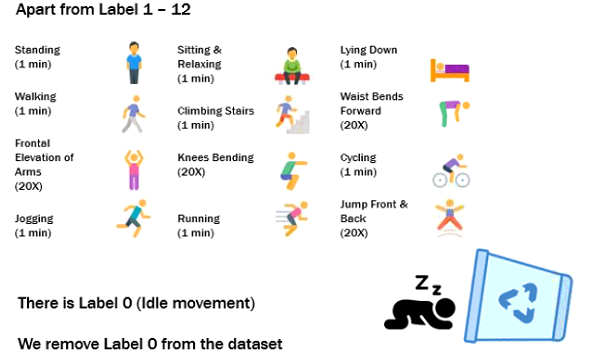
\includegraphics{img/datacleaning.png}
\caption{title}
\end{figure}

    \begin{Verbatim}[commandchars=\\\{\}]
{\color{incolor}In [{\color{incolor}11}]:} \PY{n}{master}\PY{o}{.}\PY{n}{data\PYZus{}cleaning}\PY{p}{(}\PY{p}{)}
\end{Verbatim}


    \begin{Verbatim}[commandchars=\\\{\}]
before cleaning [ 0  1  2  3  4  6  7  8  9 10 11 12  5]
after cleaning [ 1  2  3  4  6  7  8  9 10 11 12  5]

    \end{Verbatim}

    \begin{Verbatim}[commandchars=\\\{\}]
{\color{incolor}In [{\color{incolor}12}]:} \PY{n}{test}\PY{o}{.}\PY{n}{data\PYZus{}cleaning}\PY{p}{(}\PY{p}{)}
\end{Verbatim}


    \begin{Verbatim}[commandchars=\\\{\}]
before cleaning [ 0  1  2  3  4  6  7  8  9 10 11 12  5]
after cleaning [ 1  2  3  4  6  7  8  9 10 11 12  5]

    \end{Verbatim}

    \section{Dataset Description}\label{dataset-description}

    \begin{enumerate}
\def\labelenumi{\arabic{enumi})}
\setcounter{enumi}{1}
\tightlist
\item
  Activity set
\end{enumerate}

The activity set is listed in the following:

L1: Standing still (1 min) L2: Sitting and relaxing (1 min) L3: Lying
down (1 min) L4: Walking (1 min) L5: Climbing stairs (1 min) L6: Waist
bends forward (20x) L7: Frontal elevation of arms (20x) L8: Knees
bending (crouching) (20x) L9: Cycling (1 min) L10: Jogging (1 min) L11:
Running (1 min) L12: Jump front \& back (20x)

    \section{masterset and testset rows and columns are as
follows:}\label{masterset-and-testset-rows-and-columns-are-as-follows}

\subsubsection{25 columns, 23 are
features}\label{columns-23-are-features}

\subsubsection{Label = subjects movement}\label{label-subjects-movement}

\subsubsection{subject = subject
identity}\label{subject-subject-identity}

    \begin{figure}
\centering
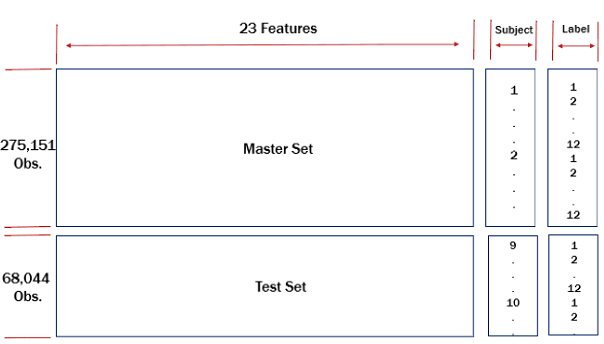
\includegraphics{img/datadescription.png}
\caption{title}
\end{figure}

    \section{The code to get dataset descriptive figures is as
follows}\label{the-code-to-get-dataset-descriptive-figures-is-as-follows}

    \section{Master and test datasets
size}\label{master-and-test-datasets-size}

    \begin{Verbatim}[commandchars=\\\{\}]
{\color{incolor}In [{\color{incolor}13}]:} \PY{n}{master}\PY{o}{.}\PY{n}{get\PYZus{}data}\PY{p}{(}\PY{p}{)}\PY{o}{.}\PY{n}{shape}
\end{Verbatim}


\begin{Verbatim}[commandchars=\\\{\}]
{\color{outcolor}Out[{\color{outcolor}13}]:} (275151, 25)
\end{Verbatim}
            
    \begin{Verbatim}[commandchars=\\\{\}]
{\color{incolor}In [{\color{incolor}14}]:} \PY{n}{test}\PY{o}{.}\PY{n}{get\PYZus{}data}\PY{p}{(}\PY{p}{)}\PY{o}{.}\PY{n}{shape}
\end{Verbatim}


\begin{Verbatim}[commandchars=\\\{\}]
{\color{outcolor}Out[{\color{outcolor}14}]:} (68044, 25)
\end{Verbatim}
            
    \section{Original features in master and test
sets}\label{original-features-in-master-and-test-sets}

    \begin{Verbatim}[commandchars=\\\{\}]
{\color{incolor}In [{\color{incolor}15}]:} \PY{n}{master}\PY{o}{.}\PY{n}{get\PYZus{}data}\PY{p}{(}\PY{p}{)}\PY{o}{.}\PY{n}{columns}
\end{Verbatim}


\begin{Verbatim}[commandchars=\\\{\}]
{\color{outcolor}Out[{\color{outcolor}15}]:} Index(['AccelerationChestX', 'AccelerationChestY', 'AccelerationChestZ',
                'ElectrocardiogramLead1', 'ElectrocardiogramLead2',
                'AccelerationAnkleX', 'AccelerationAnkleY', 'AccelerationAnkleZ',
                'GyroAnkleX', 'GyroAnkleY', 'GyroAnkleZ', 'MagnetometerAnkleX',
                'MagnetometerAnkleY', 'MagnetometerAnkleZ', 'AccelerationArmX',
                'AccelerationArmY', 'AccelerationArmZ', 'GyroArmX', 'GyroArmY',
                'GyroArmZ', 'MagnetometerArmX', 'MagnetometerArmY', 'MagnetometerArmZ',
                'Label', 'Subject'],
               dtype='object')
\end{Verbatim}
            
    \section{You can select any variables you want as features (Label and
Subject columns must be included). All original features in XYZ as well
as Label and Subject are selected in our
case}\label{you-can-select-any-variables-you-want-as-features-label-and-subject-columns-must-be-included.-all-original-features-in-xyz-as-well-as-label-and-subject-are-selected-in-our-case}

    \begin{Verbatim}[commandchars=\\\{\}]
{\color{incolor}In [{\color{incolor}16}]:} \PY{n}{master}\PY{o}{.}\PY{n}{data\PYZus{}selected\PYZus{}features}\PY{p}{(}\PY{p}{[}\PY{l+s+s1}{\PYZsq{}}\PY{l+s+s1}{Label}\PY{l+s+s1}{\PYZsq{}}\PY{p}{,} \PY{l+s+s1}{\PYZsq{}}\PY{l+s+s1}{Subject}\PY{l+s+s1}{\PYZsq{}}\PY{p}{,}\PY{l+s+s1}{\PYZsq{}}\PY{l+s+s1}{AccelerationChestX}\PY{l+s+s1}{\PYZsq{}}\PY{p}{,} \PY{l+s+s1}{\PYZsq{}}\PY{l+s+s1}{AccelerationChestY}\PY{l+s+s1}{\PYZsq{}}\PY{p}{,} \PY{l+s+s1}{\PYZsq{}}\PY{l+s+s1}{AccelerationChestZ}\PY{l+s+s1}{\PYZsq{}}\PY{p}{,}
                \PY{l+s+s1}{\PYZsq{}}\PY{l+s+s1}{ElectrocardiogramLead1}\PY{l+s+s1}{\PYZsq{}}\PY{p}{,} \PY{l+s+s1}{\PYZsq{}}\PY{l+s+s1}{ElectrocardiogramLead2}\PY{l+s+s1}{\PYZsq{}}\PY{p}{,}
                \PY{l+s+s1}{\PYZsq{}}\PY{l+s+s1}{AccelerationAnkleX}\PY{l+s+s1}{\PYZsq{}}\PY{p}{,} \PY{l+s+s1}{\PYZsq{}}\PY{l+s+s1}{AccelerationAnkleY}\PY{l+s+s1}{\PYZsq{}}\PY{p}{,} \PY{l+s+s1}{\PYZsq{}}\PY{l+s+s1}{AccelerationAnkleZ}\PY{l+s+s1}{\PYZsq{}}\PY{p}{,}
                \PY{l+s+s1}{\PYZsq{}}\PY{l+s+s1}{GyroAnkleX}\PY{l+s+s1}{\PYZsq{}}\PY{p}{,} \PY{l+s+s1}{\PYZsq{}}\PY{l+s+s1}{GyroAnkleY}\PY{l+s+s1}{\PYZsq{}}\PY{p}{,} \PY{l+s+s1}{\PYZsq{}}\PY{l+s+s1}{GyroAnkleZ}\PY{l+s+s1}{\PYZsq{}}\PY{p}{,} \PY{l+s+s1}{\PYZsq{}}\PY{l+s+s1}{MagnetometerAnkleX}\PY{l+s+s1}{\PYZsq{}}\PY{p}{,}
                \PY{l+s+s1}{\PYZsq{}}\PY{l+s+s1}{MagnetometerAnkleY}\PY{l+s+s1}{\PYZsq{}}\PY{p}{,} \PY{l+s+s1}{\PYZsq{}}\PY{l+s+s1}{MagnetometerAnkleZ}\PY{l+s+s1}{\PYZsq{}}\PY{p}{,} \PY{l+s+s1}{\PYZsq{}}\PY{l+s+s1}{AccelerationArmX}\PY{l+s+s1}{\PYZsq{}}\PY{p}{,}
                \PY{l+s+s1}{\PYZsq{}}\PY{l+s+s1}{AccelerationArmY}\PY{l+s+s1}{\PYZsq{}}\PY{p}{,} \PY{l+s+s1}{\PYZsq{}}\PY{l+s+s1}{AccelerationArmZ}\PY{l+s+s1}{\PYZsq{}}\PY{p}{,} \PY{l+s+s1}{\PYZsq{}}\PY{l+s+s1}{GyroArmX}\PY{l+s+s1}{\PYZsq{}}\PY{p}{,} \PY{l+s+s1}{\PYZsq{}}\PY{l+s+s1}{GyroArmY}\PY{l+s+s1}{\PYZsq{}}\PY{p}{,}
                \PY{l+s+s1}{\PYZsq{}}\PY{l+s+s1}{GyroArmZ}\PY{l+s+s1}{\PYZsq{}}\PY{p}{,} \PY{l+s+s1}{\PYZsq{}}\PY{l+s+s1}{MagnetometerArmX}\PY{l+s+s1}{\PYZsq{}}\PY{p}{,} \PY{l+s+s1}{\PYZsq{}}\PY{l+s+s1}{MagnetometerArmY}\PY{l+s+s1}{\PYZsq{}}\PY{p}{,} \PY{l+s+s1}{\PYZsq{}}\PY{l+s+s1}{MagnetometerArmZ}\PY{l+s+s1}{\PYZsq{}}
                \PY{p}{]}\PY{p}{)}
\end{Verbatim}


    \begin{Verbatim}[commandchars=\\\{\}]
before features selected Index(['AccelerationChestX', 'AccelerationChestY', 'AccelerationChestZ',
       'ElectrocardiogramLead1', 'ElectrocardiogramLead2',
       'AccelerationAnkleX', 'AccelerationAnkleY', 'AccelerationAnkleZ',
       'GyroAnkleX', 'GyroAnkleY', 'GyroAnkleZ', 'MagnetometerAnkleX',
       'MagnetometerAnkleY', 'MagnetometerAnkleZ', 'AccelerationArmX',
       'AccelerationArmY', 'AccelerationArmZ', 'GyroArmX', 'GyroArmY',
       'GyroArmZ', 'MagnetometerArmX', 'MagnetometerArmY', 'MagnetometerArmZ',
       'Label', 'Subject'],
      dtype='object')
after features selected Index(['Label', 'Subject', 'AccelerationChestX', 'AccelerationChestY',
       'AccelerationChestZ', 'ElectrocardiogramLead1',
       'ElectrocardiogramLead2', 'AccelerationAnkleX', 'AccelerationAnkleY',
       'AccelerationAnkleZ', 'GyroAnkleX', 'GyroAnkleY', 'GyroAnkleZ',
       'MagnetometerAnkleX', 'MagnetometerAnkleY', 'MagnetometerAnkleZ',
       'AccelerationArmX', 'AccelerationArmY', 'AccelerationArmZ', 'GyroArmX',
       'GyroArmY', 'GyroArmZ', 'MagnetometerArmX', 'MagnetometerArmY',
       'MagnetometerArmZ'],
      dtype='object')

    \end{Verbatim}

    \begin{Verbatim}[commandchars=\\\{\}]
{\color{incolor}In [{\color{incolor}17}]:} \PY{n}{test}\PY{o}{.}\PY{n}{data\PYZus{}selected\PYZus{}features}\PY{p}{(}\PY{p}{[}\PY{l+s+s1}{\PYZsq{}}\PY{l+s+s1}{Label}\PY{l+s+s1}{\PYZsq{}}\PY{p}{,} \PY{l+s+s1}{\PYZsq{}}\PY{l+s+s1}{Subject}\PY{l+s+s1}{\PYZsq{}}\PY{p}{,}\PY{l+s+s1}{\PYZsq{}}\PY{l+s+s1}{AccelerationChestX}\PY{l+s+s1}{\PYZsq{}}\PY{p}{,} \PY{l+s+s1}{\PYZsq{}}\PY{l+s+s1}{AccelerationChestY}\PY{l+s+s1}{\PYZsq{}}\PY{p}{,} \PY{l+s+s1}{\PYZsq{}}\PY{l+s+s1}{AccelerationChestZ}\PY{l+s+s1}{\PYZsq{}}\PY{p}{,}
                \PY{l+s+s1}{\PYZsq{}}\PY{l+s+s1}{ElectrocardiogramLead1}\PY{l+s+s1}{\PYZsq{}}\PY{p}{,} \PY{l+s+s1}{\PYZsq{}}\PY{l+s+s1}{ElectrocardiogramLead2}\PY{l+s+s1}{\PYZsq{}}\PY{p}{,}
                \PY{l+s+s1}{\PYZsq{}}\PY{l+s+s1}{AccelerationAnkleX}\PY{l+s+s1}{\PYZsq{}}\PY{p}{,} \PY{l+s+s1}{\PYZsq{}}\PY{l+s+s1}{AccelerationAnkleY}\PY{l+s+s1}{\PYZsq{}}\PY{p}{,} \PY{l+s+s1}{\PYZsq{}}\PY{l+s+s1}{AccelerationAnkleZ}\PY{l+s+s1}{\PYZsq{}}\PY{p}{,}
                \PY{l+s+s1}{\PYZsq{}}\PY{l+s+s1}{GyroAnkleX}\PY{l+s+s1}{\PYZsq{}}\PY{p}{,} \PY{l+s+s1}{\PYZsq{}}\PY{l+s+s1}{GyroAnkleY}\PY{l+s+s1}{\PYZsq{}}\PY{p}{,} \PY{l+s+s1}{\PYZsq{}}\PY{l+s+s1}{GyroAnkleZ}\PY{l+s+s1}{\PYZsq{}}\PY{p}{,} \PY{l+s+s1}{\PYZsq{}}\PY{l+s+s1}{MagnetometerAnkleX}\PY{l+s+s1}{\PYZsq{}}\PY{p}{,}
                \PY{l+s+s1}{\PYZsq{}}\PY{l+s+s1}{MagnetometerAnkleY}\PY{l+s+s1}{\PYZsq{}}\PY{p}{,} \PY{l+s+s1}{\PYZsq{}}\PY{l+s+s1}{MagnetometerAnkleZ}\PY{l+s+s1}{\PYZsq{}}\PY{p}{,} \PY{l+s+s1}{\PYZsq{}}\PY{l+s+s1}{AccelerationArmX}\PY{l+s+s1}{\PYZsq{}}\PY{p}{,}
                \PY{l+s+s1}{\PYZsq{}}\PY{l+s+s1}{AccelerationArmY}\PY{l+s+s1}{\PYZsq{}}\PY{p}{,} \PY{l+s+s1}{\PYZsq{}}\PY{l+s+s1}{AccelerationArmZ}\PY{l+s+s1}{\PYZsq{}}\PY{p}{,} \PY{l+s+s1}{\PYZsq{}}\PY{l+s+s1}{GyroArmX}\PY{l+s+s1}{\PYZsq{}}\PY{p}{,} \PY{l+s+s1}{\PYZsq{}}\PY{l+s+s1}{GyroArmY}\PY{l+s+s1}{\PYZsq{}}\PY{p}{,}
                \PY{l+s+s1}{\PYZsq{}}\PY{l+s+s1}{GyroArmZ}\PY{l+s+s1}{\PYZsq{}}\PY{p}{,} \PY{l+s+s1}{\PYZsq{}}\PY{l+s+s1}{MagnetometerArmX}\PY{l+s+s1}{\PYZsq{}}\PY{p}{,} \PY{l+s+s1}{\PYZsq{}}\PY{l+s+s1}{MagnetometerArmY}\PY{l+s+s1}{\PYZsq{}}\PY{p}{,} \PY{l+s+s1}{\PYZsq{}}\PY{l+s+s1}{MagnetometerArmZ}\PY{l+s+s1}{\PYZsq{}}
                \PY{p}{]}\PY{p}{)}
\end{Verbatim}


    \begin{Verbatim}[commandchars=\\\{\}]
before features selected Index(['AccelerationChestX', 'AccelerationChestY', 'AccelerationChestZ',
       'ElectrocardiogramLead1', 'ElectrocardiogramLead2',
       'AccelerationAnkleX', 'AccelerationAnkleY', 'AccelerationAnkleZ',
       'GyroAnkleX', 'GyroAnkleY', 'GyroAnkleZ', 'MagnetometerAnkleX',
       'MagnetometerAnkleY', 'MagnetometerAnkleZ', 'AccelerationArmX',
       'AccelerationArmY', 'AccelerationArmZ', 'GyroArmX', 'GyroArmY',
       'GyroArmZ', 'MagnetometerArmX', 'MagnetometerArmY', 'MagnetometerArmZ',
       'Label', 'Subject'],
      dtype='object')
after features selected Index(['Label', 'Subject', 'AccelerationChestX', 'AccelerationChestY',
       'AccelerationChestZ', 'ElectrocardiogramLead1',
       'ElectrocardiogramLead2', 'AccelerationAnkleX', 'AccelerationAnkleY',
       'AccelerationAnkleZ', 'GyroAnkleX', 'GyroAnkleY', 'GyroAnkleZ',
       'MagnetometerAnkleX', 'MagnetometerAnkleY', 'MagnetometerAnkleZ',
       'AccelerationArmX', 'AccelerationArmY', 'AccelerationArmZ', 'GyroArmX',
       'GyroArmY', 'GyroArmZ', 'MagnetometerArmX', 'MagnetometerArmY',
       'MagnetometerArmZ'],
      dtype='object')

    \end{Verbatim}

    \section{First 5 observations of master and test
sets}\label{first-5-observations-of-master-and-test-sets}

    \begin{Verbatim}[commandchars=\\\{\}]
{\color{incolor}In [{\color{incolor}18}]:} \PY{n}{master}\PY{o}{.}\PY{n}{get\PYZus{}data}\PY{p}{(}\PY{p}{)}\PY{o}{.}\PY{n}{head}\PY{p}{(}\PY{p}{)}
\end{Verbatim}


\begin{Verbatim}[commandchars=\\\{\}]
{\color{outcolor}Out[{\color{outcolor}18}]:}       Label  Subject  AccelerationChestX  AccelerationChestY  \textbackslash{}
         6656      1        1             -9.7788             0.55690   
         6657      1        1             -9.7733             0.27880   
         6658      1        1             -9.8609             0.11561   
         6659      1        1             -9.7409             0.17652   
         6660      1        1             -9.7821             0.21637   
         
               AccelerationChestZ  ElectrocardiogramLead1  ElectrocardiogramLead2  \textbackslash{}
         6656             1.19750                0.008373               -0.033490   
         6657             0.73036               -0.025118               -0.025118   
         6658             0.79988                0.025118                0.016745   
         6659             0.88957                0.180010                0.129770   
         6660             0.90368                0.092098                0.046049   
         
               AccelerationAnkleX  AccelerationAnkleY  AccelerationAnkleZ  \textbackslash{}
         6656              2.6493             -9.4517             0.37683   
         6657              2.4157             -9.5306             0.40179   
         6658              2.3865             -9.5991             0.48141   
         6659              2.3758             -9.5997             0.42919   
         6660              2.3239             -9.5406             0.40038   
         
                     {\ldots}         MagnetometerAnkleZ  AccelerationArmX  \textbackslash{}
         6656        {\ldots}                   -0.73822           -2.8439   
         6657        {\ldots}                   -0.88628           -2.9935   
         6658        {\ldots}                   -1.01980           -2.8846   
         6659        {\ldots}                   -1.17150           -2.9245   
         6660        {\ldots}                   -0.88628           -2.8963   
         
               AccelerationArmY  AccelerationArmZ  GyroArmX  GyroArmY  GyroArmZ  \textbackslash{}
         6656           -9.0618            1.8177 -0.058824  -0.93429  -0.34483   
         6657           -9.2048            1.5189 -0.058824  -0.93429  -0.34483   
         6658           -9.1945            1.5507 -0.058824  -0.93429  -0.34483   
         6659           -9.1746            1.5413 -0.078431  -0.93429  -0.34052   
         6660           -9.2039            1.6127 -0.078431  -0.93429  -0.34052   
         
               MagnetometerArmX  MagnetometerArmY  MagnetometerArmZ  
         6656          0.355370          -0.37003          -0.35020  
         6657          0.719910           0.17803           0.37363  
         6658          0.355370          -0.37003          -0.35020  
         6659          0.357180          -0.18858          -0.35198  
         6660         -0.001887          -0.18867          -0.72017  
         
         [5 rows x 25 columns]
\end{Verbatim}
            
    \begin{Verbatim}[commandchars=\\\{\}]
{\color{incolor}In [{\color{incolor}19}]:} \PY{n}{test}\PY{o}{.}\PY{n}{get\PYZus{}data}\PY{p}{(}\PY{p}{)}\PY{o}{.}\PY{n}{head}\PY{p}{(}\PY{p}{)}
\end{Verbatim}


\begin{Verbatim}[commandchars=\\\{\}]
{\color{outcolor}Out[{\color{outcolor}19}]:}        Label  Subject  AccelerationChestX  AccelerationChestY  \textbackslash{}
         12288      1        9             -9.4805             -1.7301   
         12289      1        9             -9.4886             -1.8315   
         12290      1        9             -9.9525             -1.8703   
         12291      1        9             -9.5801             -1.8014   
         12292      1        9             -9.2542             -1.9377   
         
                AccelerationChestZ  ElectrocardiogramLead1  ElectrocardiogramLead2  \textbackslash{}
         12288            -0.10308               -0.753530               -0.502350   
         12289            -0.08062               -0.288850               -0.125590   
         12290             0.30536               -0.041863               -0.004186   
         12291            -0.15160                0.025118                0.037677   
         12292            -0.33229                0.092098                0.092098   
         
                AccelerationAnkleX  AccelerationAnkleY  AccelerationAnkleZ  \textbackslash{}
         12288             0.79065             -9.7829             0.91459   
         12289             0.80350             -9.9303             1.03240   
         12290             0.71974             -9.7724             0.97691   
         12291             0.75194             -9.9608             0.94698   
         12292             0.73087             -9.8915             0.95023   
         
                      {\ldots}         MagnetometerAnkleZ  AccelerationArmX  \textbackslash{}
         12288        {\ldots}                   -0.44769           -2.7267   
         12289        {\ldots}                   -0.58122           -2.7424   
         12290        {\ldots}                   -0.29787           -2.7871   
         12291        {\ldots}                   -0.58481           -2.9003   
         12292        {\ldots}                   -0.44410           -2.9607   
         
                AccelerationArmY  AccelerationArmZ  GyroArmX  GyroArmY  GyroArmZ  \textbackslash{}
         12288           -9.0376            1.2356  -0.80784  -0.70226  -0.15302   
         12289           -9.3879            1.2077  -0.80784  -0.70226  -0.15302   
         12290           -8.9777            1.2282  -0.80784  -0.68994  -0.15948   
         12291           -9.2391            1.0901  -0.80784  -0.68994  -0.15948   
         12292           -9.2091            1.0916  -0.80784  -0.68994  -0.15948   
         
                MagnetometerArmX  MagnetometerArmY  MagnetometerArmZ  
         12288          0.008892           0.88921           -1.8138  
         12289         -0.174250           0.52807           -1.8138  
         12290          0.366180           0.71146           -1.0828  
         12291          0.188370           0.88385           -2.1711  
         12292          0.369740           1.06710           -1.8083  
         
         [5 rows x 25 columns]
\end{Verbatim}
            
    \section{Brief descriptive figures of master and test
sets}\label{brief-descriptive-figures-of-master-and-test-sets}

    \begin{Verbatim}[commandchars=\\\{\}]
{\color{incolor}In [{\color{incolor}20}]:} \PY{n}{master}\PY{o}{.}\PY{n}{get\PYZus{}data}\PY{p}{(}\PY{p}{)}\PY{o}{.}\PY{n}{describe}\PY{p}{(}\PY{p}{)}
\end{Verbatim}


\begin{Verbatim}[commandchars=\\\{\}]
{\color{outcolor}Out[{\color{outcolor}20}]:}                Label        Subject  AccelerationChestX  AccelerationChestY  \textbackslash{}
         count  275151.000000  275151.000000       275151.000000       275151.000000   
         mean        6.169147       4.445130           -7.521110           -0.143850   
         std         3.294922       2.290791            5.756336            2.642278   
         min         1.000000       1.000000          -22.438000          -20.188000   
         25\%         3.000000       2.000000           -9.730100           -1.188600   
         50\%         6.000000       4.000000           -8.831800           -0.290240   
         75\%         9.000000       6.000000           -5.347200            0.875830   
         max        12.000000       8.000000           19.094000           20.917000   
         
                AccelerationChestZ  ElectrocardiogramLead1  ElectrocardiogramLead2  \textbackslash{}
         count       275151.000000           275151.000000           275151.000000   
         mean            -0.699136                0.000503               -0.010255   
         std              4.635464                0.902349                0.931583   
         min            -18.401000               -8.619600               -8.619600   
         25\%             -3.463450               -0.230250               -0.188380   
         50\%             -0.642570               -0.075353               -0.050235   
         75\%              1.360550                0.175820                0.154890   
         max             26.196000                8.506500                8.519100   
         
                AccelerationAnkleX  AccelerationAnkleY  AccelerationAnkleZ  \textbackslash{}
         count       275151.000000       275151.000000       275151.000000   
         mean             1.812238           -9.061107           -0.719000   
         std              4.156885            5.181774            6.451024   
         min            -22.146000          -19.619000          -19.373000   
         25\%              0.133210          -10.067000           -3.464600   
         50\%              1.449700           -9.585400            0.290490   
         75\%              2.927250           -7.490700            1.811800   
         max             20.024000           21.161000           25.015000   
         
                      {\ldots}         MagnetometerAnkleZ  AccelerationArmX  \textbackslash{}
         count        {\ldots}              275151.000000     275151.000000   
         mean         {\ldots}                  -0.290972         -3.304465   
         std          {\ldots}                  19.615009          5.937592   
         min          {\ldots}                -282.390000        -22.345000   
         25\%          {\ldots}                  -1.798300         -4.897050   
         50\%          {\ldots}                  -0.297870         -2.300900   
         75\%          {\ldots}                   1.553900         -0.388945   
         max          {\ldots}                 272.560000         19.801000   
         
                AccelerationArmY  AccelerationArmZ       GyroArmX       GyroArmY  \textbackslash{}
         count     275151.000000     275151.000000  275151.000000  275151.000000   
         mean          -5.836086          2.453024      -0.208735      -0.397540   
         std            6.613616          4.288466       0.539642       0.557495   
         min          -18.972000        -18.238000      -1.170600      -2.205300   
         25\%           -9.587100          0.353010      -0.641180      -0.833680   
         50\%           -7.748900          1.999100      -0.294120      -0.593430   
         75\%           -2.181600          5.234500       0.186270      -0.022587   
         max           21.965000         25.741000       1.321600       1.121100   
         
                     GyroArmZ  MagnetometerArmX  MagnetometerArmY  MagnetometerArmZ  
         count  275151.000000     275151.000000     275151.000000     275151.000000  
         mean        0.379569         -0.507261          1.569891          0.379133  
         std         0.519960         34.443681         31.853086         84.864603  
         min        -1.114200       -319.030000       -358.130000       -702.570000  
         25\%        -0.038793         -6.714850         -7.694150        -12.552000  
         50\%         0.454740          0.358960          0.353650         -0.494730  
         75\%         0.844830          5.524700          9.265950         11.233000  
         max         1.528000        234.890000        335.250000        657.180000  
         
         [8 rows x 25 columns]
\end{Verbatim}
            
    \begin{Verbatim}[commandchars=\\\{\}]
{\color{incolor}In [{\color{incolor}21}]:} \PY{n}{test}\PY{o}{.}\PY{n}{get\PYZus{}data}\PY{p}{(}\PY{p}{)}\PY{o}{.}\PY{n}{describe}\PY{p}{(}\PY{p}{)}
\end{Verbatim}


\begin{Verbatim}[commandchars=\\\{\}]
{\color{outcolor}Out[{\color{outcolor}21}]:}               Label       Subject  AccelerationChestX  AccelerationChestY  \textbackslash{}
         count  68044.000000  68044.000000        68044.000000        68044.000000   
         mean       6.168509      9.495121           -7.340349           -0.129089   
         std        3.314973      0.499980            5.474165            3.360574   
         min        1.000000      9.000000          -22.296000          -20.021000   
         25\%        3.000000      9.000000           -9.619900           -1.883100   
         50\%        6.000000      9.000000           -8.583500           -0.303405   
         75\%        9.000000     10.000000           -4.636675            1.809825   
         max       12.000000     10.000000           17.618000           20.927000   
         
                AccelerationChestZ  ElectrocardiogramLead1  ElectrocardiogramLead2  \textbackslash{}
         count        68044.000000            68044.000000            68044.000000   
         mean            -1.906006                0.016370                0.000879   
         std              4.380268                0.508203                0.448549   
         min            -18.400000               -3.604400               -4.600700   
         25\%             -4.736775               -0.159080               -0.125590   
         50\%             -1.813650               -0.066981               -0.046049   
         75\%              0.131322                0.129770                0.092098   
         max             10.562000                4.081600                4.684500   
         
                AccelerationAnkleX  AccelerationAnkleY  AccelerationAnkleZ  \textbackslash{}
         count        68044.000000        68044.000000        68044.000000   
         mean             1.776662           -9.063023           -0.633180   
         std              4.438221            5.275032            6.483828   
         min            -22.126000          -19.599000          -19.364000   
         25\%              0.226148          -10.052000           -3.582025   
         50\%              0.967950           -9.671100            0.487160   
         75\%              2.874200           -8.123975            1.930425   
         max             20.014000           20.766000           24.400000   
         
                      {\ldots}         MagnetometerAnkleZ  AccelerationArmX  \textbackslash{}
         count        {\ldots}               68044.000000      68044.000000   
         mean         {\ldots}                  -0.739776         -4.029430   
         std          {\ldots}                  15.665477          5.664786   
         min          {\ldots}                -203.550000        -21.905000   
         25\%          {\ldots}                  -1.614625         -5.687100   
         50\%          {\ldots}                  -0.442260         -2.927200   
         75\%          {\ldots}                   1.624225         -1.532300   
         max          {\ldots}                 179.730000         19.398000   
         
                AccelerationArmY  AccelerationArmZ      GyroArmX      GyroArmY  \textbackslash{}
         count      68044.000000      68044.000000  68044.000000  68044.000000   
         mean          -5.560494          2.090584     -0.172617     -0.462985   
         std            6.429193          3.683399      0.586904      0.495348   
         min          -18.928000        -18.216000     -1.060800     -2.256700   
         25\%           -9.460075         -0.231200     -0.729410     -0.788500   
         50\%           -7.700900          1.052400     -0.386270     -0.613960   
         75\%           -2.422575          5.865700      0.409800     -0.123200   
         max           21.807000         23.974000      1.415700      0.683780   
         
                    GyroArmZ  MagnetometerArmX  MagnetometerArmY  MagnetometerArmZ  
         count  68044.000000      68044.000000      68044.000000      68044.000000  
         mean       0.385237         -0.635213          0.824676         -1.378418  
         std        0.497859         33.280826         22.865112         73.070786  
         min       -0.870690       -207.920000       -316.230000       -504.800000  
         25\%       -0.045259         -4.776800         -5.981300        -10.993000  
         50\%        0.443970          0.362620          0.355690         -0.716510  
         75\%        0.814660          4.213200          5.683050          7.157325  
         max        1.377200        239.690000        221.010000        586.080000  
         
         [8 rows x 25 columns]
\end{Verbatim}
            
    \section{12 Actions are included in the
datasets}\label{actions-are-included-in-the-datasets}

    \begin{Verbatim}[commandchars=\\\{\}]
{\color{incolor}In [{\color{incolor}22}]:} \PY{n}{master}\PY{o}{.}\PY{n}{get\PYZus{}selected\PYZus{}labels}\PY{p}{(}\PY{p}{)}
\end{Verbatim}


\begin{Verbatim}[commandchars=\\\{\}]
{\color{outcolor}Out[{\color{outcolor}22}]:} array([ 1,  2,  3,  4,  6,  7,  8,  9, 10, 11, 12,  5], dtype=int64)
\end{Verbatim}
            
    \begin{Verbatim}[commandchars=\\\{\}]
{\color{incolor}In [{\color{incolor}23}]:} \PY{n}{test}\PY{o}{.}\PY{n}{get\PYZus{}selected\PYZus{}labels}\PY{p}{(}\PY{p}{)}
\end{Verbatim}


\begin{Verbatim}[commandchars=\\\{\}]
{\color{outcolor}Out[{\color{outcolor}23}]:} array([ 1,  2,  3,  4,  6,  7,  8,  9, 10, 11, 12,  5], dtype=int64)
\end{Verbatim}
            
    \begin{Verbatim}[commandchars=\\\{\}]
{\color{incolor}In [{\color{incolor}24}]:} \PY{n+nb}{print}\PY{p}{(}\PY{n}{master}\PY{o}{.}\PY{n}{get\PYZus{}data}\PY{p}{(}\PY{p}{)}\PY{o}{.}\PY{n}{shape}\PY{p}{)}
         \PY{n+nb}{print}\PY{p}{(}\PY{n}{test}\PY{o}{.}\PY{n}{get\PYZus{}data}\PY{p}{(}\PY{p}{)}\PY{o}{.}\PY{n}{shape}\PY{p}{)}
\end{Verbatim}


    \begin{Verbatim}[commandchars=\\\{\}]
(275151, 25)
(68044, 25)

    \end{Verbatim}

    \begin{Verbatim}[commandchars=\\\{\}]
{\color{incolor}In [{\color{incolor}25}]:} \PY{n+nb}{len}\PY{p}{(}\PY{n}{master}\PY{o}{.}\PY{n}{get\PYZus{}selected\PYZus{}labels}\PY{p}{(}\PY{p}{)}\PY{p}{)}
\end{Verbatim}


\begin{Verbatim}[commandchars=\\\{\}]
{\color{outcolor}Out[{\color{outcolor}25}]:} 12
\end{Verbatim}
            
    \section{Number of observations of 12 actions for subject 9 and
10}\label{number-of-observations-of-12-actions-for-subject-9-and-10}

    \begin{Verbatim}[commandchars=\\\{\}]
{\color{incolor}In [{\color{incolor}26}]:} \PY{n}{test}\PY{o}{.}\PY{n}{get\PYZus{}data}\PY{p}{(}\PY{p}{)}\PY{o}{.}\PY{n}{groupby}\PY{p}{(}\PY{n}{by} \PY{o}{=} \PY{p}{[}\PY{l+s+s1}{\PYZsq{}}\PY{l+s+s1}{Subject}\PY{l+s+s1}{\PYZsq{}}\PY{p}{,}\PY{l+s+s1}{\PYZsq{}}\PY{l+s+s1}{Label}\PY{l+s+s1}{\PYZsq{}}\PY{p}{]}\PY{p}{)}\PY{o}{.}\PY{n}{count}\PY{p}{(}\PY{p}{)}
\end{Verbatim}


\begin{Verbatim}[commandchars=\\\{\}]
{\color{outcolor}Out[{\color{outcolor}26}]:}                AccelerationChestX  AccelerationChestY  AccelerationChestZ  \textbackslash{}
         Subject Label                                                               
         9       1                    3072                3072                3072   
                 2                    3072                3072                3072   
                 3                    3072                3072                3072   
                 4                    3072                3072                3072   
                 5                    3072                3072                3072   
                 6                    2867                2867                2867   
                 7                    2867                2867                2867   
                 8                    2969                2969                2969   
                 9                    3072                3072                3072   
                 10                   3072                3072                3072   
                 11                   3072                3072                3072   
                 12                   1075                1075                1075   
         10      1                    3072                3072                3072   
                 2                    3072                3072                3072   
                 3                    3072                3072                3072   
                 4                    3072                3072                3072   
                 5                    3072                3072                3072   
                 6                    2458                2458                2458   
                 7                    2765                2765                2765   
                 8                    2867                2867                2867   
                 9                    3072                3072                3072   
                 10                   3072                3072                3072   
                 11                   3072                3072                3072   
                 12                   1024                1024                1024   
         
                        ElectrocardiogramLead1  ElectrocardiogramLead2  \textbackslash{}
         Subject Label                                                   
         9       1                        3072                    3072   
                 2                        3072                    3072   
                 3                        3072                    3072   
                 4                        3072                    3072   
                 5                        3072                    3072   
                 6                        2867                    2867   
                 7                        2867                    2867   
                 8                        2969                    2969   
                 9                        3072                    3072   
                 10                       3072                    3072   
                 11                       3072                    3072   
                 12                       1075                    1075   
         10      1                        3072                    3072   
                 2                        3072                    3072   
                 3                        3072                    3072   
                 4                        3072                    3072   
                 5                        3072                    3072   
                 6                        2458                    2458   
                 7                        2765                    2765   
                 8                        2867                    2867   
                 9                        3072                    3072   
                 10                       3072                    3072   
                 11                       3072                    3072   
                 12                       1024                    1024   
         
                        AccelerationAnkleX  AccelerationAnkleY  AccelerationAnkleZ  \textbackslash{}
         Subject Label                                                               
         9       1                    3072                3072                3072   
                 2                    3072                3072                3072   
                 3                    3072                3072                3072   
                 4                    3072                3072                3072   
                 5                    3072                3072                3072   
                 6                    2867                2867                2867   
                 7                    2867                2867                2867   
                 8                    2969                2969                2969   
                 9                    3072                3072                3072   
                 10                   3072                3072                3072   
                 11                   3072                3072                3072   
                 12                   1075                1075                1075   
         10      1                    3072                3072                3072   
                 2                    3072                3072                3072   
                 3                    3072                3072                3072   
                 4                    3072                3072                3072   
                 5                    3072                3072                3072   
                 6                    2458                2458                2458   
                 7                    2765                2765                2765   
                 8                    2867                2867                2867   
                 9                    3072                3072                3072   
                 10                   3072                3072                3072   
                 11                   3072                3072                3072   
                 12                   1024                1024                1024   
         
                        GyroAnkleX  GyroAnkleY        {\ldots}         MagnetometerAnkleZ  \textbackslash{}
         Subject Label                                {\ldots}                              
         9       1            3072        3072        {\ldots}                       3072   
                 2            3072        3072        {\ldots}                       3072   
                 3            3072        3072        {\ldots}                       3072   
                 4            3072        3072        {\ldots}                       3072   
                 5            3072        3072        {\ldots}                       3072   
                 6            2867        2867        {\ldots}                       2867   
                 7            2867        2867        {\ldots}                       2867   
                 8            2969        2969        {\ldots}                       2969   
                 9            3072        3072        {\ldots}                       3072   
                 10           3072        3072        {\ldots}                       3072   
                 11           3072        3072        {\ldots}                       3072   
                 12           1075        1075        {\ldots}                       1075   
         10      1            3072        3072        {\ldots}                       3072   
                 2            3072        3072        {\ldots}                       3072   
                 3            3072        3072        {\ldots}                       3072   
                 4            3072        3072        {\ldots}                       3072   
                 5            3072        3072        {\ldots}                       3072   
                 6            2458        2458        {\ldots}                       2458   
                 7            2765        2765        {\ldots}                       2765   
                 8            2867        2867        {\ldots}                       2867   
                 9            3072        3072        {\ldots}                       3072   
                 10           3072        3072        {\ldots}                       3072   
                 11           3072        3072        {\ldots}                       3072   
                 12           1024        1024        {\ldots}                       1024   
         
                        AccelerationArmX  AccelerationArmY  AccelerationArmZ  GyroArmX  \textbackslash{}
         Subject Label                                                                   
         9       1                  3072              3072              3072      3072   
                 2                  3072              3072              3072      3072   
                 3                  3072              3072              3072      3072   
                 4                  3072              3072              3072      3072   
                 5                  3072              3072              3072      3072   
                 6                  2867              2867              2867      2867   
                 7                  2867              2867              2867      2867   
                 8                  2969              2969              2969      2969   
                 9                  3072              3072              3072      3072   
                 10                 3072              3072              3072      3072   
                 11                 3072              3072              3072      3072   
                 12                 1075              1075              1075      1075   
         10      1                  3072              3072              3072      3072   
                 2                  3072              3072              3072      3072   
                 3                  3072              3072              3072      3072   
                 4                  3072              3072              3072      3072   
                 5                  3072              3072              3072      3072   
                 6                  2458              2458              2458      2458   
                 7                  2765              2765              2765      2765   
                 8                  2867              2867              2867      2867   
                 9                  3072              3072              3072      3072   
                 10                 3072              3072              3072      3072   
                 11                 3072              3072              3072      3072   
                 12                 1024              1024              1024      1024   
         
                        GyroArmY  GyroArmZ  MagnetometerArmX  MagnetometerArmY  \textbackslash{}
         Subject Label                                                           
         9       1          3072      3072              3072              3072   
                 2          3072      3072              3072              3072   
                 3          3072      3072              3072              3072   
                 4          3072      3072              3072              3072   
                 5          3072      3072              3072              3072   
                 6          2867      2867              2867              2867   
                 7          2867      2867              2867              2867   
                 8          2969      2969              2969              2969   
                 9          3072      3072              3072              3072   
                 10         3072      3072              3072              3072   
                 11         3072      3072              3072              3072   
                 12         1075      1075              1075              1075   
         10      1          3072      3072              3072              3072   
                 2          3072      3072              3072              3072   
                 3          3072      3072              3072              3072   
                 4          3072      3072              3072              3072   
                 5          3072      3072              3072              3072   
                 6          2458      2458              2458              2458   
                 7          2765      2765              2765              2765   
                 8          2867      2867              2867              2867   
                 9          3072      3072              3072              3072   
                 10         3072      3072              3072              3072   
                 11         3072      3072              3072              3072   
                 12         1024      1024              1024              1024   
         
                        MagnetometerArmZ  
         Subject Label                    
         9       1                  3072  
                 2                  3072  
                 3                  3072  
                 4                  3072  
                 5                  3072  
                 6                  2867  
                 7                  2867  
                 8                  2969  
                 9                  3072  
                 10                 3072  
                 11                 3072  
                 12                 1075  
         10      1                  3072  
                 2                  3072  
                 3                  3072  
                 4                  3072  
                 5                  3072  
                 6                  2458  
                 7                  2765  
                 8                  2867  
                 9                  3072  
                 10                 3072  
                 11                 3072  
                 12                 1024  
         
         [24 rows x 23 columns]
\end{Verbatim}
            
    \section{Dynamic Time Warping with Feature
Extraction}\label{dynamic-time-warping-with-feature-extraction}

    \section{we will apply two machine learning technqiues (1. scaling and
2. dimension reduction) to master and test set before performing
classification by Dynamic Time
Warping}\label{we-will-apply-two-machine-learning-technqiues-1.-scaling-and-2.-dimension-reduction-to-master-and-test-set-before-performing-classification-by-dynamic-time-warping}

\subsubsection{Scaling = Normalization}\label{scaling-normalization}

\subsubsection{Dimension reduction = Principal Component
Analysis}\label{dimension-reduction-principal-component-analysis}

    \subsubsection{Pass in master and test set to initialize DTW experiment
object}\label{pass-in-master-and-test-set-to-initialize-dtw-experiment-object}

    \begin{Verbatim}[commandchars=\\\{\}]
{\color{incolor}In [{\color{incolor}27}]:} \PY{n}{dtw\PYZus{}experiment} \PY{o}{=} \PY{n}{DTWExperiment}\PY{p}{(}\PY{n}{master}\PY{p}{,} \PY{n}{test}\PY{p}{)}
\end{Verbatim}


    \section{Scaling by Normalization}\label{scaling-by-normalization}

    \subsubsection{As you can see, 23 features have different scales e.g.
max of MagnetoMeterArmX = 234.89 whereas max of GyroArmX =
1.326}\label{as-you-can-see-23-features-have-different-scales-e.g.-max-of-magnetometerarmx-234.89-whereas-max-of-gyroarmx-1.326}

\subsubsection{Machine learning models may have a bias to the features
those are with larger
scales.}\label{machine-learning-models-may-have-a-bias-to-the-features-those-are-with-larger-scales.}

\subsubsection{Therefore, we rescale all 23 features by
normalization}\label{therefore-we-rescale-all-23-features-by-normalization}

    \begin{Verbatim}[commandchars=\\\{\}]
{\color{incolor}In [{\color{incolor}28}]:} \PY{n}{dtw\PYZus{}experiment}\PY{o}{.}\PY{n}{get\PYZus{}masterset}\PY{p}{(}\PY{p}{)}\PY{o}{.}\PY{n}{get\PYZus{}data}\PY{p}{(}\PY{p}{)}\PY{o}{.}\PY{n}{describe}\PY{p}{(}\PY{p}{)}
\end{Verbatim}


\begin{Verbatim}[commandchars=\\\{\}]
{\color{outcolor}Out[{\color{outcolor}28}]:}                Label        Subject  AccelerationChestX  AccelerationChestY  \textbackslash{}
         count  275151.000000  275151.000000       275151.000000       275151.000000   
         mean        6.169147       4.445130           -7.521110           -0.143850   
         std         3.294922       2.290791            5.756336            2.642278   
         min         1.000000       1.000000          -22.438000          -20.188000   
         25\%         3.000000       2.000000           -9.730100           -1.188600   
         50\%         6.000000       4.000000           -8.831800           -0.290240   
         75\%         9.000000       6.000000           -5.347200            0.875830   
         max        12.000000       8.000000           19.094000           20.917000   
         
                AccelerationChestZ  ElectrocardiogramLead1  ElectrocardiogramLead2  \textbackslash{}
         count       275151.000000           275151.000000           275151.000000   
         mean            -0.699136                0.000503               -0.010255   
         std              4.635464                0.902349                0.931583   
         min            -18.401000               -8.619600               -8.619600   
         25\%             -3.463450               -0.230250               -0.188380   
         50\%             -0.642570               -0.075353               -0.050235   
         75\%              1.360550                0.175820                0.154890   
         max             26.196000                8.506500                8.519100   
         
                AccelerationAnkleX  AccelerationAnkleY  AccelerationAnkleZ  \textbackslash{}
         count       275151.000000       275151.000000       275151.000000   
         mean             1.812238           -9.061107           -0.719000   
         std              4.156885            5.181774            6.451024   
         min            -22.146000          -19.619000          -19.373000   
         25\%              0.133210          -10.067000           -3.464600   
         50\%              1.449700           -9.585400            0.290490   
         75\%              2.927250           -7.490700            1.811800   
         max             20.024000           21.161000           25.015000   
         
                      {\ldots}         MagnetometerAnkleZ  AccelerationArmX  \textbackslash{}
         count        {\ldots}              275151.000000     275151.000000   
         mean         {\ldots}                  -0.290972         -3.304465   
         std          {\ldots}                  19.615009          5.937592   
         min          {\ldots}                -282.390000        -22.345000   
         25\%          {\ldots}                  -1.798300         -4.897050   
         50\%          {\ldots}                  -0.297870         -2.300900   
         75\%          {\ldots}                   1.553900         -0.388945   
         max          {\ldots}                 272.560000         19.801000   
         
                AccelerationArmY  AccelerationArmZ       GyroArmX       GyroArmY  \textbackslash{}
         count     275151.000000     275151.000000  275151.000000  275151.000000   
         mean          -5.836086          2.453024      -0.208735      -0.397540   
         std            6.613616          4.288466       0.539642       0.557495   
         min          -18.972000        -18.238000      -1.170600      -2.205300   
         25\%           -9.587100          0.353010      -0.641180      -0.833680   
         50\%           -7.748900          1.999100      -0.294120      -0.593430   
         75\%           -2.181600          5.234500       0.186270      -0.022587   
         max           21.965000         25.741000       1.321600       1.121100   
         
                     GyroArmZ  MagnetometerArmX  MagnetometerArmY  MagnetometerArmZ  
         count  275151.000000     275151.000000     275151.000000     275151.000000  
         mean        0.379569         -0.507261          1.569891          0.379133  
         std         0.519960         34.443681         31.853086         84.864603  
         min        -1.114200       -319.030000       -358.130000       -702.570000  
         25\%        -0.038793         -6.714850         -7.694150        -12.552000  
         50\%         0.454740          0.358960          0.353650         -0.494730  
         75\%         0.844830          5.524700          9.265950         11.233000  
         max         1.528000        234.890000        335.250000        657.180000  
         
         [8 rows x 25 columns]
\end{Verbatim}
            
    \begin{Verbatim}[commandchars=\\\{\}]
{\color{incolor}In [{\color{incolor}29}]:} \PY{n}{dtw\PYZus{}experiment}\PY{o}{.}\PY{n}{get\PYZus{}masterset}\PY{p}{(}\PY{p}{)}\PY{o}{.}\PY{n}{get\PYZus{}data}\PY{p}{(}\PY{p}{)}\PY{o}{.}\PY{n}{describe}\PY{p}{(}\PY{p}{)}\PY{p}{[}\PY{p}{[}\PY{l+s+s1}{\PYZsq{}}\PY{l+s+s1}{GyroArmX}\PY{l+s+s1}{\PYZsq{}}\PY{p}{,}\PY{l+s+s1}{\PYZsq{}}\PY{l+s+s1}{MagnetometerArmX}\PY{l+s+s1}{\PYZsq{}}\PY{p}{]}\PY{p}{]}
\end{Verbatim}


\begin{Verbatim}[commandchars=\\\{\}]
{\color{outcolor}Out[{\color{outcolor}29}]:}             GyroArmX  MagnetometerArmX
         count  275151.000000     275151.000000
         mean       -0.208735         -0.507261
         std         0.539642         34.443681
         min        -1.170600       -319.030000
         25\%        -0.641180         -6.714850
         50\%        -0.294120          0.358960
         75\%         0.186270          5.524700
         max         1.321600        234.890000
\end{Verbatim}
            
    \section{Normalization will be applied in every column individually by
substracting its mean and dividing by its standard deviation (basically
it's z-value), so that all features end up to be in same
scale.}\label{normalization-will-be-applied-in-every-column-individually-by-substracting-its-mean-and-dividing-by-its-standard-deviation-basically-its-z-value-so-that-all-features-end-up-to-be-in-same-scale.}

\subsection{Zij = (Xij -- Mean of Xi) / S.D. of
Xi}\label{zij-xij-mean-of-xi-s.d.-of-xi}

\subsection{For details, please see Method dtw\_experiment.Scaling() and
StandardScaler() in sklearn link
below}\label{for-details-please-see-method-dtw_experiment.scaling-and-standardscaler-in-sklearn-link-below}

\subsection{http://scikit-learn.org/stable/modules/preprocessing.html}\label{httpscikit-learn.orgstablemodulespreprocessing.html}

\subsection{Remarks: you may get confused by the name "Normalization"
and the method StandardScaler() in sklearn. I have no idea why sklearn
named the method as StandardScaler(), but in statistics, we call this as
normalization. So, to be consistent, I think we will just stick to
"Normalization"}\label{remarks-you-may-get-confused-by-the-name-normalization-and-the-method-standardscaler-in-sklearn.-i-have-no-idea-why-sklearn-named-the-method-as-standardscaler-but-in-statistics-we-call-this-as-normalization.-so-to-be-consistent-i-think-we-will-just-stick-to-normalization}

\subsection{https://en.wikipedia.org/wiki/Normalization\_(statistics)}\label{httpsen.wikipedia.orgwikinormalization_statistics}

    \begin{Verbatim}[commandchars=\\\{\}]
{\color{incolor}In [{\color{incolor}30}]:} \PY{n}{dtw\PYZus{}experiment}\PY{o}{.}\PY{n}{restoringDataset}\PY{p}{(}\PY{p}{)}
\end{Verbatim}


    \begin{Verbatim}[commandchars=\\\{\}]
{\color{incolor}In [{\color{incolor}31}]:} \PY{n}{dtw\PYZus{}experiment}\PY{o}{.}\PY{n}{Scaling}\PY{p}{(}\PY{n}{preprocessing}\PY{o}{.}\PY{n}{StandardScaler}\PY{p}{(}\PY{p}{)}\PY{p}{)}
\end{Verbatim}


    \begin{Verbatim}[commandchars=\\\{\}]
(275151, 23)
(275151,)

    \end{Verbatim}

    \section{After rescaling, all 23 features are in same
scale}\label{after-rescaling-all-23-features-are-in-same-scale}

    \begin{Verbatim}[commandchars=\\\{\}]
{\color{incolor}In [{\color{incolor}32}]:} \PY{n}{dtw\PYZus{}experiment}\PY{o}{.}\PY{n}{get\PYZus{}masterset}\PY{p}{(}\PY{p}{)}\PY{o}{.}\PY{n}{get\PYZus{}data}\PY{p}{(}\PY{p}{)}\PY{o}{.}\PY{n}{head}\PY{p}{(}\PY{p}{)}
\end{Verbatim}


\begin{Verbatim}[commandchars=\\\{\}]
{\color{outcolor}Out[{\color{outcolor}32}]:}    AccelerationChestX  AccelerationChestY  AccelerationChestZ  \textbackslash{}
         0           -0.392210            0.265207            0.409158   
         1           -0.391255            0.159957            0.308383   
         2           -0.406473            0.098196            0.323380   
         3           -0.385626            0.121248            0.342729   
         4           -0.392784            0.136330            0.345773   
         
            ElectrocardiogramLead1  ElectrocardiogramLead2  AccelerationAnkleX  \textbackslash{}
         0                0.008721               -0.024941            0.201368   
         1               -0.028394               -0.015954            0.145172   
         2                0.027278                0.028983            0.138148   
         3                0.198933                0.150309            0.135573   
         4                0.101507                0.060439            0.123088   
         
            AccelerationAnkleY  AccelerationAnkleZ  GyroAnkleX  GyroAnkleY  {\ldots}    \textbackslash{}
         0           -0.075378            0.169869   -0.616548   -0.779361  {\ldots}     
         1           -0.090605            0.173739   -0.616548   -0.779361  {\ldots}     
         2           -0.103824            0.186081   -0.596675   -0.732157  {\ldots}     
         3           -0.103940            0.177986   -0.596675   -0.732157  {\ldots}     
         4           -0.092535            0.173520   -0.596675   -0.732157  {\ldots}     
         
            AccelerationArmY  AccelerationArmZ  GyroArmX  GyroArmY  GyroArmZ  \textbackslash{}
         0         -0.487739         -0.148147  0.277797 -0.962791 -1.393183   
         1         -0.509361         -0.217823  0.277797 -0.962791 -1.393183   
         2         -0.507804         -0.210408  0.277797 -0.962791 -1.393183   
         3         -0.504795         -0.212600  0.241463 -0.962791 -1.384894   
         4         -0.509225         -0.195950  0.241463 -0.962791 -1.384894   
         
            MagnetometerArmX  MagnetometerArmY  MagnetometerArmZ  Subject  Label  
         0          0.025045         -0.060902         -0.008594        1      1  
         1          0.035628         -0.043696         -0.000065        1      1  
         2          0.025045         -0.060902         -0.008594        1      1  
         3          0.025097         -0.055206         -0.008615        1      1  
         4          0.014672         -0.055209         -0.012954        1      1  
         
         [5 rows x 25 columns]
\end{Verbatim}
            
    \begin{Verbatim}[commandchars=\\\{\}]
{\color{incolor}In [{\color{incolor}33}]:} \PY{n}{dtw\PYZus{}experiment}\PY{o}{.}\PY{n}{get\PYZus{}testset}\PY{p}{(}\PY{p}{)}\PY{o}{.}\PY{n}{get\PYZus{}data}\PY{p}{(}\PY{p}{)}\PY{o}{.}\PY{n}{head}\PY{p}{(}\PY{p}{)}
\end{Verbatim}


\begin{Verbatim}[commandchars=\\\{\}]
{\color{outcolor}Out[{\color{outcolor}33}]:}    AccelerationChestX  AccelerationChestY  AccelerationChestZ  \textbackslash{}
         0           -0.340389           -0.600335            0.128586   
         1           -0.341796           -0.638711            0.133432   
         2           -0.422386           -0.653396            0.216698   
         3           -0.357692           -0.627320            0.118119   
         4           -0.301076           -0.678904            0.079139   
         
            ElectrocardiogramLead1  ElectrocardiogramLead2  AccelerationAnkleX  \textbackslash{}
         0               -0.835635               -0.528236           -0.245758   
         1               -0.320667               -0.123805           -0.242667   
         2               -0.046951                0.006515           -0.262817   
         3                0.027278                0.051452           -0.255071   
         4                0.101507                0.109870           -0.260139   
         
            AccelerationAnkleY  AccelerationAnkleZ  GyroAnkleX  GyroAnkleY  {\ldots}    \textbackslash{}
         0           -0.139295            0.253230   -1.403181   -0.513315  {\ldots}     
         1           -0.167741            0.271492   -1.403181   -0.513315  {\ldots}     
         2           -0.137268            0.262890   -1.403181   -0.513315  {\ldots}     
         3           -0.173627            0.258251   -1.403181   -0.513315  {\ldots}     
         4           -0.160253            0.258755   -1.359495   -0.491863  {\ldots}     
         
            AccelerationArmY  AccelerationArmZ  GyroArmX  GyroArmY  GyroArmZ  \textbackslash{}
         0         -0.484080         -0.283884 -1.110191 -0.546590 -1.024289   
         1         -0.537047         -0.290390 -1.110191 -0.546590 -1.024289   
         2         -0.475023         -0.285609 -1.110191 -0.524491 -1.036713   
         3         -0.514548         -0.317812 -1.110191 -0.524491 -1.036713   
         4         -0.510011         -0.317462 -1.110191 -0.524491 -1.036713   
         
            MagnetometerArmX  MagnetometerArmY  MagnetometerArmZ  Subject  Label  
         0          0.014985         -0.021369         -0.025840        9      1  
         1          0.009668         -0.032707         -0.025840        9      1  
         2          0.025359         -0.026950         -0.017227        9      1  
         3          0.020196         -0.021538         -0.030051        9      1  
         4          0.025462         -0.015785         -0.025776        9      1  
         
         [5 rows x 25 columns]
\end{Verbatim}
            
    \section{After rescaling, all 23 features are in same scale with zero
mean and one
s.d.}\label{after-rescaling-all-23-features-are-in-same-scale-with-zero-mean-and-one-s.d.}

    \begin{Verbatim}[commandchars=\\\{\}]
{\color{incolor}In [{\color{incolor}34}]:} \PY{n}{pd}\PY{o}{.}\PY{n}{options}\PY{o}{.}\PY{n}{display}\PY{o}{.}\PY{n}{float\PYZus{}format} \PY{o}{=} \PY{l+s+s1}{\PYZsq{}}\PY{l+s+si}{\PYZob{}:,.4f\PYZcb{}}\PY{l+s+s1}{\PYZsq{}}\PY{o}{.}\PY{n}{format}
\end{Verbatim}


    \begin{Verbatim}[commandchars=\\\{\}]
{\color{incolor}In [{\color{incolor}35}]:} \PY{n}{dtw\PYZus{}experiment}\PY{o}{.}\PY{n}{get\PYZus{}masterset}\PY{p}{(}\PY{p}{)}\PY{o}{.}\PY{n}{get\PYZus{}data}\PY{p}{(}\PY{p}{)}\PY{o}{.}\PY{n}{describe}\PY{p}{(}\PY{p}{)}\PY{p}{[}\PY{p}{[}\PY{l+s+s1}{\PYZsq{}}\PY{l+s+s1}{GyroArmX}\PY{l+s+s1}{\PYZsq{}}\PY{p}{,}\PY{l+s+s1}{\PYZsq{}}\PY{l+s+s1}{MagnetometerArmX}\PY{l+s+s1}{\PYZsq{}}\PY{p}{]}\PY{p}{]}
\end{Verbatim}


\begin{Verbatim}[commandchars=\\\{\}]
{\color{outcolor}Out[{\color{outcolor}35}]:}           GyroArmX  MagnetometerArmX
         count 275,151.0000      275,151.0000
         mean       -0.0000           -0.0000
         std         1.0000            1.0000
         min        -1.7824           -9.2477
         25\%        -0.8014           -0.1802
         50\%        -0.1582            0.0251
         75\%         0.7320            0.1751
         max         2.8358            6.8343
\end{Verbatim}
            
    \section{Reducing Dimension by Principal Component
Analysis}\label{reducing-dimension-by-principal-component-analysis}

    \section{Why Dimension Reduction?}\label{why-dimension-reduction}

\subsubsection{- 23 features in our dataset which is too
much}\label{features-in-our-dataset-which-is-too-much}

\subsubsection{- Rule of thumb: Prefer important but small no. of
features rather than unimportant but large no. of
features}\label{rule-of-thumb-prefer-important-but-small-no.-of-features-rather-than-unimportant-but-large-no.-of-features}

\subsubsection{- Curse of dimensionality: Some supervised models such as
multiple linear regression, it has assumptions that the no. of
observations has to be more than no. of
features}\label{curse-of-dimensionality-some-supervised-models-such-as-multiple-linear-regression-it-has-assumptions-that-the-no.-of-observations-has-to-be-more-than-no.-of-features}

\subsubsection{- Collinearity: if Corr(A, B) = 0.99, A is simply equal
to B. Thus, either A or B is
used}\label{collinearity-if-corra-b-0.99-a-is-simply-equal-to-b.-thus-either-a-or-b-is-used}

\subsubsection{- Increase processing
speed}\label{increase-processing-speed}

\subsubsection{https://en.wikipedia.org/wiki/Curse\_of\_dimensionality}\label{httpsen.wikipedia.orgwikicurse_of_dimensionality}

\subsection{Principal Component Analysis (PCA) is used to reduce
dimension}\label{principal-component-analysis-pca-is-used-to-reduce-dimension}

    \section{Principal Component Analysis
(PCA)}\label{principal-component-analysis-pca}

\subsubsection{- Set complex mathematical formula aside, what is
PCA?}\label{set-complex-mathematical-formula-aside-what-is-pca}

\subsubsection{- We focus on application of PCA and explain its
characteristics by our friend 3D Armadillo
below}\label{we-focus-on-application-of-pca-and-explain-its-characteristics-by-our-friend-3d-armadillo-below}

    \section{If we transform our friend 3D armadillo to a 2D image by using
the "first two principal components"? What will it look
like?}\label{if-we-transform-our-friend-3d-armadillo-to-a-2d-image-by-using-the-first-two-principal-components-what-will-it-look-like}

    \begin{verbatim}
<th>
\end{verbatim}

X = Depth; Y = Width; Z = Height;

\begin{verbatim}
  </th>
<th>![title](img/armadillo_3D.png)</th>
\end{verbatim}

    \begin{verbatim}
<th>![title](img/a_his_beach_pic.png)</th>
<th>![title](img/b_his_car_accident_pic.png)</th>
<th>![title](img/c_his_embarrassing_pic.png)</th>
\end{verbatim}

    \section{The answer is b}\label{the-answer-is-b}

    \begin{verbatim}
<th>![title](img/a_his_beach_pic_ans.png)</th>
<th>![title](img/b_his_car_accident_pic_ans.png)</th>
<th>![title](img/c_his_embarrassing_pic_ans.png)</th>
\end{verbatim}

    \section{Through this question, we understand the characteristics of PCA
are
that​}\label{through-this-question-we-understand-the-characteristics-of-pca-are-that}

\subsubsection{- If we have 3 features, we will have 3 corresponding
principal components
(p.c.)​}\label{if-we-have-3-features-we-will-have-3-corresponding-principal-components-p.c.}

\subsubsection{- PCA will prioritize principal components by the volume
of information they
contain​}\label{pca-will-prioritize-principal-components-by-the-volume-of-information-they-contain}

\subsubsection{- Height factor contains the most information, then width
factor. Depth factor contains the least
information.​}\label{height-factor-contains-the-most-information-then-width-factor.-depth-factor-contains-the-least-information.}

    \section{Reducing dimension by PCA using 8
components}\label{reducing-dimension-by-pca-using-8-components}

\subsubsection{In practice, we select a number of principal components
with explained variance \textgreater{}=
1}\label{in-practice-we-select-a-number-of-principal-components-with-explained-variance-1}

\subsubsection{therefore in our case, K = 8 principal components are
selected}\label{therefore-in-our-case-k-8-principal-components-are-selected}

\subsubsection{cumulative variance explained =
62\%}\label{cumulative-variance-explained-62}

\subsection{http://scikit-learn.org/stable/modules/generated/sklearn.decomposition.PCA.html\#sklearn.decomposition.PCA}\label{httpscikit-learn.orgstablemodulesgeneratedsklearn.decomposition.pca.htmlsklearn.decomposition.pca}

    \begin{Verbatim}[commandchars=\\\{\}]
{\color{incolor}In [{\color{incolor}36}]:} \PY{n}{dtw\PYZus{}experiment}\PY{o}{.}\PY{n}{ReducingDimensionByPCA}\PY{p}{(}\PY{p}{)}
\end{Verbatim}


    \begin{Verbatim}[commandchars=\\\{\}]
[0.14678079 0.09577348 0.08202411 0.06857537 0.06431612 0.0633981
 0.05471197 0.05007885 0.04435145 0.0418714  0.03721975 0.03405824
 0.03255297 0.03017873 0.02633779 0.02226101 0.02098988 0.02063281
 0.01890486 0.01521238 0.01195803 0.0097744  0.00803754]
[3.37597049 2.20279807 1.88656142 1.57723916 1.47927606 1.45816161
 1.25837978 1.15181762 1.02008694 0.96304575 0.85605743 0.78334235
 0.748721   0.69411324 0.60577127 0.5120052  0.48276901 0.47455632
 0.43481332 0.34988596 0.27503558 0.22481196 0.18486404]
Cummulative Variance Explained =  0.9999999999999998
[3.37597049 2.20279807 1.88656142 1.57723916 1.47927606 1.45816161
 1.25837978 1.15181762 1.02008694 0.96304575 0.85605743 0.78334235
 0.748721   0.69411324 0.60577127 0.5120052  0.48276901 0.47455632
 0.43481332 0.34988596 0.27503558 0.22481196 0.18486404]
suggestedDimensions 1
suggestedDimensions 2
suggestedDimensions 3
suggestedDimensions 4
suggestedDimensions 5
suggestedDimensions 6
suggestedDimensions 7
suggestedDimensions 8
suggestedDimensions 9
suggestedDimensions 8
[0.14678079 0.09577348 0.082024   0.0685751  0.06431555 0.06339802
 0.05471041 0.05007811]
[3.37597048 2.20279807 1.88655887 1.57723313 1.47926302 1.45815984
 1.25834396 1.15180078]
Cummulative Variance Explained =  0.6256554723290244
[3.37597048 2.20279807 1.88655887 1.57723313 1.47926302 1.45815984
 1.25834396 1.15180078]
suggestedDimensions 1
suggestedDimensions 2
suggestedDimensions 3
suggestedDimensions 4
suggestedDimensions 5
suggestedDimensions 6
suggestedDimensions 7
suggestedDimensions 8
(275151, 8)
(275151,)

    \end{Verbatim}

    \begin{center}
    \adjustimage{max size={0.9\linewidth}{0.9\paperheight}}{output_74_1.png}
    \end{center}
    { \hspace*{\fill} \\}
    
    \section{The Dimension has been reduced to 8 features as shown
below}\label{the-dimension-has-been-reduced-to-8-features-as-shown-below}

    \begin{Verbatim}[commandchars=\\\{\}]
{\color{incolor}In [{\color{incolor}37}]:} \PY{n}{dtw\PYZus{}experiment}\PY{o}{.}\PY{n}{get\PYZus{}masterset}\PY{p}{(}\PY{p}{)}\PY{o}{.}\PY{n}{get\PYZus{}data}\PY{p}{(}\PY{p}{)}\PY{o}{.}\PY{n}{head}\PY{p}{(}\PY{p}{)}
\end{Verbatim}


\begin{Verbatim}[commandchars=\\\{\}]
{\color{outcolor}Out[{\color{outcolor}37}]:}        0      1      2       3       4       5       6      7  Subject  Label
         0 1.4205 0.1464 0.5276 -0.3883 -0.1654 -0.6586 -0.0771 0.8696        1      1
         1 1.4677 0.1330 0.5333 -0.3480 -0.1305 -0.6379 -0.0301 0.9088        1      1
         2 1.4337 0.1363 0.5152 -0.3970 -0.0745 -0.6217 -0.0334 0.9358        1      1
         3 1.4356 0.1506 0.5070 -0.5484  0.0491 -0.6018 -0.0583 0.8658        1      1
         4 1.4311 0.1511 0.5144 -0.4502 -0.0303 -0.6192 -0.0380 0.8913        1      1
\end{Verbatim}
            
    \begin{Verbatim}[commandchars=\\\{\}]
{\color{incolor}In [{\color{incolor}38}]:} \PY{n}{dtw\PYZus{}experiment}\PY{o}{.}\PY{n}{get\PYZus{}testset}\PY{p}{(}\PY{p}{)}\PY{o}{.}\PY{n}{get\PYZus{}data}\PY{p}{(}\PY{p}{)}\PY{o}{.}\PY{n}{head}\PY{p}{(}\PY{p}{)}
\end{Verbatim}


\begin{Verbatim}[commandchars=\\\{\}]
{\color{outcolor}Out[{\color{outcolor}38}]:}        0      1      2      3      4       5      6      7  Subject  Label
         0 0.8550 0.0165 1.5135 1.1538 0.6326 -0.5711 0.8246 0.4264        9      1
         1 0.8899 0.0327 1.4287 0.6665 1.0187 -0.4946 0.7577 0.3114        9      1
         2 0.8507 0.0589 1.4214 0.4507 1.1786 -0.4325 0.7532 0.2668        9      1
         3 0.9129 0.0415 1.4056 0.3882 1.2246 -0.4394 0.7187 0.2145        9      1
         4 0.8917 0.0446 1.3817 0.3082 1.2731 -0.4310 0.7010 0.2123        9      1
\end{Verbatim}
            
    \section{There is nothing changed in our dataset except that the 23
features have been transformed to 8
factors}\label{there-is-nothing-changed-in-our-dataset-except-that-the-23-features-have-been-transformed-to-8-factors}

    \begin{figure}
\centering
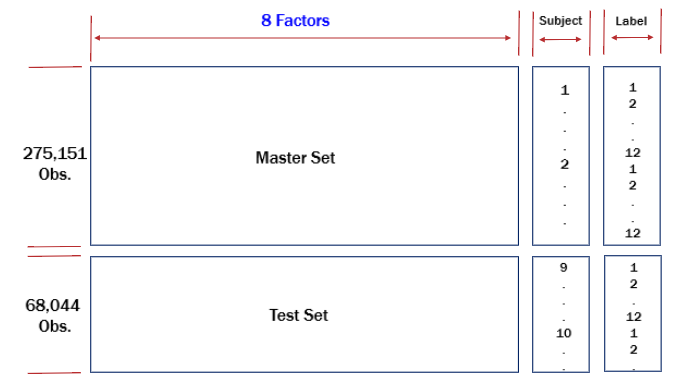
\includegraphics{img/after_dimension_reduction.png}
\caption{title}
\end{figure}

    \section{Classification by Dynamic Time
Warping}\label{classification-by-dynamic-time-warping}

    \section{We assume there is an unknown action from a test
subject}\label{we-assume-there-is-an-unknown-action-from-a-test-subject}

\section{then we compare this unknown action with all actions from a
master subject to get the distance by
DTW}\label{then-we-compare-this-unknown-action-with-all-actions-from-a-master-subject-to-get-the-distance-by-dtw}

\begin{figure}
\centering
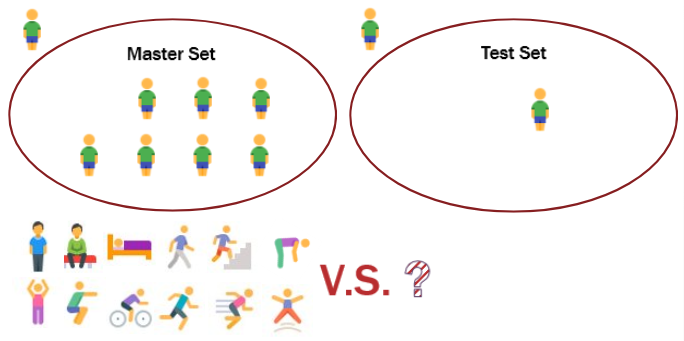
\includegraphics{img/compare_1_subject.png}
\caption{title}
\end{figure}

    \subsubsection{given:}\label{given}

\subsubsection{Method =
classifyOneMovement}\label{method-classifyonemovement}

\subsubsection{Test subject = 9}\label{test-subject-9}

\subsubsection{Test subject action = 3}\label{test-subject-action-3}

\subsubsection{subsample = 5 (for both masterset and
testset)}\label{subsample-5-for-both-masterset-and-testset}

    \subsubsection{Subsample means that every 5 observations we take 1
observation as sample
data}\label{subsample-means-that-every-5-observations-we-take-1-observation-as-sample-data}

    \begin{Verbatim}[commandchars=\\\{\}]
{\color{incolor}In [{\color{incolor}83}]:} \PY{n}{one\PYZus{}move\PYZus{}df} \PY{o}{=} \PY{n}{dtw\PYZus{}experiment}\PY{o}{.}\PY{n}{classifyOneMovement}\PY{p}{(}\PY{n}{mastersubject\PYZus{}index} \PY{o}{=} \PY{l+m+mi}{1}
                                                           \PY{p}{,} \PY{n}{testsubject\PYZus{}index} \PY{o}{=} \PY{l+m+mi}{9}
                                                           \PY{p}{,} \PY{n}{testsubject\PYZus{}action\PYZus{}index} \PY{o}{=} \PY{l+m+mi}{3}
                                                           \PY{p}{,} \PY{n}{subsample} \PY{o}{=} \PY{l+m+mi}{5}\PY{p}{)}
\end{Verbatim}


    \section{As a result, we find that action 3 of subject 1 has the
shortest distance with this unknown
action}\label{as-a-result-we-find-that-action-3-of-subject-1-has-the-shortest-distance-with-this-unknown-action}

    \begin{Verbatim}[commandchars=\\\{\}]
{\color{incolor}In [{\color{incolor}84}]:} \PY{n}{one\PYZus{}move\PYZus{}df}
\end{Verbatim}


\begin{Verbatim}[commandchars=\\\{\}]
{\color{outcolor}Out[{\color{outcolor}84}]:}     MasterSubject  TestSubject  TestSubjectAction  MasterSetAction   Distance  \textbackslash{}
         0               1            9                  3                1 4,230.3188   
         1               1            9                  3                2 3,598.8138   
         2               1            9                  3                3   824.2763   
         3               1            9                  3                4 3,840.3425   
         4               1            9                  3                6 4,099.6455   
         5               1            9                  3                7 3,501.5689   
         6               1            9                  3                8 4,800.5164   
         7               1            9                  3                9 3,705.3588   
         8               1            9                  3               10 4,378.2822   
         9               1            9                  3               11 5,772.7542   
         10              1            9                  3               12 3,399.6842   
         11              1            9                  3                5 4,151.2743   
         
             isMinDistance  isCorrect  
         0          0.0000     0.0000  
         1          0.0000     0.0000  
         2          1.0000     1.0000  
         3          0.0000     0.0000  
         4          0.0000     0.0000  
         5          0.0000     0.0000  
         6          0.0000     0.0000  
         7          0.0000     0.0000  
         8          0.0000     0.0000  
         9          0.0000     0.0000  
         10         0.0000     0.0000  
         11         0.0000     0.0000  
\end{Verbatim}
            
    \section{We compare the unknown action with all other 7 master
subjects}\label{we-compare-the-unknown-action-with-all-other-7-master-subjects}

\begin{figure}
\centering
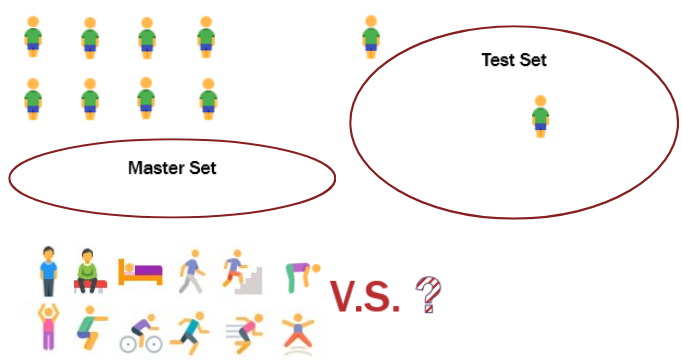
\includegraphics{img/compare_8_subjects.png}
\caption{title}
\end{figure}

    \subsubsection{given:}\label{given}

\subsubsection{Method =
classifyOneMovementByAllMasterSubjects}\label{method-classifyonemovementbyallmastersubjects}

\subsubsection{Test subject = 9}\label{test-subject-9}

\subsubsection{Test subject action = 3}\label{test-subject-action-3}

\subsubsection{subsample = 5 (for both masterset and
testset)}\label{subsample-5-for-both-masterset-and-testset}

    \begin{Verbatim}[commandchars=\\\{\}]
{\color{incolor}In [{\color{incolor}85}]:} \PY{n}{one\PYZus{}move\PYZus{}all\PYZus{}df} \PY{o}{=} \PY{n}{dtw\PYZus{}experiment}\PY{o}{.}\PY{n}{classifyOneMovementByAllMasterSubjects}\PY{p}{(}\PY{n}{testsubject\PYZus{}index} \PY{o}{=} \PY{l+m+mi}{9}
                                                                                   \PY{p}{,} \PY{n}{testsubject\PYZus{}action\PYZus{}index} \PY{o}{=} \PY{l+m+mi}{3}
                                                                                   \PY{p}{,} \PY{n}{subsample} \PY{o}{=} \PY{l+m+mi}{5}\PY{p}{)}
\end{Verbatim}


    \begin{Verbatim}[commandchars=\\\{\}]
{\color{incolor}In [{\color{incolor}86}]:} \PY{n}{one\PYZus{}move\PYZus{}all\PYZus{}df}
\end{Verbatim}


\begin{Verbatim}[commandchars=\\\{\}]
{\color{outcolor}Out[{\color{outcolor}86}]:}     MasterSubject  TestSubject  TestSubjectAction  MasterSetAction   Distance  \textbackslash{}
         0               1            9                  3                1 4,230.3188   
         1               1            9                  3                2 3,598.8138   
         2               1            9                  3                3   824.2763   
         3               1            9                  3                4 3,840.3425   
         4               1            9                  3                6 4,099.6455   
         5               1            9                  3                7 3,501.5689   
         6               1            9                  3                8 4,800.5164   
         7               1            9                  3                9 3,705.3588   
         8               1            9                  3               10 4,378.2822   
         9               1            9                  3               11 5,772.7542   
         10              1            9                  3               12 3,399.6842   
         11              1            9                  3                5 4,151.2743   
         0               2            9                  3                1 3,504.4470   
         1               2            9                  3                2 3,065.8386   
         2               2            9                  3                3 2,182.3837   
         3               2            9                  3                4 3,725.0522   
         4               2            9                  3                6 4,827.6157   
         5               2            9                  3                7 3,838.1323   
         6               2            9                  3                8 5,087.5610   
         7               2            9                  3                9 3,715.4468   
         8               2            9                  3               10 4,380.7275   
         9               2            9                  3               11 4,694.5724   
         10              2            9                  3               12 4,137.0977   
         11              2            9                  3                5 3,915.2197   
         0               3            9                  3                1 4,073.6299   
         1               3            9                  3                2 4,071.8145   
         2               3            9                  3                3   644.4523   
         3               3            9                  3                4 3,958.4766   
         4               3            9                  3                6 4,447.1881   
         5               3            9                  3                7 4,074.8089   
         ..            {\ldots}          {\ldots}                {\ldots}              {\ldots}        {\ldots}   
         6               6            9                  3                8 4,475.8611   
         7               6            9                  3                9 4,230.6220   
         8               6            9                  3               10 4,973.3322   
         9               6            9                  3               11 5,957.2822   
         10              6            9                  3               12 3,429.1949   
         11              6            9                  3                5 4,143.5523   
         0               7            9                  3                1 3,480.9154   
         1               7            9                  3                2 3,162.8123   
         2               7            9                  3                3 2,051.1181   
         3               7            9                  3                4 3,728.5622   
         4               7            9                  3                6 4,158.9974   
         5               7            9                  3                7 2,820.4970   
         6               7            9                  3                8 4,141.4209   
         7               7            9                  3                9 4,104.2171   
         8               7            9                  3               10 4,827.9654   
         9               7            9                  3               11 4,951.6053   
         10              7            9                  3               12 3,128.4612   
         11              7            9                  3                5 3,879.9694   
         0               8            9                  3                1 3,801.6643   
         1               8            9                  3                2 3,062.5393   
         2               8            9                  3                3 1,254.7232   
         3               8            9                  3                4 4,467.2180   
         4               8            9                  3                6 3,850.1746   
         5               8            9                  3                7 2,831.1737   
         6               8            9                  3                8 3,794.1919   
         7               8            9                  3                9 4,203.3343   
         8               8            9                  3               10 4,668.5312   
         9               8            9                  3               11 6,363.4199   
         10              8            9                  3               12 4,201.8544   
         11              8            9                  3                5 3,581.5856   
         
             isMinDistance  isCorrect  
         0          0.0000     0.0000  
         1          0.0000     0.0000  
         2          1.0000     1.0000  
         3          0.0000     0.0000  
         4          0.0000     0.0000  
         5          0.0000     0.0000  
         6          0.0000     0.0000  
         7          0.0000     0.0000  
         8          0.0000     0.0000  
         9          0.0000     0.0000  
         10         0.0000     0.0000  
         11         0.0000     0.0000  
         0          0.0000     0.0000  
         1          0.0000     0.0000  
         2          1.0000     1.0000  
         3          0.0000     0.0000  
         4          0.0000     0.0000  
         5          0.0000     0.0000  
         6          0.0000     0.0000  
         7          0.0000     0.0000  
         8          0.0000     0.0000  
         9          0.0000     0.0000  
         10         0.0000     0.0000  
         11         0.0000     0.0000  
         0          0.0000     0.0000  
         1          0.0000     0.0000  
         2          1.0000     1.0000  
         3          0.0000     0.0000  
         4          0.0000     0.0000  
         5          0.0000     0.0000  
         ..            {\ldots}        {\ldots}  
         6          0.0000     0.0000  
         7          0.0000     0.0000  
         8          0.0000     0.0000  
         9          0.0000     0.0000  
         10         0.0000     0.0000  
         11         0.0000     0.0000  
         0          0.0000     0.0000  
         1          0.0000     0.0000  
         2          1.0000     1.0000  
         3          0.0000     0.0000  
         4          0.0000     0.0000  
         5          0.0000     0.0000  
         6          0.0000     0.0000  
         7          0.0000     0.0000  
         8          0.0000     0.0000  
         9          0.0000     0.0000  
         10         0.0000     0.0000  
         11         0.0000     0.0000  
         0          0.0000     0.0000  
         1          0.0000     0.0000  
         2          1.0000     1.0000  
         3          0.0000     0.0000  
         4          0.0000     0.0000  
         5          0.0000     0.0000  
         6          0.0000     0.0000  
         7          0.0000     0.0000  
         8          0.0000     0.0000  
         9          0.0000     0.0000  
         10         0.0000     0.0000  
         11         0.0000     0.0000  
         
         [96 rows x 7 columns]
\end{Verbatim}
            
    \section{We group the distance by actions and get their mean
distance}\label{we-group-the-distance-by-actions-and-get-their-mean-distance}

\section{We find that action 3 has a shortest mean
distance}\label{we-find-that-action-3-has-a-shortest-mean-distance}

\section{Therefore, we predict that the unknown action is action
3}\label{therefore-we-predict-that-the-unknown-action-is-action-3}

    \begin{Verbatim}[commandchars=\\\{\}]
{\color{incolor}In [{\color{incolor}87}]:} \PY{n}{one\PYZus{}move\PYZus{}all\PYZus{}df}\PY{p}{[}\PY{p}{[}\PY{l+s+s1}{\PYZsq{}}\PY{l+s+s1}{MasterSetAction}\PY{l+s+s1}{\PYZsq{}}\PY{p}{,}\PY{l+s+s1}{\PYZsq{}}\PY{l+s+s1}{Distance}\PY{l+s+s1}{\PYZsq{}}\PY{p}{]}\PY{p}{]}\PY{o}{.}\PY{n}{groupby}\PY{p}{(}\PY{n}{by}\PY{o}{=}\PY{l+s+s2}{\PYZdq{}}\PY{l+s+s2}{MasterSetAction}\PY{l+s+s2}{\PYZdq{}}\PY{p}{)}\PY{o}{.}\PY{n}{mean}\PY{p}{(}\PY{p}{)}
\end{Verbatim}


\begin{Verbatim}[commandchars=\\\{\}]
{\color{outcolor}Out[{\color{outcolor}87}]:}                   Distance
         MasterSetAction           
         1               3,874.5519
         2               3,591.6126
         3               1,203.8124
         4               4,074.1185
         5               4,032.3697
         6               4,480.4650
         7               3,508.7748
         8               4,515.8518
         9               3,937.4887
         10              4,844.4109
         11              5,478.0245
         12              3,730.6905
\end{Verbatim}
            
    \section{We directly get the prediction by method called
"predictOneMovement"}\label{we-directly-get-the-prediction-by-method-called-predictonemovement}

    \begin{Verbatim}[commandchars=\\\{\}]
{\color{incolor}In [{\color{incolor}46}]:} \PY{n}{predictedAction}\PY{p}{,} \PY{n}{predictedResult} \PY{o}{=} \PY{n}{dtw\PYZus{}experiment}\PY{o}{.}\PY{n}{predictOneMovement}\PY{p}{(}\PY{n}{testsubject\PYZus{}index} \PY{o}{=} \PY{l+m+mi}{9}
                                                           \PY{p}{,} \PY{n}{testsubject\PYZus{}action\PYZus{}index} \PY{o}{=} \PY{l+m+mi}{3}
                                                           \PY{p}{,} \PY{n}{subsample} \PY{o}{=} \PY{l+m+mi}{5}\PY{p}{)}
\end{Verbatim}


    \begin{Verbatim}[commandchars=\\\{\}]
{\color{incolor}In [{\color{incolor}47}]:} \PY{n}{predictedAction}
\end{Verbatim}


\begin{Verbatim}[commandchars=\\\{\}]
{\color{outcolor}Out[{\color{outcolor}47}]:} 3
\end{Verbatim}
            
    \begin{Verbatim}[commandchars=\\\{\}]
{\color{incolor}In [{\color{incolor}48}]:} \PY{n}{predictedResult}
\end{Verbatim}


\begin{Verbatim}[commandchars=\\\{\}]
{\color{outcolor}Out[{\color{outcolor}48}]:} True
\end{Verbatim}
            
    \section{For validation, we repeat same steps for remaining actions of
the 2 subjects in Test
Set}\label{for-validation-we-repeat-same-steps-for-remaining-actions-of-the-2-subjects-in-test-set}

\begin{figure}
\centering
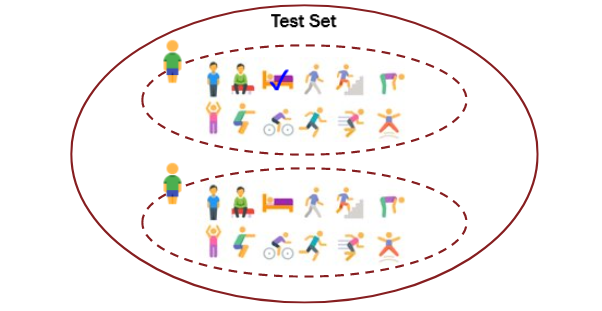
\includegraphics{img/compare_all.png}
\caption{title}
\end{figure}

    \begin{Verbatim}[commandchars=\\\{\}]
{\color{incolor}In [{\color{incolor}49}]:} \PY{n}{predicted\PYZus{}all\PYZus{}df}\PY{p}{,} \PY{n}{accuracy} \PY{o}{=} \PY{n}{dtw\PYZus{}experiment}\PY{o}{.}\PY{n}{PredictAllMovements}\PY{p}{(}\PY{n}{test\PYZus{}subject\PYZus{}index\PYZus{}list} \PY{o}{=} \PY{p}{[}\PY{l+m+mi}{9}\PY{p}{,} \PY{l+m+mi}{10}\PY{p}{]}
                                                            \PY{p}{,} \PY{n}{test\PYZus{}subject\PYZus{}action\PYZus{}index\PYZus{}list} \PY{o}{=} \PY{p}{[}\PY{l+m+mi}{1}\PY{p}{,} \PY{l+m+mi}{2}\PY{p}{,} \PY{l+m+mi}{3}\PY{p}{,} \PY{l+m+mi}{4}\PY{p}{,} \PY{l+m+mi}{5}\PY{p}{,} \PY{l+m+mi}{6}\PY{p}{,} \PY{l+m+mi}{7}\PY{p}{,} \PY{l+m+mi}{8}\PY{p}{,} \PY{l+m+mi}{9}\PY{p}{,} \PY{l+m+mi}{10}\PY{p}{,} \PY{l+m+mi}{11}\PY{p}{,} \PY{l+m+mi}{12}\PY{p}{]}
                                                            \PY{p}{,} \PY{n}{subsample} \PY{o}{=} \PY{l+m+mi}{5}\PY{p}{)}
\end{Verbatim}


    \section{As a result, the overall accuracy score is
0.625}\label{as-a-result-the-overall-accuracy-score-is-0.625}

    \begin{Verbatim}[commandchars=\\\{\}]
{\color{incolor}In [{\color{incolor}50}]:} \PY{n}{accuracy}
\end{Verbatim}


\begin{Verbatim}[commandchars=\\\{\}]
{\color{outcolor}Out[{\color{outcolor}50}]:} 0.625
\end{Verbatim}
            
    \begin{Verbatim}[commandchars=\\\{\}]
{\color{incolor}In [{\color{incolor}51}]:} \PY{n}{predicted\PYZus{}all\PYZus{}df}
\end{Verbatim}


\begin{Verbatim}[commandchars=\\\{\}]
{\color{outcolor}Out[{\color{outcolor}51}]:}     TestSubject  ActualAction  PredictedAction  Result
         0             9             1                1    True
         1             9             2                7   False
         2             9             3                3    True
         3             9             4                4    True
         4             9             5                5    True
         5             9             6                8   False
         6             9             7                9   False
         7             9             8                9   False
         8             9             9                9    True
         9             9            10               10    True
         10            9            11               10   False
         11            9            12               12    True
         12           10             1                1    True
         13           10             2                2    True
         14           10             3                3    True
         15           10             4                4    True
         16           10             5                5    True
         17           10             6                8   False
         18           10             7                9   False
         19           10             8                9   False
         20           10             9                9    True
         21           10            10               10    True
         22           10            11               10   False
         23           10            12               12    True
\end{Verbatim}
            
    \begin{enumerate}
\def\labelenumi{\arabic{enumi})}
\setcounter{enumi}{1}
\tightlist
\item
  Activity set
\end{enumerate}

The activity set is listed in the following:

L1: Standing still (1 min) L2: Sitting and relaxing (1 min) L3: Lying
down (1 min) L4: Walking (1 min) L5: Climbing stairs (1 min) L6: Waist
bends forward (20x) L7: Frontal elevation of arms (20x) L8: Knees
bending (crouching) (20x) L9: Cycling (1 min) L10: Jogging (1 min) L11:
Running (1 min) L12: Jump front \& back (20x)

    \begin{Verbatim}[commandchars=\\\{\}]
{\color{incolor}In [{\color{incolor}52}]:} \PY{k+kn}{import} \PY{n+nn}{matplotlib}\PY{n+nn}{.}\PY{n+nn}{pyplot} \PY{k}{as} \PY{n+nn}{plt}
         \PY{k+kn}{from} \PY{n+nn}{sklearn}\PY{n+nn}{.}\PY{n+nn}{metrics} \PY{k}{import} \PY{n}{confusion\PYZus{}matrix}\PY{p}{,} \PY{n}{accuracy\PYZus{}score}
         \PY{k+kn}{import} \PY{n+nn}{sklearn}\PY{n+nn}{.}\PY{n+nn}{metrics} \PY{k}{as} \PY{n+nn}{metrics}
         
         \PY{n}{columns} \PY{o}{=} \PY{p}{[}\PY{l+s+s1}{\PYZsq{}}\PY{l+s+s1}{Standing}\PY{l+s+s1}{\PYZsq{}}\PY{p}{,} \PY{l+s+s1}{\PYZsq{}}\PY{l+s+s1}{Sitting}\PY{l+s+s1}{\PYZsq{}}\PY{p}{,} \PY{l+s+s1}{\PYZsq{}}\PY{l+s+s1}{Lying}\PY{l+s+s1}{\PYZsq{}}\PY{p}{,} \PY{l+s+s1}{\PYZsq{}}\PY{l+s+s1}{Walking}\PY{l+s+s1}{\PYZsq{}}\PY{p}{,} \PY{l+s+s1}{\PYZsq{}}\PY{l+s+s1}{Climbing}\PY{l+s+s1}{\PYZsq{}}\PY{p}{,} \PY{l+s+s1}{\PYZsq{}}\PY{l+s+s1}{WaistBendsForward}\PY{l+s+s1}{\PYZsq{}}\PY{p}{,} \PY{l+s+s1}{\PYZsq{}}\PY{l+s+s1}{FrontalEvelationArms}\PY{l+s+s1}{\PYZsq{}}
                   \PY{p}{,} \PY{l+s+s1}{\PYZsq{}}\PY{l+s+s1}{Crouching}\PY{l+s+s1}{\PYZsq{}}\PY{p}{,}\PY{l+s+s1}{\PYZsq{}}\PY{l+s+s1}{Cycling}\PY{l+s+s1}{\PYZsq{}}\PY{p}{,}\PY{l+s+s1}{\PYZsq{}}\PY{l+s+s1}{Jogging}\PY{l+s+s1}{\PYZsq{}}\PY{p}{,}\PY{l+s+s1}{\PYZsq{}}\PY{l+s+s1}{Running}\PY{l+s+s1}{\PYZsq{}}\PY{p}{,}\PY{l+s+s1}{\PYZsq{}}\PY{l+s+s1}{Jumping}\PY{l+s+s1}{\PYZsq{}}\PY{p}{]}
         \PY{n}{confusion} \PY{o}{=} \PY{n}{metrics}\PY{o}{.}\PY{n}{confusion\PYZus{}matrix}\PY{p}{(}\PY{n}{predicted\PYZus{}all\PYZus{}df}\PY{p}{[}\PY{l+s+s1}{\PYZsq{}}\PY{l+s+s1}{ActualAction}\PY{l+s+s1}{\PYZsq{}}\PY{p}{]}\PY{p}{,} \PY{n}{predicted\PYZus{}all\PYZus{}df}\PY{p}{[}\PY{l+s+s1}{\PYZsq{}}\PY{l+s+s1}{PredictedAction}\PY{l+s+s1}{\PYZsq{}}\PY{p}{]}\PY{p}{)}
         \PY{n+nb}{print}\PY{p}{(}\PY{n}{metrics}\PY{o}{.}\PY{n}{classification\PYZus{}report}\PY{p}{(}\PY{n}{predicted\PYZus{}all\PYZus{}df}\PY{p}{[}\PY{l+s+s1}{\PYZsq{}}\PY{l+s+s1}{ActualAction}\PY{l+s+s1}{\PYZsq{}}\PY{p}{]}\PY{p}{,} \PY{n}{predicted\PYZus{}all\PYZus{}df}\PY{p}{[}\PY{l+s+s1}{\PYZsq{}}\PY{l+s+s1}{PredictedAction}\PY{l+s+s1}{\PYZsq{}}\PY{p}{]}\PY{p}{,} \PY{n}{target\PYZus{}names}\PY{o}{=}\PY{n}{columns}\PY{p}{)}\PY{p}{)}
         
         \PY{n}{plt}\PY{o}{.}\PY{n}{imshow}\PY{p}{(}\PY{n}{confusion}\PY{p}{,} \PY{n}{cmap}\PY{o}{=}\PY{n}{plt}\PY{o}{.}\PY{n}{cm}\PY{o}{.}\PY{n}{Blues}\PY{p}{,} \PY{n}{interpolation}\PY{o}{=}\PY{l+s+s1}{\PYZsq{}}\PY{l+s+s1}{nearest}\PY{l+s+s1}{\PYZsq{}}\PY{p}{)}
         \PY{n}{plt}\PY{o}{.}\PY{n}{xticks}\PY{p}{(}\PY{p}{[}\PY{l+m+mi}{0}\PY{p}{,} \PY{l+m+mi}{1}\PY{p}{,} \PY{l+m+mi}{2}\PY{p}{,} \PY{l+m+mi}{3}\PY{p}{,} \PY{l+m+mi}{4}\PY{p}{,} \PY{l+m+mi}{5}\PY{p}{,} \PY{l+m+mi}{6}\PY{p}{,} \PY{l+m+mi}{7}\PY{p}{,} \PY{l+m+mi}{8}\PY{p}{,} \PY{l+m+mi}{9}\PY{p}{,} \PY{l+m+mi}{10}\PY{p}{,} \PY{l+m+mi}{11}\PY{p}{]}\PY{p}{,} \PY{n}{columns}\PY{p}{,} \PY{n}{rotation}\PY{o}{=}\PY{l+s+s1}{\PYZsq{}}\PY{l+s+s1}{vertical}\PY{l+s+s1}{\PYZsq{}}\PY{p}{)}
         \PY{n}{plt}\PY{o}{.}\PY{n}{xlabel}\PY{p}{(}\PY{l+s+s1}{\PYZsq{}}\PY{l+s+s1}{Predicted actions}\PY{l+s+s1}{\PYZsq{}}\PY{p}{)}
         \PY{n}{plt}\PY{o}{.}\PY{n}{yticks}\PY{p}{(}\PY{p}{[}\PY{l+m+mi}{0}\PY{p}{,} \PY{l+m+mi}{1}\PY{p}{,} \PY{l+m+mi}{2}\PY{p}{,} \PY{l+m+mi}{3}\PY{p}{,} \PY{l+m+mi}{4}\PY{p}{,} \PY{l+m+mi}{5}\PY{p}{,} \PY{l+m+mi}{6}\PY{p}{,} \PY{l+m+mi}{7}\PY{p}{,} \PY{l+m+mi}{8}\PY{p}{,} \PY{l+m+mi}{9}\PY{p}{,} \PY{l+m+mi}{10}\PY{p}{,} \PY{l+m+mi}{11}\PY{p}{]}\PY{p}{,} \PY{n}{columns}\PY{p}{)}
         \PY{n}{plt}\PY{o}{.}\PY{n}{ylabel}\PY{p}{(}\PY{l+s+s1}{\PYZsq{}}\PY{l+s+s1}{Actual actions}\PY{l+s+s1}{\PYZsq{}}\PY{p}{)}
         \PY{n}{plt}\PY{o}{.}\PY{n}{colorbar}\PY{p}{(}\PY{p}{)}
         
         \PY{n}{plt}\PY{o}{.}\PY{n}{show}\PY{p}{(}\PY{p}{)}
\end{Verbatim}


    \begin{Verbatim}[commandchars=\\\{\}]
C:\textbackslash{}ProgramData\textbackslash{}Anaconda3\textbackslash{}lib\textbackslash{}site-packages\textbackslash{}sklearn\textbackslash{}metrics\textbackslash{}classification.py:1135: UndefinedMetricWarning: Precision and F-score are ill-defined and being set to 0.0 in labels with no predicted samples.
  'precision', 'predicted', average, warn\_for)

    \end{Verbatim}

    \begin{Verbatim}[commandchars=\\\{\}]
                      precision    recall  f1-score   support

            Standing       1.00      1.00      1.00         2
             Sitting       1.00      0.50      0.67         2
               Lying       1.00      1.00      1.00         2
             Walking       1.00      1.00      1.00         2
            Climbing       1.00      1.00      1.00         2
   WaistBendsForward       0.00      0.00      0.00         2
FrontalEvelationArms       0.00      0.00      0.00         2
           Crouching       0.00      0.00      0.00         2
             Cycling       0.33      1.00      0.50         2
             Jogging       0.50      1.00      0.67         2
             Running       0.00      0.00      0.00         2
             Jumping       1.00      1.00      1.00         2

         avg / total       0.57      0.62      0.57        24


    \end{Verbatim}

    \begin{center}
    \adjustimage{max size={0.9\linewidth}{0.9\paperheight}}{output_103_2.png}
    \end{center}
    { \hspace*{\fill} \\}
    
    \section{From the confusion matrix above, we understand
that}\label{from-the-confusion-matrix-above-we-understand-that}

\subsubsection{- DTW can be used for classification
problems​}\label{dtw-can-be-used-for-classification-problems}

\subsubsection{- The actions lie on the diagonal in deep blue, DTW has
good accuracy to classify it. e.g. standing and
jogging}\label{the-actions-lie-on-the-diagonal-in-deep-blue-dtw-has-good-accuracy-to-classify-it.-e.g.-standing-and-jogging}

    \section{Deficiencies}\label{deficiencies}

\subsection{- Small Data Set: Only 10
people​}\label{small-data-set-only-10-people}

\subsection{- It takes time to get DTW
results}\label{it-takes-time-to-get-dtw-results}

    \section{Possible Improvements}\label{possible-improvements}

\subsection{- The accuracy can probably be improved by increasing number
of subjects in master set and the number of observations
used​}\label{the-accuracy-can-probably-be-improved-by-increasing-number-of-subjects-in-master-set-and-the-number-of-observations-used}

\subsection{- Cross validation is expected to be
used​}\label{cross-validation-is-expected-to-be-used}

\subsection{- Rank / weight of features according to
actions}\label{rank-weight-of-features-according-to-actions}

    \section{Code for 3D armadillo case}\label{code-for-3d-armadillo-case}

\subsubsection{source: edX - Microsoft: DAT210x Programming with Python
for Data Science -
Lab4\_1}\label{source-edx---microsoft-dat210x-programming-with-python-for-data-science---lab4_1}

\subsubsection{https://courses.edx.org/courses/course-v1:Microsoft+DAT210x+4T2017/course/}\label{httpscourses.edx.orgcoursescourse-v1microsoftdat210x4t2017course}

    \begin{Verbatim}[commandchars=\\\{\}]
{\color{incolor}In [{\color{incolor}50}]:} \PY{k+kn}{import} \PY{n+nn}{pandas} \PY{k}{as} \PY{n+nn}{pd}
         \PY{k+kn}{import} \PY{n+nn}{matplotlib}\PY{n+nn}{.}\PY{n+nn}{pyplot} \PY{k}{as} \PY{n+nn}{plt}
         \PY{k+kn}{import} \PY{n+nn}{matplotlib}
         
         \PY{k+kn}{from} \PY{n+nn}{mpl\PYZus{}toolkits}\PY{n+nn}{.}\PY{n+nn}{mplot3d} \PY{k}{import} \PY{n}{Axes3D}
         \PY{k+kn}{from} \PY{n+nn}{plyfile} \PY{k}{import} \PY{n}{PlyData}\PY{p}{,} \PY{n}{PlyElement}
         
         \PY{n}{plt}\PY{o}{.}\PY{n}{style}\PY{o}{.}\PY{n}{use}\PY{p}{(}\PY{l+s+s1}{\PYZsq{}}\PY{l+s+s1}{ggplot}\PY{l+s+s1}{\PYZsq{}}\PY{p}{)}
         
         \PY{n}{reduce\PYZus{}factor} \PY{o}{=} \PY{l+m+mi}{100}
         
         \PY{n}{plyfile} \PY{o}{=} \PY{n}{PlyData}\PY{o}{.}\PY{n}{read}\PY{p}{(}\PY{l+s+s1}{\PYZsq{}}\PY{l+s+s1}{PCA/Datasets/stanford\PYZus{}armadillo.ply}\PY{l+s+s1}{\PYZsq{}}\PY{p}{)}
         
         \PY{n}{armadillo} \PY{o}{=} \PY{n}{pd}\PY{o}{.}\PY{n}{DataFrame}\PY{p}{(}\PY{p}{\PYZob{}}
           \PY{l+s+s1}{\PYZsq{}}\PY{l+s+s1}{x}\PY{l+s+s1}{\PYZsq{}}\PY{p}{:}\PY{n}{plyfile}\PY{p}{[}\PY{l+s+s1}{\PYZsq{}}\PY{l+s+s1}{vertex}\PY{l+s+s1}{\PYZsq{}}\PY{p}{]}\PY{p}{[}\PY{l+s+s1}{\PYZsq{}}\PY{l+s+s1}{z}\PY{l+s+s1}{\PYZsq{}}\PY{p}{]}\PY{p}{[}\PY{p}{:}\PY{p}{:}\PY{n}{reduce\PYZus{}factor}\PY{p}{]}\PY{p}{,}
           \PY{l+s+s1}{\PYZsq{}}\PY{l+s+s1}{y}\PY{l+s+s1}{\PYZsq{}}\PY{p}{:}\PY{n}{plyfile}\PY{p}{[}\PY{l+s+s1}{\PYZsq{}}\PY{l+s+s1}{vertex}\PY{l+s+s1}{\PYZsq{}}\PY{p}{]}\PY{p}{[}\PY{l+s+s1}{\PYZsq{}}\PY{l+s+s1}{x}\PY{l+s+s1}{\PYZsq{}}\PY{p}{]}\PY{p}{[}\PY{p}{:}\PY{p}{:}\PY{n}{reduce\PYZus{}factor}\PY{p}{]}\PY{p}{,}
           \PY{l+s+s1}{\PYZsq{}}\PY{l+s+s1}{z}\PY{l+s+s1}{\PYZsq{}}\PY{p}{:}\PY{n}{plyfile}\PY{p}{[}\PY{l+s+s1}{\PYZsq{}}\PY{l+s+s1}{vertex}\PY{l+s+s1}{\PYZsq{}}\PY{p}{]}\PY{p}{[}\PY{l+s+s1}{\PYZsq{}}\PY{l+s+s1}{y}\PY{l+s+s1}{\PYZsq{}}\PY{p}{]}\PY{p}{[}\PY{p}{:}\PY{p}{:}\PY{n}{reduce\PYZus{}factor}\PY{p}{]}
         \PY{p}{\PYZcb{}}\PY{p}{)}
\end{Verbatim}


    \begin{Verbatim}[commandchars=\\\{\}]
{\color{incolor}In [{\color{incolor}51}]:} \PY{k}{def} \PY{n+nf}{do\PYZus{}PCA}\PY{p}{(}\PY{n}{armadillo}\PY{p}{,} \PY{n}{n\PYZus{}components}\PY{p}{,} \PY{n}{svd\PYZus{}solver}\PY{p}{)}\PY{p}{:}
             \PY{c+c1}{\PYZsh{} .. your code here ..}
             \PY{k+kn}{from} \PY{n+nn}{sklearn}\PY{n+nn}{.}\PY{n+nn}{decomposition} \PY{k}{import} \PY{n}{PCA}
             
             \PY{n}{pca} \PY{o}{=} \PY{n}{PCA}\PY{p}{(}\PY{n}{n\PYZus{}components}\PY{o}{=}\PY{n}{n\PYZus{}components}\PY{p}{,} \PY{n}{svd\PYZus{}solver}\PY{o}{=}\PY{n}{svd\PYZus{}solver}\PY{p}{)}
             \PY{n}{pca}\PY{o}{.}\PY{n}{fit}\PY{p}{(}\PY{n}{armadillo}\PY{p}{)}
             \PY{n}{T} \PY{o}{=} \PY{n}{pca}\PY{o}{.}\PY{n}{transform}\PY{p}{(}\PY{n}{armadillo}\PY{p}{)}
             
             \PY{k}{return} \PY{n}{T} 
\end{Verbatim}


    \begin{Verbatim}[commandchars=\\\{\}]
{\color{incolor}In [{\color{incolor}52}]:} \PY{n}{pca} \PY{o}{=} \PY{n}{do\PYZus{}PCA}\PY{p}{(}\PY{n}{armadillo}\PY{p}{,} \PY{l+m+mi}{3}\PY{p}{,} \PY{l+s+s1}{\PYZsq{}}\PY{l+s+s1}{full}\PY{l+s+s1}{\PYZsq{}}\PY{p}{)}
\end{Verbatim}


    \begin{Verbatim}[commandchars=\\\{\}]
{\color{incolor}In [{\color{incolor}53}]:} \PY{n}{fig} \PY{o}{=} \PY{n}{plt}\PY{o}{.}\PY{n}{figure}\PY{p}{(}\PY{p}{)}
         \PY{n}{ax}  \PY{o}{=} \PY{n}{fig}\PY{o}{.}\PY{n}{add\PYZus{}subplot}\PY{p}{(}\PY{l+m+mi}{111}\PY{p}{,} \PY{n}{projection}\PY{o}{=}\PY{l+s+s1}{\PYZsq{}}\PY{l+s+s1}{3d}\PY{l+s+s1}{\PYZsq{}}\PY{p}{)}
         
         \PY{n}{ax}\PY{o}{.}\PY{n}{set\PYZus{}title}\PY{p}{(}\PY{l+s+s1}{\PYZsq{}}\PY{l+s+s1}{Armadillo 3D}\PY{l+s+s1}{\PYZsq{}}\PY{p}{)}
         \PY{n}{ax}\PY{o}{.}\PY{n}{set\PYZus{}xlabel}\PY{p}{(}\PY{l+s+s1}{\PYZsq{}}\PY{l+s+s1}{X}\PY{l+s+s1}{\PYZsq{}}\PY{p}{)}
         \PY{n}{ax}\PY{o}{.}\PY{n}{set\PYZus{}ylabel}\PY{p}{(}\PY{l+s+s1}{\PYZsq{}}\PY{l+s+s1}{Y}\PY{l+s+s1}{\PYZsq{}}\PY{p}{)}
         \PY{n}{ax}\PY{o}{.}\PY{n}{set\PYZus{}zlabel}\PY{p}{(}\PY{l+s+s1}{\PYZsq{}}\PY{l+s+s1}{Z}\PY{l+s+s1}{\PYZsq{}}\PY{p}{)}
         \PY{n}{ax}\PY{o}{.}\PY{n}{scatter}\PY{p}{(}\PY{n}{armadillo}\PY{o}{.}\PY{n}{x}\PY{p}{,} \PY{n}{armadillo}\PY{o}{.}\PY{n}{y}\PY{p}{,} \PY{n}{armadillo}\PY{o}{.}\PY{n}{z}\PY{p}{,} \PY{n}{c}\PY{o}{=}\PY{l+s+s1}{\PYZsq{}}\PY{l+s+s1}{green}\PY{l+s+s1}{\PYZsq{}}\PY{p}{,} \PY{n}{marker}\PY{o}{=}\PY{l+s+s1}{\PYZsq{}}\PY{l+s+s1}{.}\PY{l+s+s1}{\PYZsq{}}\PY{p}{,} \PY{n}{alpha}\PY{o}{=}\PY{l+m+mf}{0.75}\PY{p}{)}
         \PY{n}{plt}\PY{o}{.}\PY{n}{show}\PY{p}{(}\PY{p}{)}
\end{Verbatim}


    \begin{center}
    \adjustimage{max size={0.9\linewidth}{0.9\paperheight}}{output_111_0.png}
    \end{center}
    { \hspace*{\fill} \\}
    
    \section{Get 3 images}\label{get-3-images}

    \begin{Verbatim}[commandchars=\\\{\}]
{\color{incolor}In [{\color{incolor}57}]:} \PY{n}{fig} \PY{o}{=} \PY{n}{plt}\PY{o}{.}\PY{n}{figure}\PY{p}{(}\PY{p}{)}
         \PY{n}{ax} \PY{o}{=} \PY{n}{fig}\PY{o}{.}\PY{n}{add\PYZus{}subplot}\PY{p}{(}\PY{l+m+mi}{111}\PY{p}{)}
         \PY{n}{ax}\PY{o}{.}\PY{n}{set\PYZus{}title}\PY{p}{(}\PY{l+s+s1}{\PYZsq{}}\PY{l+s+s1}{a. his beach pic}\PY{l+s+s1}{\PYZsq{}}\PY{p}{)}
         \PY{n}{ax}\PY{o}{.}\PY{n}{scatter}\PY{p}{(}\PY{n}{pca}\PY{p}{[}\PY{p}{:}\PY{p}{,}\PY{l+m+mi}{0}\PY{p}{]}\PY{p}{,} \PY{n}{pca}\PY{p}{[}\PY{p}{:}\PY{p}{,}\PY{l+m+mi}{2}\PY{p}{]}\PY{p}{,} \PY{n}{c}\PY{o}{=}\PY{l+s+s1}{\PYZsq{}}\PY{l+s+s1}{blue}\PY{l+s+s1}{\PYZsq{}}\PY{p}{,} \PY{n}{marker}\PY{o}{=}\PY{l+s+s1}{\PYZsq{}}\PY{l+s+s1}{.}\PY{l+s+s1}{\PYZsq{}}\PY{p}{,} \PY{n}{alpha}\PY{o}{=}\PY{l+m+mf}{0.75}\PY{p}{)}
         \PY{n}{plt}\PY{o}{.}\PY{n}{show}\PY{p}{(}\PY{p}{)}
\end{Verbatim}


    \begin{center}
    \adjustimage{max size={0.9\linewidth}{0.9\paperheight}}{output_113_0.png}
    \end{center}
    { \hspace*{\fill} \\}
    
    \begin{Verbatim}[commandchars=\\\{\}]
{\color{incolor}In [{\color{incolor}58}]:} \PY{n}{fig} \PY{o}{=} \PY{n}{plt}\PY{o}{.}\PY{n}{figure}\PY{p}{(}\PY{p}{)}
         \PY{n}{ax} \PY{o}{=} \PY{n}{fig}\PY{o}{.}\PY{n}{add\PYZus{}subplot}\PY{p}{(}\PY{l+m+mi}{111}\PY{p}{)}
         \PY{n}{ax}\PY{o}{.}\PY{n}{set\PYZus{}title}\PY{p}{(}\PY{l+s+s1}{\PYZsq{}}\PY{l+s+s1}{b. his car accident pic}\PY{l+s+s1}{\PYZsq{}}\PY{p}{)}
         \PY{n}{ax}\PY{o}{.}\PY{n}{scatter}\PY{p}{(}\PY{n}{pca}\PY{p}{[}\PY{p}{:}\PY{p}{,}\PY{l+m+mi}{0}\PY{p}{]}\PY{p}{,} \PY{n}{pca}\PY{p}{[}\PY{p}{:}\PY{p}{,}\PY{l+m+mi}{1}\PY{p}{]}\PY{p}{,} \PY{n}{c}\PY{o}{=}\PY{l+s+s1}{\PYZsq{}}\PY{l+s+s1}{blue}\PY{l+s+s1}{\PYZsq{}}\PY{p}{,} \PY{n}{marker}\PY{o}{=}\PY{l+s+s1}{\PYZsq{}}\PY{l+s+s1}{.}\PY{l+s+s1}{\PYZsq{}}\PY{p}{,} \PY{n}{alpha}\PY{o}{=}\PY{l+m+mf}{0.75}\PY{p}{)}
         \PY{n}{plt}\PY{o}{.}\PY{n}{show}\PY{p}{(}\PY{p}{)}
\end{Verbatim}


    \begin{center}
    \adjustimage{max size={0.9\linewidth}{0.9\paperheight}}{output_114_0.png}
    \end{center}
    { \hspace*{\fill} \\}
    
    \begin{Verbatim}[commandchars=\\\{\}]
{\color{incolor}In [{\color{incolor}59}]:} \PY{n}{fig} \PY{o}{=} \PY{n}{plt}\PY{o}{.}\PY{n}{figure}\PY{p}{(}\PY{p}{)}
         \PY{n}{ax} \PY{o}{=} \PY{n}{fig}\PY{o}{.}\PY{n}{add\PYZus{}subplot}\PY{p}{(}\PY{l+m+mi}{111}\PY{p}{)}
         \PY{n}{ax}\PY{o}{.}\PY{n}{set\PYZus{}title}\PY{p}{(}\PY{l+s+s1}{\PYZsq{}}\PY{l+s+s1}{c. his embarrassing pic}\PY{l+s+s1}{\PYZsq{}}\PY{p}{)}
         \PY{n}{ax}\PY{o}{.}\PY{n}{scatter}\PY{p}{(}\PY{n}{pca}\PY{p}{[}\PY{p}{:}\PY{p}{,}\PY{l+m+mi}{1}\PY{p}{]}\PY{p}{,} \PY{n}{pca}\PY{p}{[}\PY{p}{:}\PY{p}{,}\PY{l+m+mi}{2}\PY{p}{]}\PY{p}{,} \PY{n}{c}\PY{o}{=}\PY{l+s+s1}{\PYZsq{}}\PY{l+s+s1}{blue}\PY{l+s+s1}{\PYZsq{}}\PY{p}{,} \PY{n}{marker}\PY{o}{=}\PY{l+s+s1}{\PYZsq{}}\PY{l+s+s1}{.}\PY{l+s+s1}{\PYZsq{}}\PY{p}{,} \PY{n}{alpha}\PY{o}{=}\PY{l+m+mf}{0.75}\PY{p}{)}
         \PY{n}{plt}\PY{o}{.}\PY{n}{show}\PY{p}{(}\PY{p}{)}
\end{Verbatim}


    \begin{center}
    \adjustimage{max size={0.9\linewidth}{0.9\paperheight}}{output_115_0.png}
    \end{center}
    { \hspace*{\fill} \\}
    
    \section{get components}\label{get-components}

    \begin{Verbatim}[commandchars=\\\{\}]
{\color{incolor}In [{\color{incolor}60}]:} \PY{n}{fig} \PY{o}{=} \PY{n}{plt}\PY{o}{.}\PY{n}{figure}\PY{p}{(}\PY{p}{)}
         \PY{n}{ax} \PY{o}{=} \PY{n}{fig}\PY{o}{.}\PY{n}{add\PYZus{}subplot}\PY{p}{(}\PY{l+m+mi}{111}\PY{p}{)}
         \PY{n}{ax}\PY{o}{.}\PY{n}{set\PYZus{}title}\PY{p}{(}\PY{l+s+s1}{\PYZsq{}}\PY{l+s+s1}{a. 1st comp and 3rd comp}\PY{l+s+s1}{\PYZsq{}}\PY{p}{)}
         \PY{n}{ax}\PY{o}{.}\PY{n}{scatter}\PY{p}{(}\PY{n}{pca}\PY{p}{[}\PY{p}{:}\PY{p}{,}\PY{l+m+mi}{0}\PY{p}{]}\PY{p}{,} \PY{n}{pca}\PY{p}{[}\PY{p}{:}\PY{p}{,}\PY{l+m+mi}{2}\PY{p}{]}\PY{p}{,} \PY{n}{c}\PY{o}{=}\PY{l+s+s1}{\PYZsq{}}\PY{l+s+s1}{blue}\PY{l+s+s1}{\PYZsq{}}\PY{p}{,} \PY{n}{marker}\PY{o}{=}\PY{l+s+s1}{\PYZsq{}}\PY{l+s+s1}{.}\PY{l+s+s1}{\PYZsq{}}\PY{p}{,} \PY{n}{alpha}\PY{o}{=}\PY{l+m+mf}{0.75}\PY{p}{)}
         \PY{n}{plt}\PY{o}{.}\PY{n}{show}\PY{p}{(}\PY{p}{)}
\end{Verbatim}


    \begin{center}
    \adjustimage{max size={0.9\linewidth}{0.9\paperheight}}{output_117_0.png}
    \end{center}
    { \hspace*{\fill} \\}
    
    \begin{Verbatim}[commandchars=\\\{\}]
{\color{incolor}In [{\color{incolor}61}]:} \PY{n}{fig} \PY{o}{=} \PY{n}{plt}\PY{o}{.}\PY{n}{figure}\PY{p}{(}\PY{p}{)}
         \PY{n}{ax} \PY{o}{=} \PY{n}{fig}\PY{o}{.}\PY{n}{add\PYZus{}subplot}\PY{p}{(}\PY{l+m+mi}{111}\PY{p}{)}
         \PY{n}{ax}\PY{o}{.}\PY{n}{set\PYZus{}title}\PY{p}{(}\PY{l+s+s1}{\PYZsq{}}\PY{l+s+s1}{b. 1st comp and 2nd comp}\PY{l+s+s1}{\PYZsq{}}\PY{p}{)}
         \PY{n}{ax}\PY{o}{.}\PY{n}{scatter}\PY{p}{(}\PY{n}{pca}\PY{p}{[}\PY{p}{:}\PY{p}{,}\PY{l+m+mi}{0}\PY{p}{]}\PY{p}{,} \PY{n}{pca}\PY{p}{[}\PY{p}{:}\PY{p}{,}\PY{l+m+mi}{1}\PY{p}{]}\PY{p}{,} \PY{n}{c}\PY{o}{=}\PY{l+s+s1}{\PYZsq{}}\PY{l+s+s1}{blue}\PY{l+s+s1}{\PYZsq{}}\PY{p}{,} \PY{n}{marker}\PY{o}{=}\PY{l+s+s1}{\PYZsq{}}\PY{l+s+s1}{.}\PY{l+s+s1}{\PYZsq{}}\PY{p}{,} \PY{n}{alpha}\PY{o}{=}\PY{l+m+mf}{0.75}\PY{p}{)}
         \PY{n}{plt}\PY{o}{.}\PY{n}{show}\PY{p}{(}\PY{p}{)}
\end{Verbatim}


    \begin{center}
    \adjustimage{max size={0.9\linewidth}{0.9\paperheight}}{output_118_0.png}
    \end{center}
    { \hspace*{\fill} \\}
    
    \begin{Verbatim}[commandchars=\\\{\}]
{\color{incolor}In [{\color{incolor}62}]:} \PY{n}{fig} \PY{o}{=} \PY{n}{plt}\PY{o}{.}\PY{n}{figure}\PY{p}{(}\PY{p}{)}
         \PY{n}{ax} \PY{o}{=} \PY{n}{fig}\PY{o}{.}\PY{n}{add\PYZus{}subplot}\PY{p}{(}\PY{l+m+mi}{111}\PY{p}{)}
         \PY{n}{ax}\PY{o}{.}\PY{n}{set\PYZus{}title}\PY{p}{(}\PY{l+s+s1}{\PYZsq{}}\PY{l+s+s1}{c. 2nd comp and 3rd comp}\PY{l+s+s1}{\PYZsq{}}\PY{p}{)}
         \PY{n}{ax}\PY{o}{.}\PY{n}{scatter}\PY{p}{(}\PY{n}{pca}\PY{p}{[}\PY{p}{:}\PY{p}{,}\PY{l+m+mi}{1}\PY{p}{]}\PY{p}{,} \PY{n}{pca}\PY{p}{[}\PY{p}{:}\PY{p}{,}\PY{l+m+mi}{2}\PY{p}{]}\PY{p}{,} \PY{n}{c}\PY{o}{=}\PY{l+s+s1}{\PYZsq{}}\PY{l+s+s1}{blue}\PY{l+s+s1}{\PYZsq{}}\PY{p}{,} \PY{n}{marker}\PY{o}{=}\PY{l+s+s1}{\PYZsq{}}\PY{l+s+s1}{.}\PY{l+s+s1}{\PYZsq{}}\PY{p}{,} \PY{n}{alpha}\PY{o}{=}\PY{l+m+mf}{0.75}\PY{p}{)}
         \PY{n}{plt}\PY{o}{.}\PY{n}{show}\PY{p}{(}\PY{p}{)}
\end{Verbatim}


    \begin{center}
    \adjustimage{max size={0.9\linewidth}{0.9\paperheight}}{output_119_0.png}
    \end{center}
    { \hspace*{\fill} \\}
    

    % Add a bibliography block to the postdoc
    
    
    
    \end{document}
